% SayNote Documentation LaTeX Template
% Based on academic thesis structure

\documentclass[12pt,a4paper,final]{report}

% Packages
\usepackage[utf8]{inputenc}
\usepackage[T1]{fontenc}
\usepackage{lmodern}
\usepackage[french,english]{babel}
\usepackage{graphicx}
\usepackage{wrapfig}
\usepackage{caption}
\usepackage{float}
\usepackage{xcolor}
\usepackage{hyperref}
\usepackage{tcolorbox}
\usepackage{listings}
\usepackage{fancyhdr}
\usepackage{tikz}
\usepackage{calc}
\usetikzlibrary{calc}
\usepackage{longtable}
\usepackage{booktabs}
\usepackage{setspace}
\usepackage{geometry}
\usepackage{titlesec}
\usepackage{array}
\usepackage{pifont}
\usepackage{amssymb}
% \usepackage{tocbibind} % For adding LoF, LoT to ToC
\usepackage{tocloft} % For customizing ToC, LoF, LoT

\usepackage{graphicx}

\usepackage{subcaption}

\geometry{a4paper, margin=2.5cm}

% Define SayNote colors
\definecolor{SayNoteBlue}{RGB}{0, 122, 255}
\definecolor{SayNoteGray}{RGB}{142, 142, 147}
\definecolor{SayNoteLightGray}{RGB}{242, 242, 247}
\definecolor{SayNoteDarkGray}{RGB}{44, 44, 46}
\definecolor{coverBorderColor}{RGB}{0, 0, 0}

% Table of contents formatting
\renewcommand{\cftchapfont}{\normalfont}
\renewcommand{\cftchappagefont}{\normalfont}
\renewcommand{\cftsecfont}{\normalfont}
\renewcommand{\cftsecpagefont}{\normalfont}
\renewcommand{\cftsubsecfont}{\normalfont}
\renewcommand{\cftsubsecpagefont}{\normalfont}
\renewcommand{\cftsubsubsecfont}{\normalfont}
\renewcommand{\cftsubsubsecpagefont}{\normalfont}

\renewcommand{\cftchapdotsep}{\cftdotsep} % Add dots for chapters
\renewcommand{\cftchapafterpnum}{\vskip6pt} % Add space after chapter lines

\setlength{\cftbeforechapskip}{0.4em} % Reduce space between chapter entries
\setlength{\cftbeforesecskip}{0.3em} % Reduce space between section entries
\setlength{\cftbeforesubsecskip}{0.2em} % Reduce space between subsection entries

% Set depth of ToC
\setcounter{tocdepth}{3} % Show down to subsubsections
\setcounter{secnumdepth}{3} % Number down to subsubsections

% Format headings to match the style from the example
\titleformat{\chapter}[display]
{\normalfont\Large\bfseries}
{\MakeUppercase{\chaptertitlename} \thechapter}{0.5em}{\MakeUppercase}

\titleformat{\section}
{\normalfont\normalsize\bfseries}
{\thesection}{1em}{}

\titleformat{\subsection}
{\normalfont\normalsize}
{\thesubsection}{1em}{}

\titleformat{\subsubsection}
{\normalfont\normalsize\itshape}
{\thesubsubsection}{1em}{}

% Set headheight to avoid warnings
\setlength{\headheight}{14.5pt}

% Hyperlink settings
\hypersetup{
    colorlinks=true,
    linkcolor=SayNoteBlue,
    citecolor=SayNoteBlue,
    urlcolor=SayNoteBlue,
    pdftitle={SayNote: Voice-Enabled Note-Taking Application},
    pdfauthor={SayNote Team},
    pdfsubject={Technical Documentation},
    pdfkeywords={voice notes, note-taking, mobile app, voice commands}
}

% Custom environments
\newenvironment{featurebox}[1]{
    \begin{tcolorbox}[colback=SayNoteLightGray, colframe=SayNoteBlue, title=#1]
}{
    \end{tcolorbox}
}

\newenvironment{codebox}[1]{
    \begin{tcolorbox}[colback=SayNoteDarkGray, colframe=SayNoteGray, coltext=white, title=#1]
}{
    \end{tcolorbox}
}

% Code listing style
\lstset{
    backgroundcolor=\color{SayNoteDarkGray},
    basicstyle=\footnotesize\ttfamily\color{white},
    breaklines=true,
    captionpos=b,
    commentstyle=\color{SayNoteGray},
    keywordstyle=\color{SayNoteBlue},
    stringstyle=\color{green!50!black},
    numberstyle=\tiny\color{SayNoteGray},
    frame=single,
    rulecolor=\color{SayNoteGray},
    showstringspaces=false,
    tabsize=2
}

% Header and footer
\pagestyle{fancy}
\fancyhf{}
\fancyhead[L]{\slshape\nouppercase{\leftmark}}
\fancyhead[R]{SayNote}
\fancyfoot[C]{\thepage}
\renewcommand{\headrulewidth}{0.4pt}
\renewcommand{\footrulewidth}{0.4pt}

\begin{document}

% Custom title page - matching the reference exactly
\begin{titlepage}
\thispagestyle{empty}

\begin{tikzpicture}[remember picture,overlay]
  % Draw thick black border around the page with reduced top/bottom margins
  \draw [line width=2pt, coverBorderColor] 
    ($(current page.north west) + (0.8cm,-0.4cm)$) 
    rectangle 
    ($(current page.south east) + (-0.8cm,0.4cm)$);
    
  % Draw inner border - thinner line with reduced top/bottom margins
  \draw [line width=0.5pt, coverBorderColor] 
    ($(current page.north west) + (1.1cm,-0.7cm)$) 
    rectangle 
    ($(current page.south east) + (-1.1cm,0.7cm)$);
\end{tikzpicture}

\begin{center}
    \vspace*{0.1cm}
    {\Large \textbf{République Algérienne Démocratique et Populaire}} \\
    \vspace{0.3cm}
    {\large Ministère de l'Enseignement Supérieur et de la Recherche Scientifique} \\
    \vspace{0.3cm}
    {\large Université M'hamed Bougara - Boumerdès} \\
    \vspace{0.6cm}
    
    % University logo
    
\includegraphics[width=4.5cm]{assets/docs/university_logo.png} \\
    \vspace{0.6cm}
    
    {\large Faculté des Sciences} \\
    \vspace{0.2cm}
    {\large Département d'Informatique} \\
    \vspace{0.6cm}
    
    \begin{tabular}{rl}
        \textbf{Domaine} & : Mathématiques Informatique \\
        \textbf{Filière} & : Informatique \\
        \textbf{Spécialité} & : Développement Web et Infographie \\
    \end{tabular} \\
    
    {\small \textit{N° de l'Arrêté d'habilitation de la spécialité : arrêté n°002 du 03/01/2021}} \\
    \vspace{0.7cm}
    
    {\large \textit{\underline{Mémoire de fin d'études en vu de l'obtention du}}} \\
    {\large \textit{\underline{Diplôme de Licence Professionnelle}}} \\
    \vspace{0.7cm}
    
    {\LARGE \textbf{Thème}} \\
    \vspace{0.6cm}
    
    % Create box with project title matching the reference image
    \begin{tikzpicture}
        \node[draw, rounded corners=15pt, line width=1pt, minimum width=14cm, minimum height=3.5cm] {
            \begin{minipage}{13cm}
                \begin{center}
                    \vspace{-0.5cm}
                    \fontsize{22}{26}\selectfont \textbf{SayNote} \\
                    \fontsize{22}{26}\selectfont \textbf{AI-Based Voice Productivity SaaS Application}
                \end{center}
            \end{minipage}
        };
    \end{tikzpicture}
    \vspace{0.8cm}

    \begin{tabular}{p{8cm}p{6cm}}
        \textbf{Présenté par :} & \textbf{Supervisé par :} \\
        BENHADJER Foudhil Abdellah & CHAOUCHE Ali \\
        SADAOUI Ayoub & \\
        HAFSAOUI Abderahim & \\
    \end{tabular} \\
    \vspace{0.8cm}
    
    {\normalsize Soutenu le \underline{24/06/2024} Devant le jury composé de} \\
    \vspace{0.4cm}
    \begin{tabular}{lll}
        HAMICHE Mokhtar & : & Examinateur \\
        BELKASMI Djamel & : & Examinateur \\
        YAHIATENE Youcef & : & Président \\
    \end{tabular}
\end{center}
\end{titlepage}

\newpage
% Create a special page for TABLE DES MATIERES
\thispagestyle{empty}
\begin{center}
    \vspace*{1cm}
    \Huge{\textbf{TABLE DES MATIÈRES}}
    \vspace{1.5cm}
\end{center}
\renewcommand{\contentsname}{}
\tableofcontents
\thispagestyle{empty}
\newpage

% List of figures
\thispagestyle{empty}
\begin{center}
    \vspace*{1cm}
    \Huge{\textbf{TABLE DES FIGURES}}
    \vspace{1.5cm}
\end{center}
\renewcommand{\listfigurename}{}
\listoffigures
\addcontentsline{toc}{chapter}{TABLE DES FIGURES}
\thispagestyle{empty}
\newpage

% List of tables
\thispagestyle{empty}
\begin{center}
    \vspace*{1cm}
    \Huge{\textbf{TABLE DES TABLEAUX}}
    \vspace{1.5cm}
\end{center}
\renewcommand{\listtablename}{}
\listoftables
\addcontentsline{toc}{chapter}{TABLE DES TABLEAUX}
\thispagestyle{empty}
\newpage

% Introduction chapter
\chapter*{INTRODUCTION}
\addcontentsline{toc}{chapter}{INTRODUCTION}
% Introduction Chapter for SayNote Documentation

% --- Introduction non numérotée ---
\begin{center}
\textbf{\large Introduction du Chapitre}
\end{center}

\noindent
Ce chapitre présente le contexte, les objectifs et la portée du projet SayNote. Il offre une vue d'ensemble sur la motivation derrière l'application, les principales fonctionnalités attendues, ainsi que la structure du document. Le lecteur acquerra une compréhension globale du projet avant d'entrer dans les détails techniques et conceptuels des chapitres suivants.

\thispagestyle{fancy}

\vspace{1cm}

Dans un monde en constante évolution, la technologie est devenue essentielle pour transformer divers secteurs, y compris le domaine de la prise de notes et de la création de documents. Avec l'essor des assistants vocaux et des technologies de reconnaissance vocale, le potentiel d'innovation dans la façon dont nous capturons et organisons nos pensées est immense.

SayNote représente une approche innovante pour capturer, organiser et affiner les pensées principalement par commandes vocales, complétée par un éditeur intuitif basé sur des blocs. L'application vise à être la solution de référence pour les utilisateurs qui valorisent la rapidité, l'efficacité et la flexibilité de la saisie vocale, sans sacrifier les riches capacités d'édition des éditeurs de blocs modernes.

\vspace{0.5cm}

L'idée principale derrière SayNote est de créer une expérience fluide de prise de notes et de création de documents, optimisée pour les appareils mobiles. L'application s'adresse aux étudiants, aux professionnels, aux écrivains et à toute personne ayant besoin de noter rapidement des idées, d'organiser des notes ou de rédiger des documents en déplacement.

\vspace{0.5cm}

La vision de SayNote est de devenir l'application de choix pour ceux qui cherchent à maximiser leur productivité en transformant la parole en contenu structuré et organisé. En combinant la puissance des commandes vocales avec l'organisation intuitive des éditeurs de blocs, SayNote offre une solution innovante aux défis de la prise de notes traditionnelle.

\vspace{1cm}

\section*{Objectifs du projet}
\addcontentsline{toc}{section}{Objectifs du projet}

Les objectifs principaux du projet SayNote sont :

\begin{itemize}
    \item Développer une application mobile entièrement fonctionnelle permettant aux utilisateurs de créer et d'éditer des notes via des commandes vocales.
    \item Implémenter un éditeur basé sur BlockNote.js offrant une expérience d'édition par blocs similaire à Notion.
    \item Assurer une transcription vocale de haute fidélité et une analyse intelligente des intentions de l'utilisateur.
    \item Créer une interface utilisateur intuitive et conviviale optimisée pour les appareils mobiles.
    \item Fournir une application web complémentaire pour une expérience cross-platform complète.
\end{itemize}

\vspace{1cm}

\section*{Portée du document}
\addcontentsline{toc}{section}{Portée du document}

Ce document sert de guide complet pour l'application SayNote, couvrant sa base conceptuelle, son architecture technique, les détails d'implémentation, la conception de l'expérience utilisateur et l'identité visuelle. Il est destiné aux développeurs, designers et parties prenantes impliqués dans le projet, fournissant une compréhension approfondie de la structure et de la fonctionnalité de l'application.

La documentation est organisée en plusieurs chapitres, chacun couvrant un aspect spécifique du développement et de la conception de SayNote :

\begin{itemize}
    \item \textbf{Étude préalable} : Analyse du problème, objectifs du projet et solutions proposées.
    \item \textbf{Planification et conception UX} : Méthodologie de développement, recherche utilisateur et conception du système.
    \item \textbf{Implémentation et développement} : Architecture technique, technologies utilisées et détails d'implémentation.
    \item \textbf{Identité visuelle} : Conception de la marque, éléments visuels et interfaces utilisateur.
\end{itemize}

Ce document servira de référence tout au long du cycle de développement du projet et pourra être utilisé comme base pour la formation, la maintenance et l'évolution future de l'application SayNote. 

% --- Conclusion non numérotée ---
\vspace{1cm}
\begin{center}
\textbf{\large Conclusion du Chapitre}
\end{center}

\noindent
En résumé, ce chapitre introductif a permis de cerner le contexte, les objectifs et la portée du projet SayNote. Il prépare le lecteur à explorer les aspects détaillés de la solution, depuis l'étude préalable jusqu'à la conception, l'implémentation et l'identité visuelle, en fournissant une base solide pour la compréhension du reste de la documentation.

% Chapter 1: Etude préalable
\chapter{ETUDE PREALABLE}
% SayNote - Chapitre 2 : Étude de l’existant
% Ce chapitre analyse l’état actuel de la prise de notes et de la gestion d’informations, en s’appuyant sur les pratiques, outils et défis rencontrés par les utilisateurs.

% --- Introduction non numérotée ---
\begin{center}
\textbf{\large Introduction du Chapitre}
\end{center}

\noindent
Ce chapitre dresse un état des lieux des pratiques actuelles de prise de notes et de gestion d’informations, en identifiant les méthodes utilisées, les difficultés rencontrées et les limites des solutions existantes. L’objectif est de comprendre le contexte et les besoins réels des utilisateurs avant toute proposition de solution.

\section{Introduction}

La prise de notes et la gestion d’informations sont des activités essentielles pour de nombreux profils : étudiants, professionnels, créatifs, etc. Malgré la diversité des outils disponibles, de nombreux utilisateurs rencontrent encore des obstacles dans l’organisation, la fiabilité et l’accessibilité de leurs notes. Ce chapitre propose une analyse détaillée de l’existant afin de mettre en lumière les défis à relever.

\section{Contexte de la prise de notes}

La prise de notes intervient dans des contextes variés : réunions, cours, brainstorming, déplacements, etc. Les utilisateurs cherchent à capturer rapidement des idées, à structurer des informations, et à pouvoir y accéder facilement sur différents supports (papier, ordinateur, mobile). L’évolution des usages montre une transition progressive du papier vers les outils numériques, sans pour autant résoudre tous les problèmes liés à la gestion efficace des notes.

\section{Méthodes actuelles de gestion des notes et informations}

La gestion des notes repose aujourd’hui sur une grande diversité de méthodes et d’outils, qu’on peut regrouper en plusieurs catégories :

\subsection{Prise de notes manuelle}
\begin{itemize}
    \item Utilisation de carnets, feuilles volantes, post-its.
    \item Facilité d’accès mais risque élevé de perte, de désorganisation ou d’oubli.
    \item Difficulté à rechercher ou à partager l’information.
\end{itemize}

\subsection{Outils numériques classiques}
\begin{itemize}
    \item Logiciels de traitement de texte (Word, Google Docs), tableurs, emails.
    \item Avantages : sauvegarde, partage, édition facile.
    \item Limites : structure peu adaptée à la prise de notes rapide, fragmentation des fichiers, manque de synchronisation multi-appareils.
\end{itemize}

\subsection{Applications spécialisées de prise de notes}
\begin{itemize}
    \item Applications comme Notion, Evernote, OneNote, Google Keep, Apple Notes.
    \item Fonctions avancées : organisation hiérarchique, recherche, étiquettes, synchronisation cloud, prise de notes vocale.
    \item Limitations relevées par les utilisateurs :
    \begin{itemize}
        \item Transcription vocale parfois imprécise, surtout en environnement bruyant ou multilingue.
        \item Fonctionnalités inégales entre versions web et mobile.
        \item Interface parfois complexe ou non adaptée à l’usage mobile rapide.
        \item Problèmes de synchronisation ou de perte de données occasionnelle.
        \item Dépendance à la connexion internet pour certaines fonctions.
        \item Gestion des historiques ou des versions parfois limitée.
    \end{itemize}
\end{itemize}

\subsection{Organisation et archivage}
\begin{itemize}
    \item Utilisation de dossiers, tags, favoris, et moteurs de recherche pour classer et retrouver l’information.
    \item Archivage manuel ou automatisé, mais risque de fragmentation et de perte de contexte.
    \item Difficulté à maintenir une organisation cohérente sur le long terme.
\end{itemize}

\section{Défis et limitations de l’existant}

Malgré la richesse des outils disponibles, plusieurs défis majeurs persistent :
\begin{itemize}
    \item \textbf{Efficacité limitée :} La prise de notes rapide et structurée reste difficile, en particulier lors de situations de mobilité ou de multitâche.
    \item \textbf{Précision et fiabilité :} Les erreurs de transcription, la perte de données ou les problèmes de synchronisation peuvent nuire à la confiance dans l’outil.
    \item \textbf{Fragmentation de l’information :} La multiplication des supports et applications conduit à une dispersion des notes, rendant leur gestion et leur recherche complexes.
    \item \textbf{Accessibilité et ergonomie :} Les interfaces ne sont pas toujours adaptées à tous les usages (mobile, desktop, voix), ce qui limite l’adoption ou l’efficacité.
    \item \textbf{Confidentialité et dépendance :} La dépendance à des services cloud externes soulève des questions de confidentialité et de pérennité des données.
\end{itemize}

\section{Problématique}

Face à ces limites, de nombreux utilisateurs expriment le besoin d’une solution qui soit à la fois rapide, fiable, accessible sur tous leurs appareils, et capable d’organiser l’information sans effort supplémentaire. La question centrale devient alors : comment concevoir un outil de prise de notes qui réponde réellement aux attentes de mobilité, de fiabilité, d’ergonomie et de sécurité des utilisateurs modernes ?

\section{Conclusion}

Ce chapitre a permis de dresser un panorama complet des pratiques et outils actuels de prise de notes, en mettant en évidence leurs forces et faiblesses. Cette analyse de l’existant constitue le socle sur lequel s’appuiera la réflexion autour d’une solution innovante, présentée dans le chapitre suivant.

% --- Conclusion non numérotée ---
\vspace{1cm}
\begin{center}
\textbf{\large Conclusion du Chapitre}
\end{center}

\noindent
En conclusion, l’étude de l’existant révèle des besoins réels et non totalement satisfaits en matière de prise de notes et de gestion d’informations. Les prochaines sections proposeront une réponse adaptée à ces enjeux, en s’appuyant sur les constats établis ici.
\section{Problématiques}

La prise de notes traditionnelle, qu'elle soit manuscrite ou numérique, présente plusieurs défis majeurs que nous avons identifiés à travers notre recherche et nos observations:

\subsection{Limites de la saisie manuelle}

La saisie manuelle de notes, que ce soit à l'aide d'un stylo et papier ou d'un clavier, présente plusieurs inconvénients:

\begin{itemize}
    \item \textbf{Vitesse limitée:} La vitesse de frappe moyenne (40-60 mots par minute) ou d'écriture manuscrite (10-30 mots par minute) est souvent insuffisante pour capturer efficacement des informations lors de réunions, conférences ou sessions de brainstorming rapides.
    
    \item \textbf{Fatigue et inconfort:} La saisie prolongée peut entraîner une fatigue des mains et des poignets, particulièrement sur les appareils mobiles où les claviers virtuels offrent une expérience sous-optimale.
    
    \item \textbf{Attention divisée:} Le fait de devoir se concentrer sur la saisie divise l'attention de l'utilisateur, réduisant sa capacité à écouter activement ou à participer pleinement à une discussion.
\end{itemize}

\subsection{Accessibilité réduite}

Les méthodes traditionnelles de prise de notes présentent des obstacles d'accessibilité significatifs:

\begin{itemize}
    \item \textbf{Mobilité réduite:} Les personnes souffrant de limitations motrices peuvent éprouver des difficultés considérables avec la saisie manuelle.
    
    \item \textbf{Situations multi-tâches:} De nombreux contextes (conduite, marche, exercice) rendent la saisie manuelle difficile voire impossible.
    
    \item \textbf{Barrières linguistiques:} Pour les utilisateurs non natifs d'une langue, la saisie écrite peut présenter des difficultés supplémentaires par rapport à l'expression orale.
\end{itemize}

\subsection{Complexité de structuration}

L'organisation et la structuration efficaces des notes représentent un défi majeur:

\begin{itemize}
    \item \textbf{Effort post-capture:} La transformation de notes brutes en contenu structuré et organisé nécessite souvent un effort supplémentaire considérable.
    
    \item \textbf{Rigidité des formats:} De nombreuses applications de prise de notes offrent des structures rigides qui limitent la flexibilité et l'adaptabilité aux différents types de contenu.
    
    \item \textbf{Courbe d'apprentissage:} Les éditeurs avancés comme Notion requièrent un investissement initial en temps pour maîtriser leurs fonctionnalités.
\end{itemize}































\section{Conclusion}


% --- Conclusion non numérotée ---
\vspace{1cm}
\begin{center}
\textbf{\large Conclusion du Chapitre}
\end{center}

\noindent
En conclusion, cette étude préalable a permis de cerner les besoins, les défis et les opportunités du secteur de la prise de notes. Cette étude préalable met en évidence les besoins, les défis et les opportunités du secteur de la prise de notes. Elle conclut sur l'importance d'une réflexion approfondie pour répondre aux attentes des utilisateurs, sans anticiper sur la solution à proposer.

% Chapter 2: Planification et Conception UX
\chapter{PLANIFICATION ET CONCEPTION UX}
% SayNote - Chapitre II: Planification et Conception UX
% Ce chapitre présente la planification du projet et la conception de l'expérience utilisateur


    
    \subsection{Planification du projet}
    
    \subsubsection{Méthodologie de planification}
    
    Pour le développement de SayNote, nous avons adopté une approche agile, plus précisément la méthodologie Scrum, complétée par des éléments de Design Thinking pour la conception UX. Cette combinaison nous permet d'itérer rapidement tout en gardant l'utilisateur au centre de notre processus de conception.
    
    \paragraph{Approche Agile Scrum}
    
    L'approche Scrum a été choisie pour sa flexibilité et sa capacité à s'adapter aux changements inhérents au développement d'un produit innovant comme SayNote. Nous avons organisé notre travail en sprints de deux semaines, chacun comportant les événements standards de Scrum:
    
    \begin{itemize}
        \item \textbf{Sprint Planning:} Au début de chaque sprint, l'équipe sélectionne les tâches du Product Backlog à réaliser, en se basant sur leur priorité et la capacité de l'équipe.
        
        \item \textbf{Daily Stand-up:} Réunions quotidiennes de 15 minutes pour synchroniser les activités et identifier les obstacles.
        
        \item \textbf{Sprint Review:} À la fin de chaque sprint, l'équipe présente les fonctionnalités développées aux parties prenantes pour obtenir des retours.
        
        \item \textbf{Sprint Retrospective:} L'équipe analyse ce qui a bien fonctionné et ce qui peut être amélioré pour le prochain sprint.
    \end{itemize}
    
    Cette approche nous permet de livrer régulièrement des incréments de produit fonctionnels et d'ajuster notre direction en fonction des retours utilisateurs et des défis techniques rencontrés.
    
    \paragraph{Design Thinking pour l'UX}
    
    En parallèle de Scrum, nous avons intégré le processus de Design Thinking pour la conception de l'expérience utilisateur, qui comprend cinq phases:
    
    \begin{enumerate}
        \item \textbf{Empathie:} Comprendre profondément les besoins, les frustrations et les aspirations des utilisateurs potentiels à travers des entretiens et des observations.
        
        \item \textbf{Définition:} Synthétiser les connaissances acquises pour définir clairement les problèmes à résoudre.
        
        \item \textbf{Idéation:} Générer un large éventail d'idées et de solutions potentielles sans contraintes initiales.
        
        \item \textbf{Prototypage:} Créer des représentations tangibles des solutions les plus prometteuses.
        
        \item \textbf{Test:} Recueillir les retours des utilisateurs sur les prototypes pour affiner et améliorer les solutions.
    \end{enumerate}
    
    Cette approche centrée sur l'utilisateur est particulièrement pertinente pour SayNote, où l'interaction vocale nécessite une compréhension fine des attentes et des comportements des utilisateurs.
    
        
    \subsubsection{Planification}
    
    \paragraph{Roadmap du projet}
    
    La roadmap de SayNote a été structurée en quatre phases principales, chacune comportant plusieurs sprints:
    
    \begin{enumerate}
        \item \textbf{Phase de recherche et de conception (2 mois):}
        \begin{itemize}
            \item Recherche utilisateur et analyse concurrentielle
            \item Définition des personas et des scénarios d'utilisation
            \item Conception de l'architecture du système
            \item Wireframing et prototypage initial
        \end{itemize}
        
        \item \textbf{Phase de développement MVP (4 mois):}
        \begin{itemize}
            \item Mise en place de l'infrastructure technique
            \item Développement du backend et de l'API
            \item Implémentation de l'éditeur de notes par blocs (avec BlockNote.js)
            \item Intégration de la reconnaissance vocale de base
            \item Développement de l'interface utilisateur mobile (Expo/React Native)
        \end{itemize}
        
        \item \textbf{Phase d'amélioration et d'expansion (3 mois):}
        \begin{itemize}
            \item Optimisation des algorithmes de traitement du langage naturel
            \item Expansion des commandes vocales supportées
            \item Développement de l'interface web
            \item Implémentation des fonctionnalités de sous-pages et de hiérarchie de notes
        \end{itemize}
        
        \item \textbf{Phase de finalisation et de lancement (1 mois):}
        \begin{itemize}
            \item Tests utilisateurs approfondis
            \item Correction des bugs et optimisations finales
            \item Préparation du matériel marketing
            \item Lancement officiel de l'application
        \end{itemize}
    \end{enumerate}
    
    % Explication brève avant chaque figure
        \begin{figure}[htbp]
        \centering
        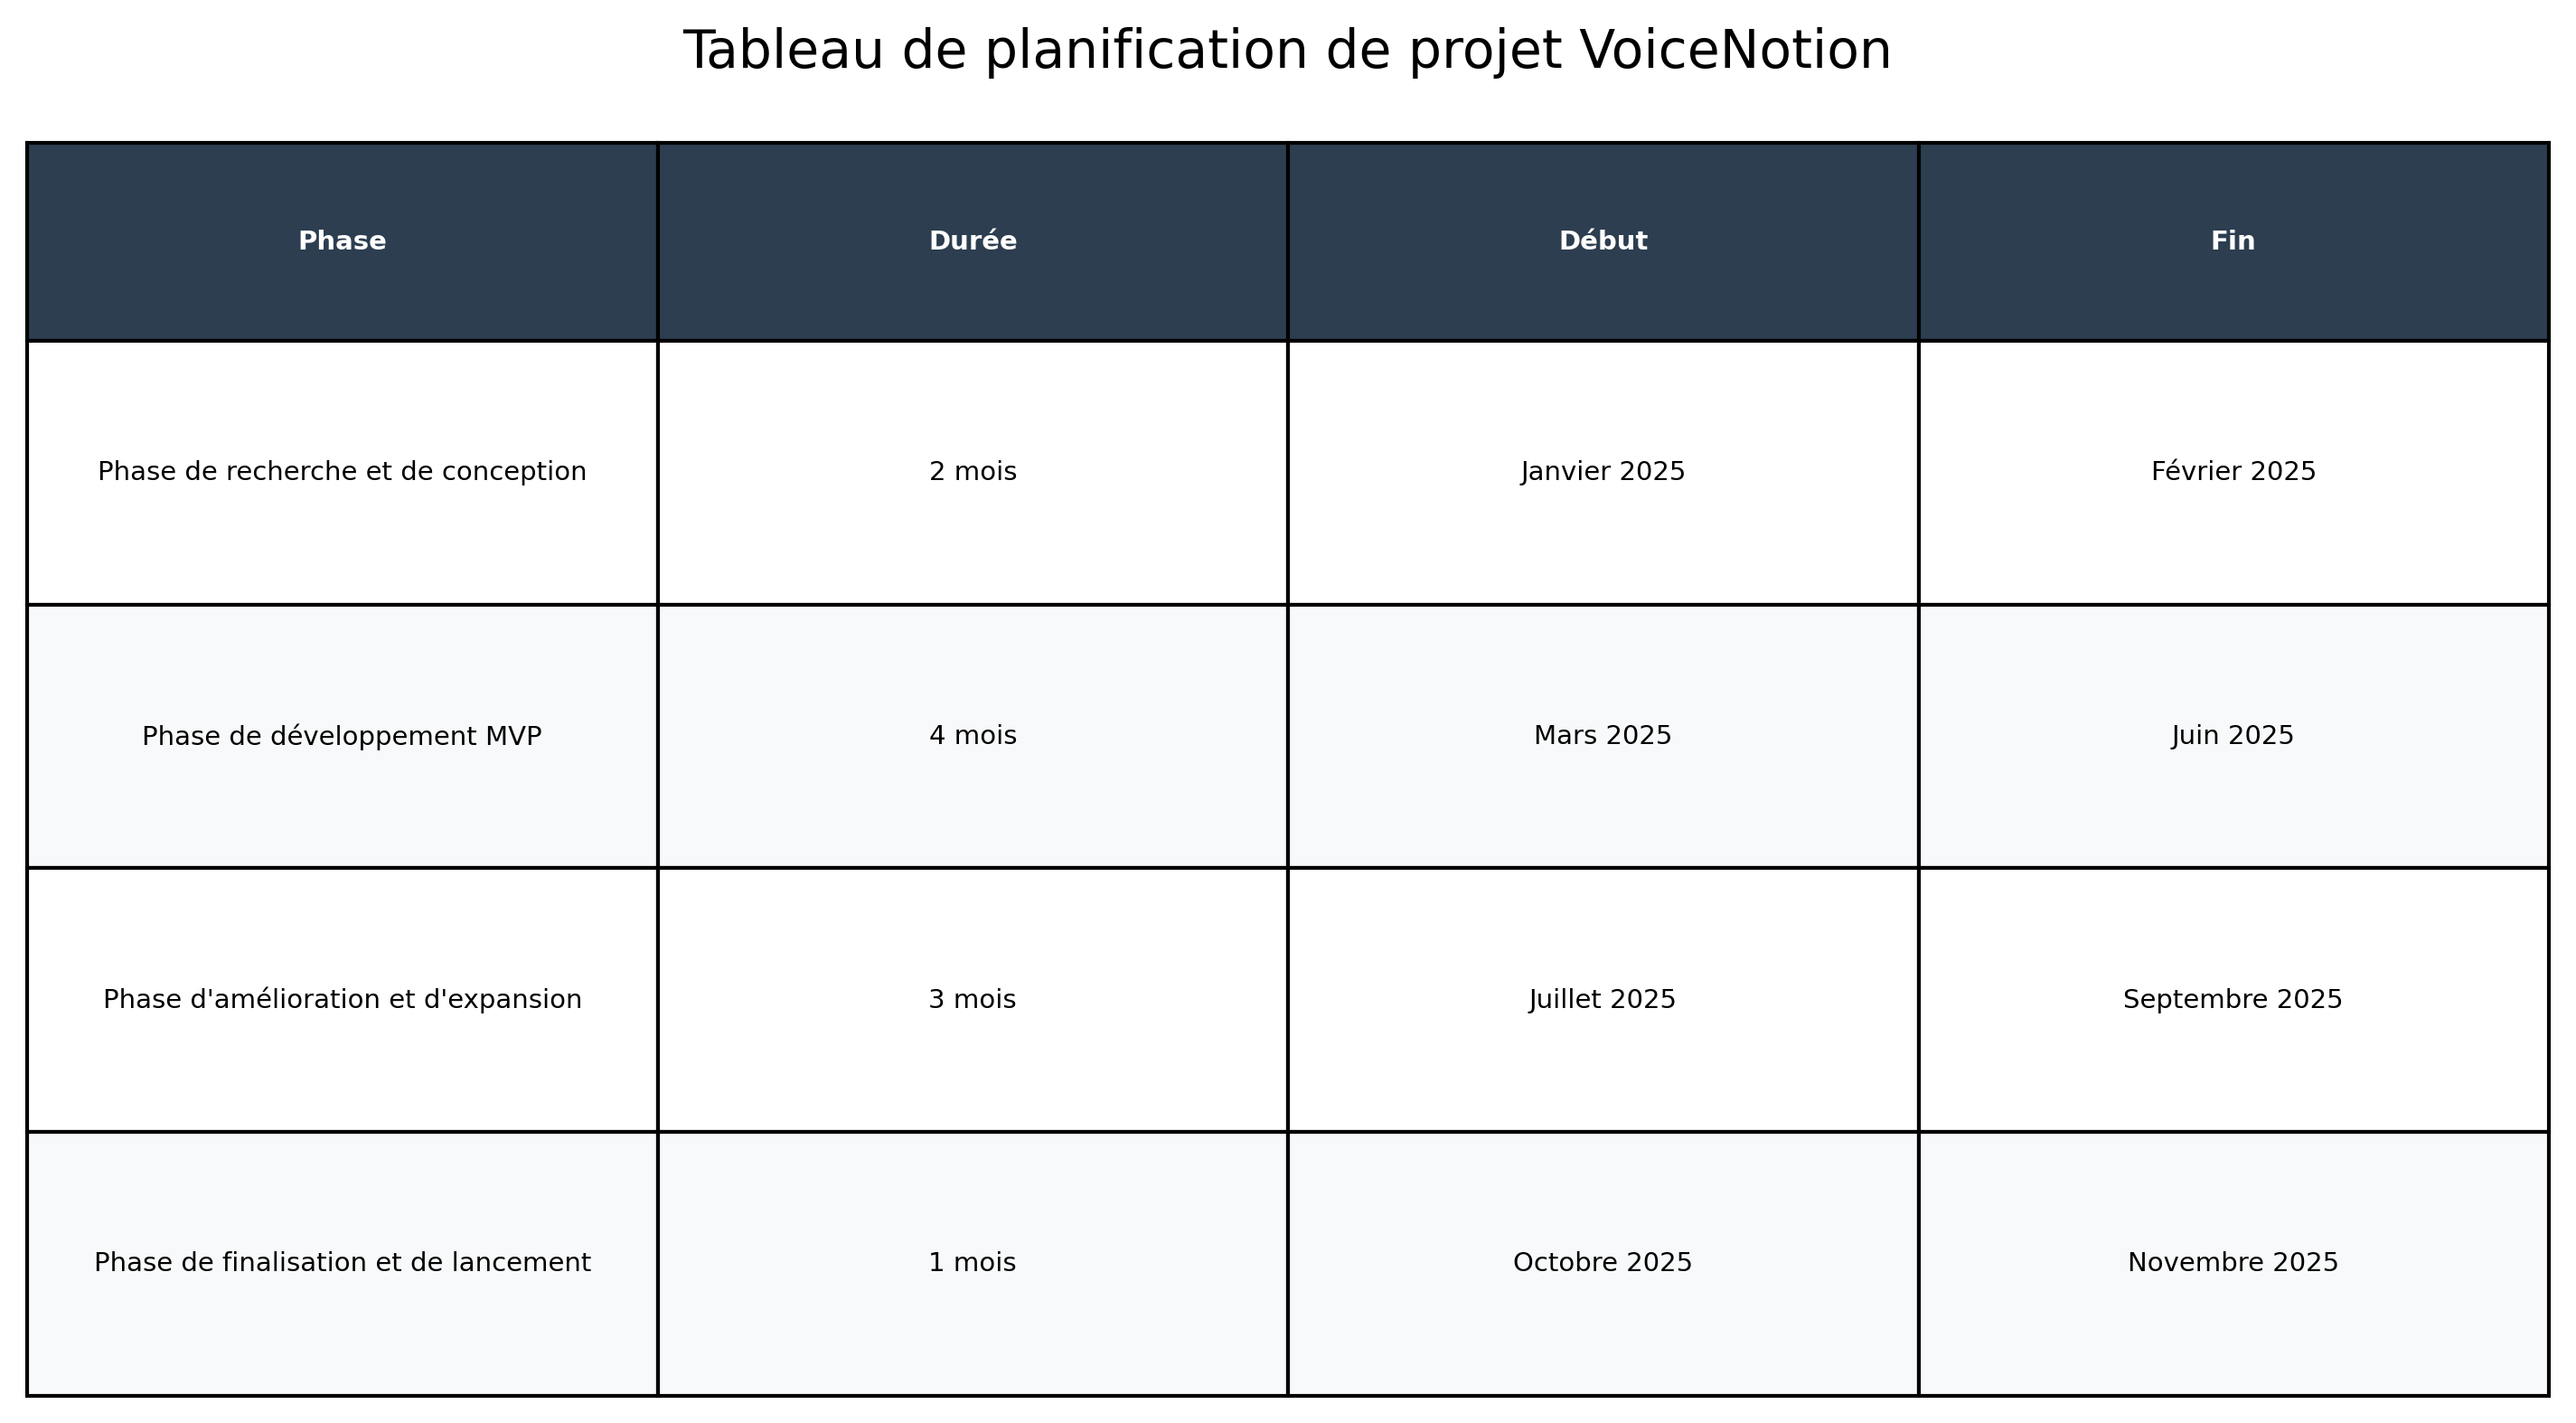
\includegraphics[width=0.9\textwidth]{assets/docs/planification_table.png}
        \caption{Tableau de planification de projet}
        \label{fig:planification_table}
    \end{figure}
    
    % Explication brève avant chaque figure
        \begin{figure}[htbp]
        \centering
        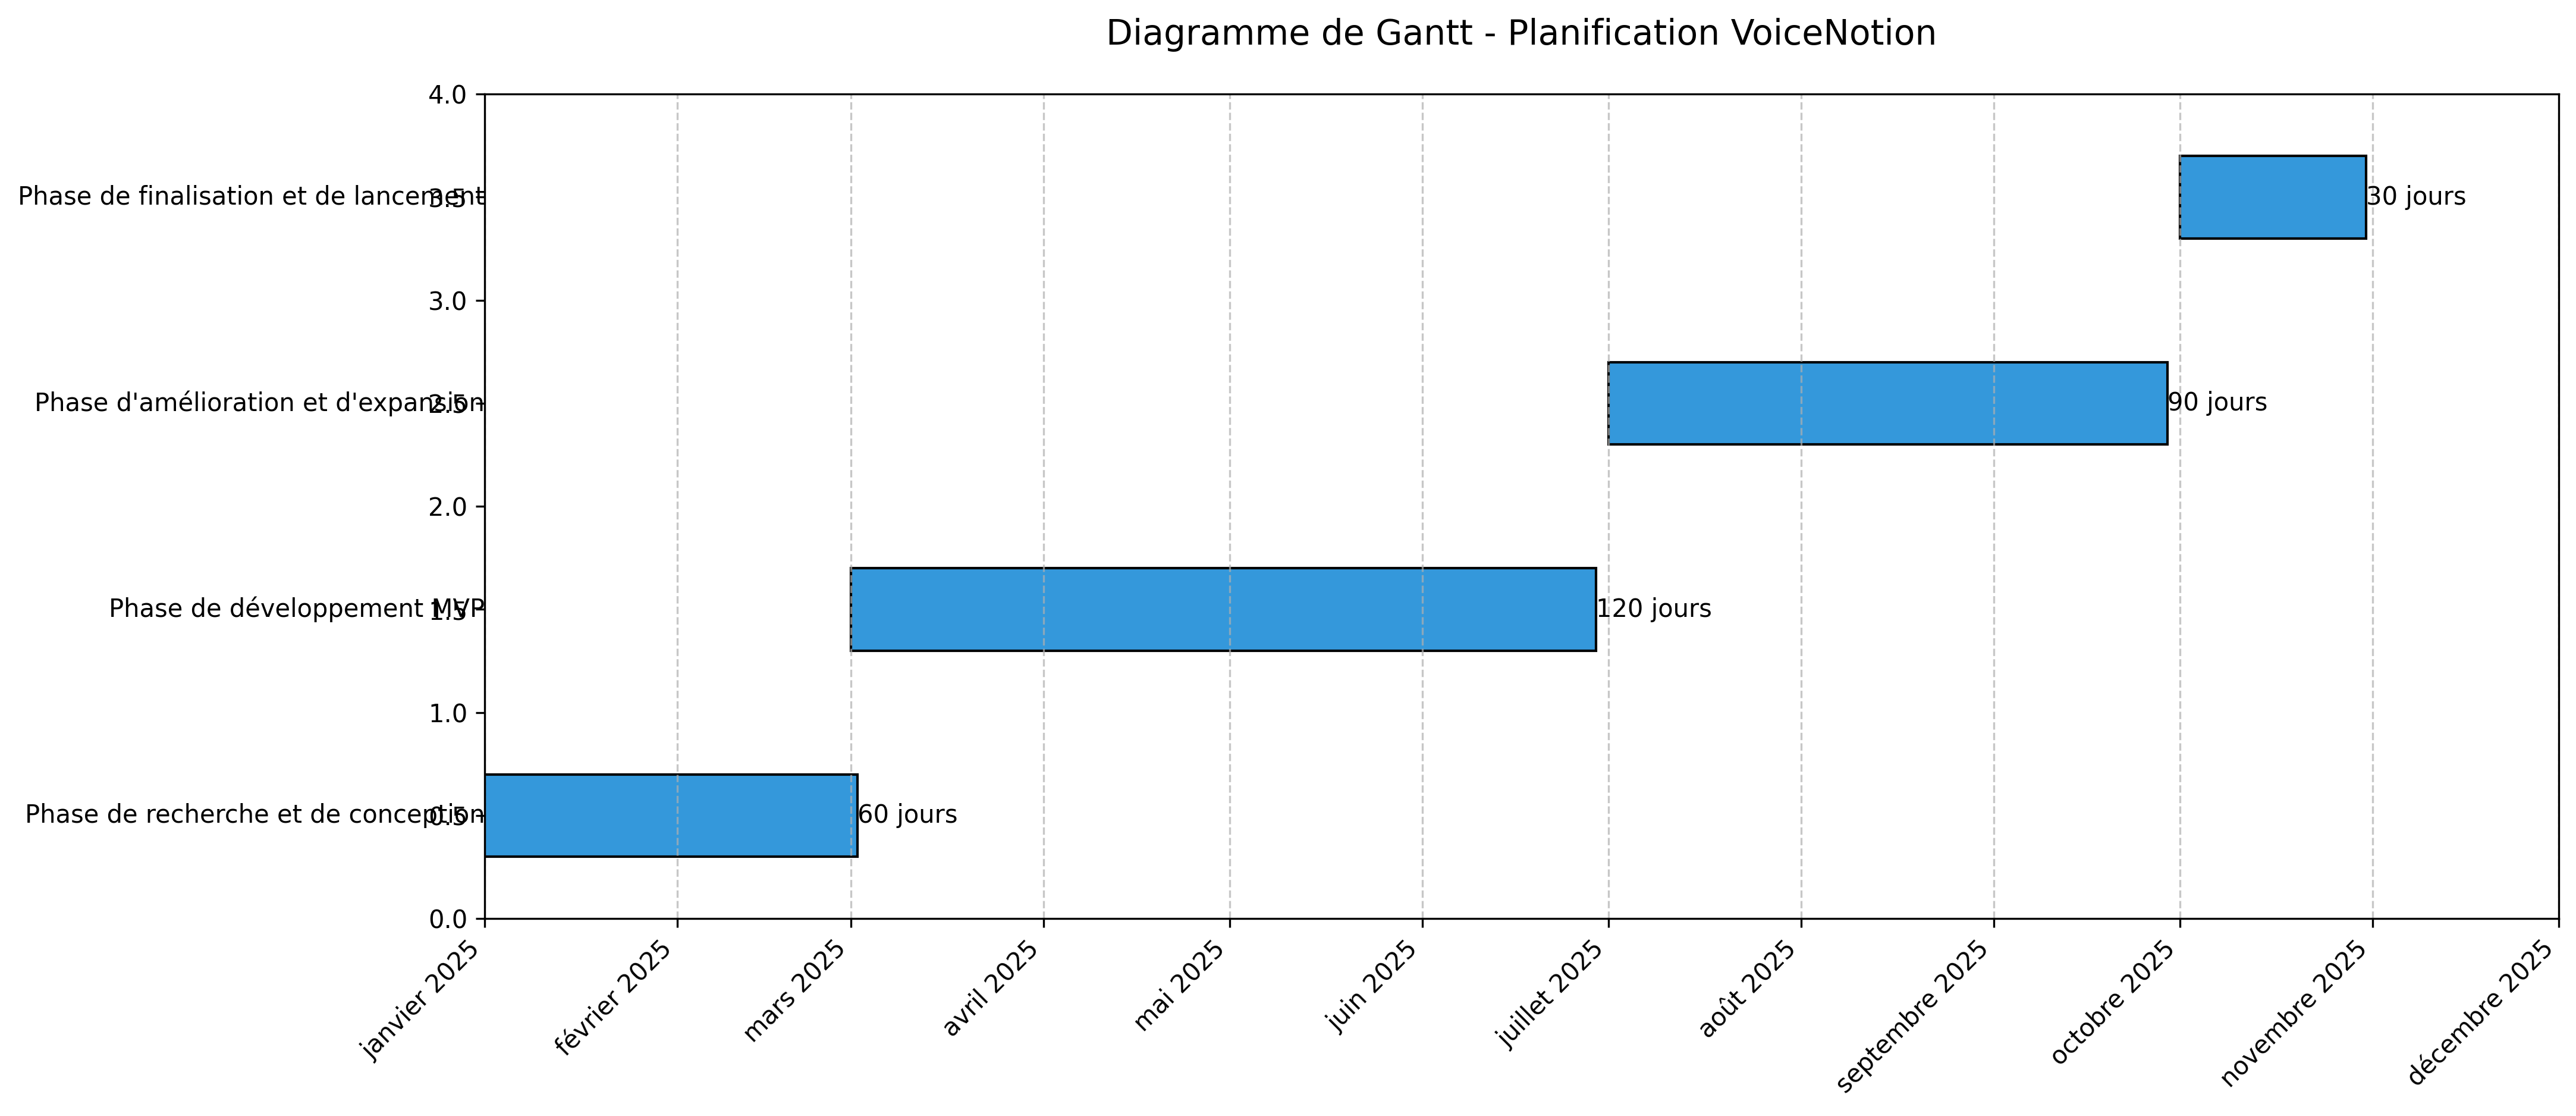
\includegraphics[width=0.9\textwidth]{assets/docs/gantt_chart.png}
        \caption{Diagramme de Gantt de planification de projet}
        \label{fig:gantt_chart}
    \end{figure}
    
    \paragraph{Calendrier détaillé (avril–juin 2025)}
Le tableau~\ref{fig:planification_table} fournit un aperçu visuel ; ci-dessous figure le même planning avec les dates exactes :

\begin{itemize}
  \item \textbf{Recherche \& planification} : 01/04/2025 – 07/04/2025
  \item \textbf{Conception graphique} : 08/04/2025 – 22/04/2025
    \begin{itemize}
      \item \textit{UI/UX Design} : 23/04/2025 – 30/04/2025
      \item \textit{Design System} : 23/04/2025 – 25/04/2025
      \item \textit{Prototypage} : 26/04/2025 – 28/04/2025
      \item \textit{Wireframing} : 29/04/2025 – 30/04/2025
      \item \textit{Animation vidéo} : 01/05/2025 – 03/05/2025
    \end{itemize}
  \item \textbf{Architecture système} : 04/05/2025 – 07/05/2025
    \begin{itemize}
      \item \textit{Conception base de données} : 08/05/2025 – 10/05/2025
    \end{itemize}
  \item \textbf{Développement \& build} : 11/05/2025 – 10/06/2025
    \begin{itemize}
      \item \textit{API (Back-End)} : 11/05/2025 – 24/05/2025
      \item \textit{Site client (Web)} : 11/05/2025 – 31/05/2025
      \item \textit{Application mobile} : 11/05/2025 – 31/05/2025
      \item \textit{Hébergement \& déploiement} : 01/06/2025 – 05/06/2025
      \item \textit{Tests} : 06/06/2025 – 10/06/2025
    \end{itemize}
  \item \textbf{Synthèse et documentation} : 11/06/2025 – 20/06/2025
    \begin{itemize}
      \item \textit{Rapport de projet} : 13/06/2025 – 17/06/2025
      \item \textit{Présentation} : 18/06/2025 – 20/06/2025
    \end{itemize}
\end{itemize}

\paragraph{Gestion des risques}
    
    Nous avons identifié plusieurs risques potentiels pour le projet et élaboré des stratégies d'atténuation:
    
    \begin{table}[H]
    \centering
    \begin{tabular}{|p{3cm}|p{5cm}|p{5cm}|}
    \hline
    \textbf{Risque} & \textbf{Impact potentiel} & \textbf{Stratégie d'atténuation} \\
    \hline
    Précision limitée de la reconnaissance vocale & Frustration utilisateur, abandon de l'application & Implémentation d'un mécanisme de correction, modes d'entrée alternatifs, tests extensifs avec différents accents \\
    \hline
    Complexité technique de l'intégration BlockNote & Retards de développement, problèmes de performance & Spike techniques précoces, exploration des alternatives, recrutement d'expertise spécifique \\
    \hline
    Expérience utilisateur non intuitive & Courbe d'apprentissage abrupte, faible adoption & Tests utilisateurs fréquents, approche itérative, tutoriels intégrés \\
    \hline
    Limites des API Gemini & Fonctionnalités restreintes, dépendance à un tiers & Plan de secours avec solutions alternatives, découplage de l'architecture \\
    \hline
    Problèmes de performance sur appareils mobiles & Lenteur, consommation excessive de batterie & Optimisation continue, tests sur différents appareils, métriques de performance \\
    \hline
    \end{tabular}
    \caption{Tableau des risques et stratégies d'atténuation}
    \label{tab:risk_management}
    \end{table}
    
    \subsection{Expérience d'utilisateur (UX)}
    
    \subsubsection{Recherche}
    
    La conception de SayNote est fondée sur une recherche approfondie pour comprendre les besoins, les attentes et les points de friction des utilisateurs potentiels en matière de prise de notes.
    
    \paragraph{Méthodologie de recherche}
    
    Notre recherche a combiné plusieurs approches:
    
    \begin{itemize}
        \item \textbf{Entretiens qualitatifs:} Nous avons mené 15 entretiens approfondis avec des utilisateurs potentiels issus de nos groupes cibles (étudiants, professionnels, créateurs de contenu).
        
        \item \textbf{Analyse concurrentielle:} Étude détaillée des applications existantes (Notion, Evernote, OneNote, Google Keep) pour identifier les forces, les faiblesses et les opportunités d'innovation.
        
        \item \textbf{Sondage en ligne:} Un questionnaire distribué à 50 participants pour quantifier les préférences et les habitudes de prise de notes.
        
        \item \textbf{Sessions d'observation:} Observation de 8 utilisateurs dans leur environnement naturel pendant qu'ils prenaient des notes, révélant des comportements et des défis non exprimés lors des entretiens.
    \end{itemize}
    
    \paragraph{Principaux insights}
    
    Cette recherche a mis en lumière plusieurs insights clés qui ont guidé notre conception:
    
    \begin{enumerate}
        \item 78\% des participants trouvent que la saisie manuelle limite leur capacité à capturer rapidement les informations lors de réunions ou de conférences.
        
        \item Les utilisateurs de Notion apprécient la flexibilité de la structure par blocs, mais 65\% trouvent la courbe d'apprentissage trop abrupte.
        
        \item 92\% des participants ont exprimé de l'intérêt pour les commandes vocales, mais 71\% craignent qu'elles ne soient pas assez précises ou intuitives.
        
        \item Les utilisateurs mobiles (81\% de notre échantillon) prennent des notes dans des contextes variés où le clavier n'est pas toujours optimal (transports, déplacements, exercice).
        
        \item La structuration post-capture est identifiée comme l'un des plus grands défis, avec 85\% des participants qui admettent ne jamais réorganiser leurs notes brutes par manque de temps.
    \end{enumerate}
    
    % Explication brève avant chaque figure
        \begin{figure}[htbp]
        \centering
        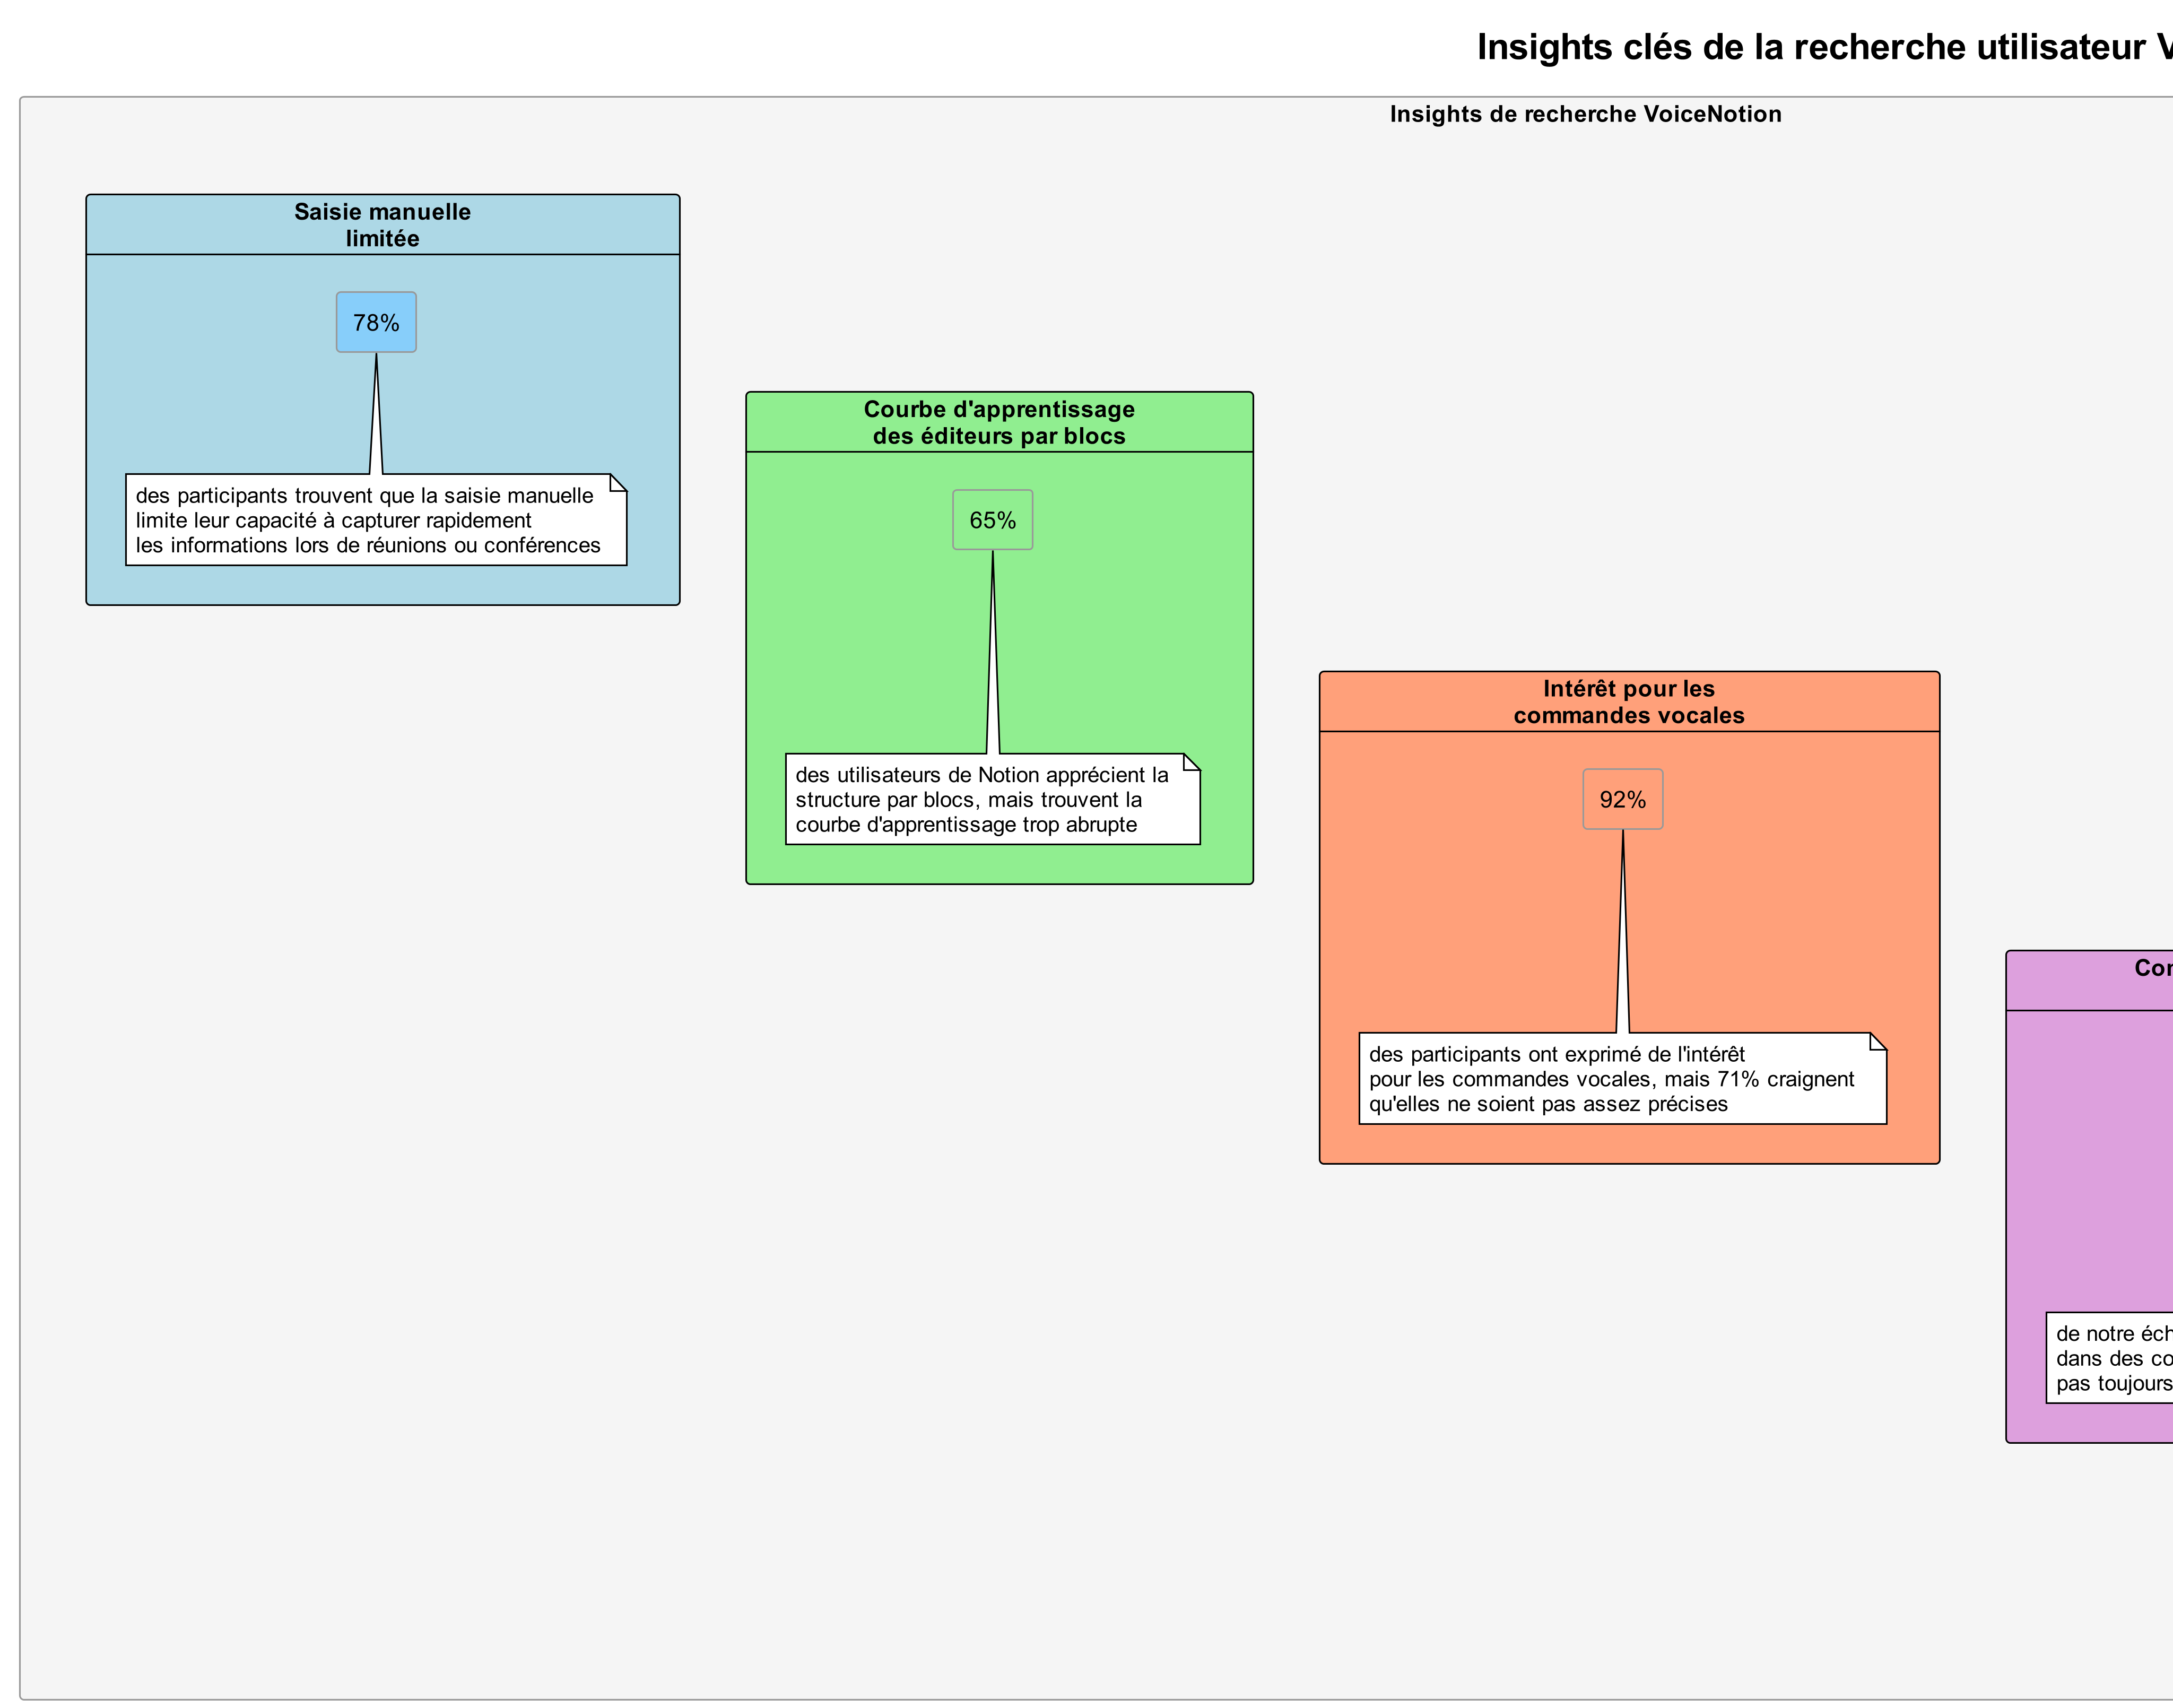
\includegraphics[width=0.75\textwidth]{assets/docs/user_research_insights.png}
        \caption{Synthèse des principaux insights de recherche utilisateur}
        \label{fig:user_research_insights}
    \end{figure}
    
    \subsubsection{Empathie}
    
    \paragraph{Personas utilisateur}
    
    Basés sur notre recherche, nous avons développé deux personas principaux qui représentent nos utilisateurs cibles:
    
    \begin{figure}[H]
        \centering
        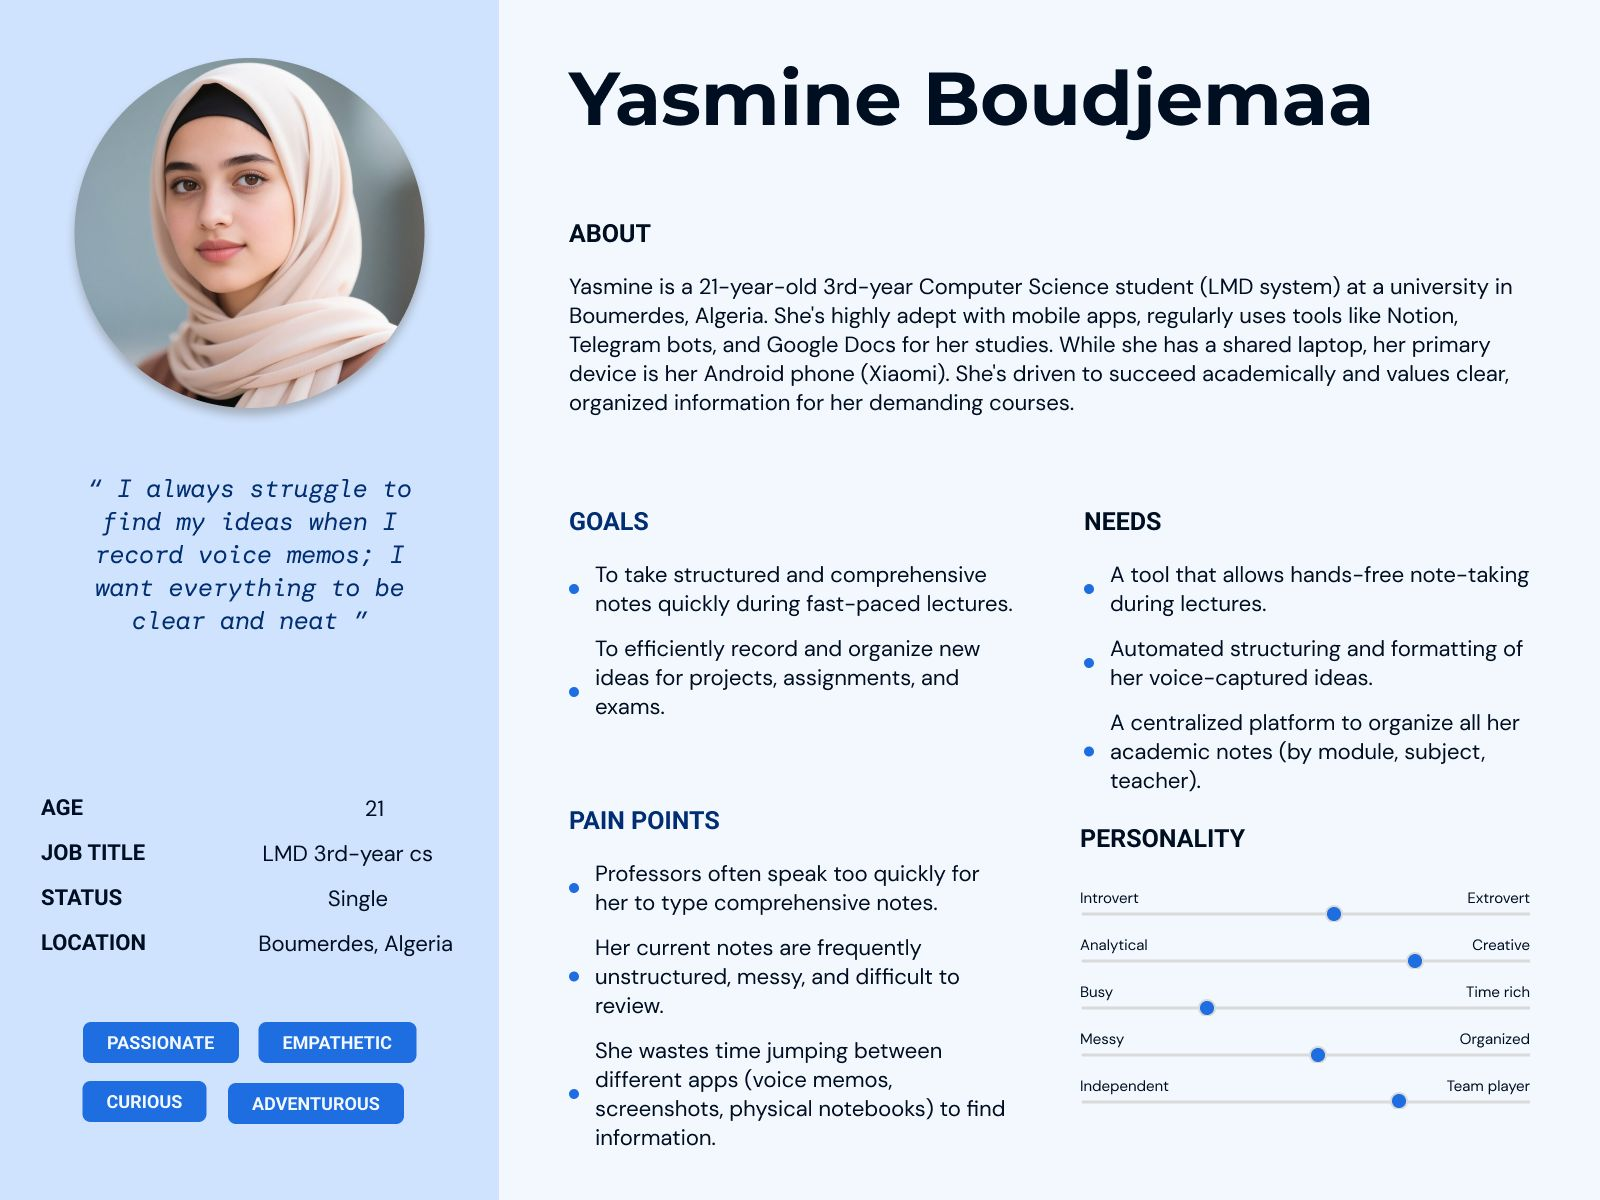
\includegraphics[width=\textwidth]{assets/docs/yassmine-personaa.jpg}
    \end{figure}
    
    \paragraph{Persona 1: Yasmine l'Étudiante en Informatique}
    
    
    \begin{itemize}
        \item \textbf{Profil:} Étudiante de 21 ans en 3ème année d'Informatique à Boumerdes. Adepte des applications mobiles (Notion, Telegram, Google Docs), elle utilise principalement son téléphone Android.
        \item \textbf{Objectifs:} Prendre des notes structurées rapidement en cours, organiser efficacement ses idées, et maintenir un système de notes propre sans réécriture manuelle.
        \item \textbf{Frustrations:} Difficulté à suivre les professeurs qui parlent vite, notes désordonnées, perte de temps entre plusieurs applications, et réorganisation manuelle fastidieuse.
        \item \textbf{Comportements:} Jongle entre mémos vocaux, captures d'écran et cahiers. Passe beaucoup de temps à réécrire et à organiser ses notes, souvent tard le soir.
        \item \textbf{Citation:} "J'ai toujours du mal à retrouver mes idées lorsque j'enregistre des mémos vocaux ; je veux que tout soit clair et bien rangé."
    \end{itemize}

    \begin{figure}[H]
        \centering
        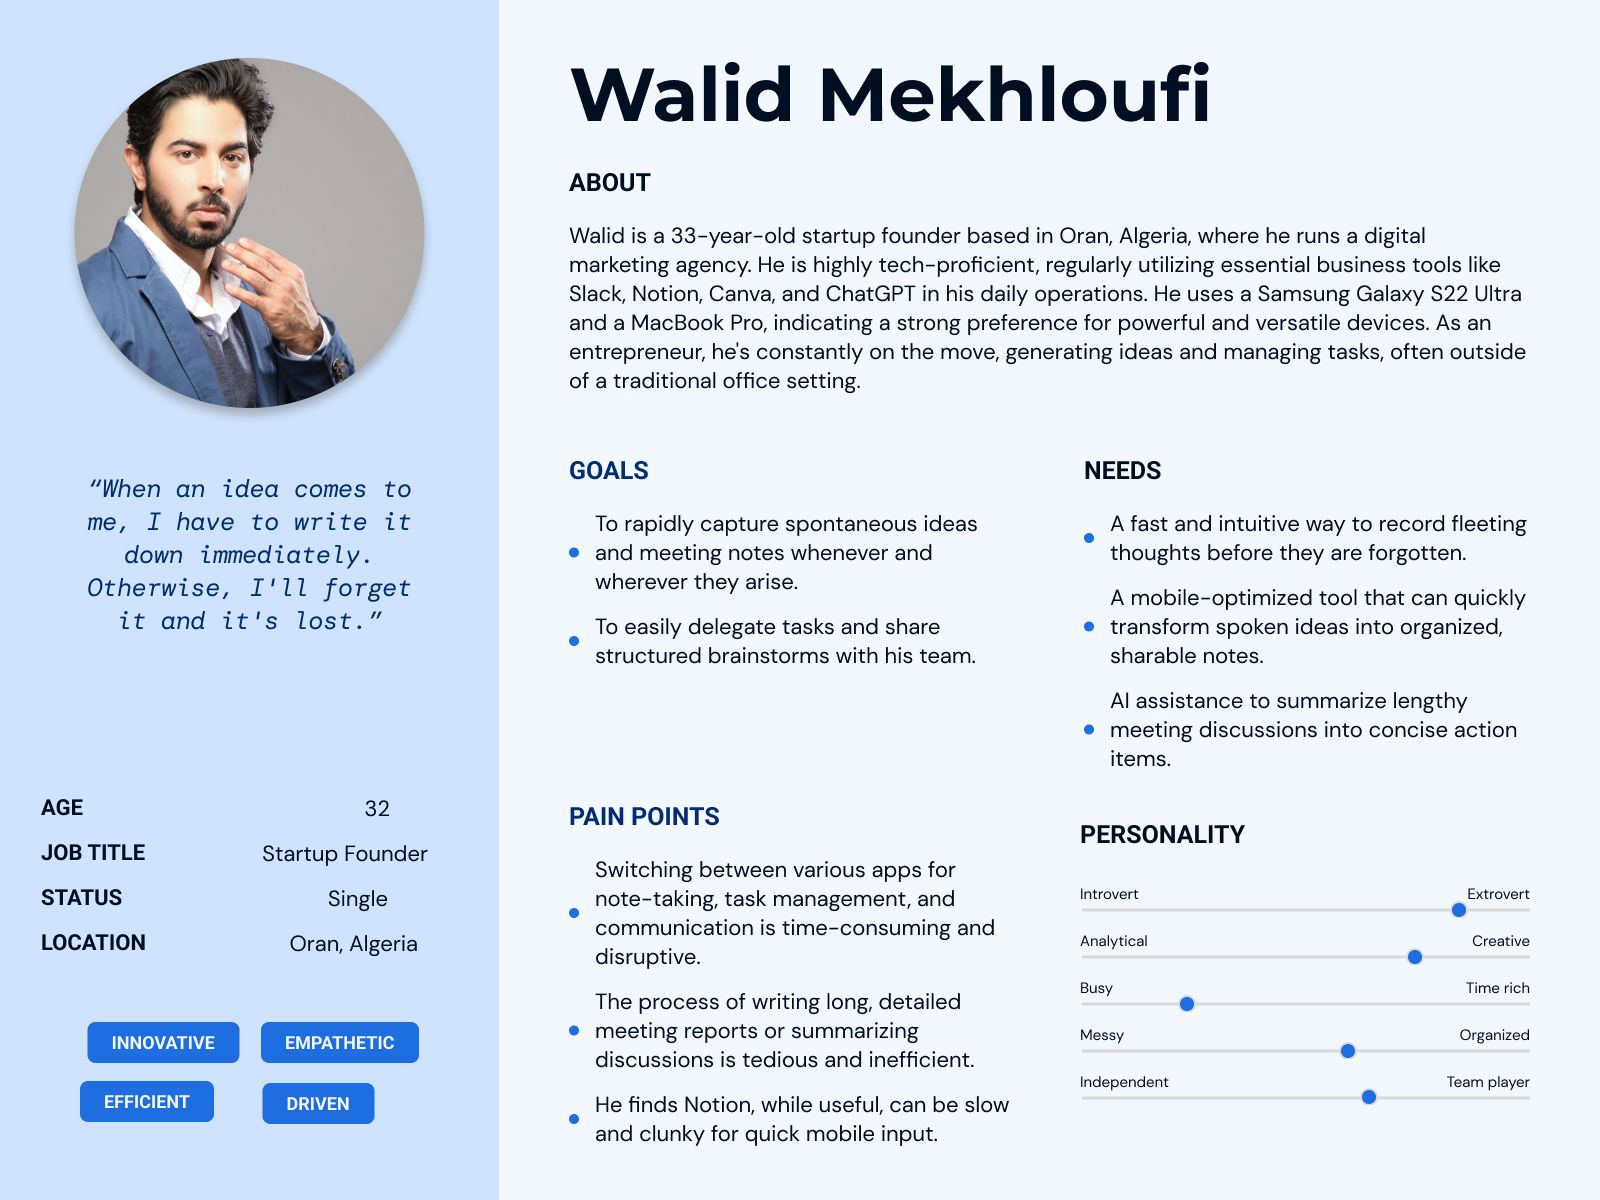
\includegraphics[width=\textwidth]{assets/docs/walid-persona.jpg}
    \end{figure}



    \paragraph{Persona 2: Walid l'Entrepreneur}

    \begin{itemize}
        \item \textbf{Profil:} Fondateur de startup de 33 ans (agence de marketing digital) à Oran. Il utilise des outils comme Slack, Notion, et ChatGPT sur son Samsung Galaxy S22 Ultra et MacBook Pro.
        \item \textbf{Objectifs:} Capturer rapidement les idées spontanées, déléguer facilement des tâches, et organiser ses idées et tâches par commandes vocales, notamment en déplacement.
        \item \textbf{Besoins:} Un moyen rapide pour enregistrer ses pensées, un outil mobile qui transforme la parole en notes structurées et partageables, et une IA pour résumer les réunions en actions concrètes.
        \item \textbf{Frustrations:} Oublie souvent des idées précieuses faute de pouvoir les noter instantanément, perd du temps à jongler entre les applications, et trouve la rédaction de comptes-rendus longue et inefficace.
        \item \textbf{Citation:} "Quand une idée me vient, je dois l’écrire direct. Sinon, je l’oublie et c’est mort."
    \end{itemize}
    
    
    % ===============================
    % Section: Wireframes et Design System
    % ===============================
    
    \subsubsection{Wireframes de l'application mobile}
    
    Avant le prototypage final, des wireframes basse fidélité ont été réalisés pour définir la structure et l'expérience utilisateur de l'application mobile SayNote.
    
    % Explication brève avant la figure
        \textit{La figure suivante présente un wireframe représentatif de l'application mobile.}
    \begin{figure}[H]
        \centering
        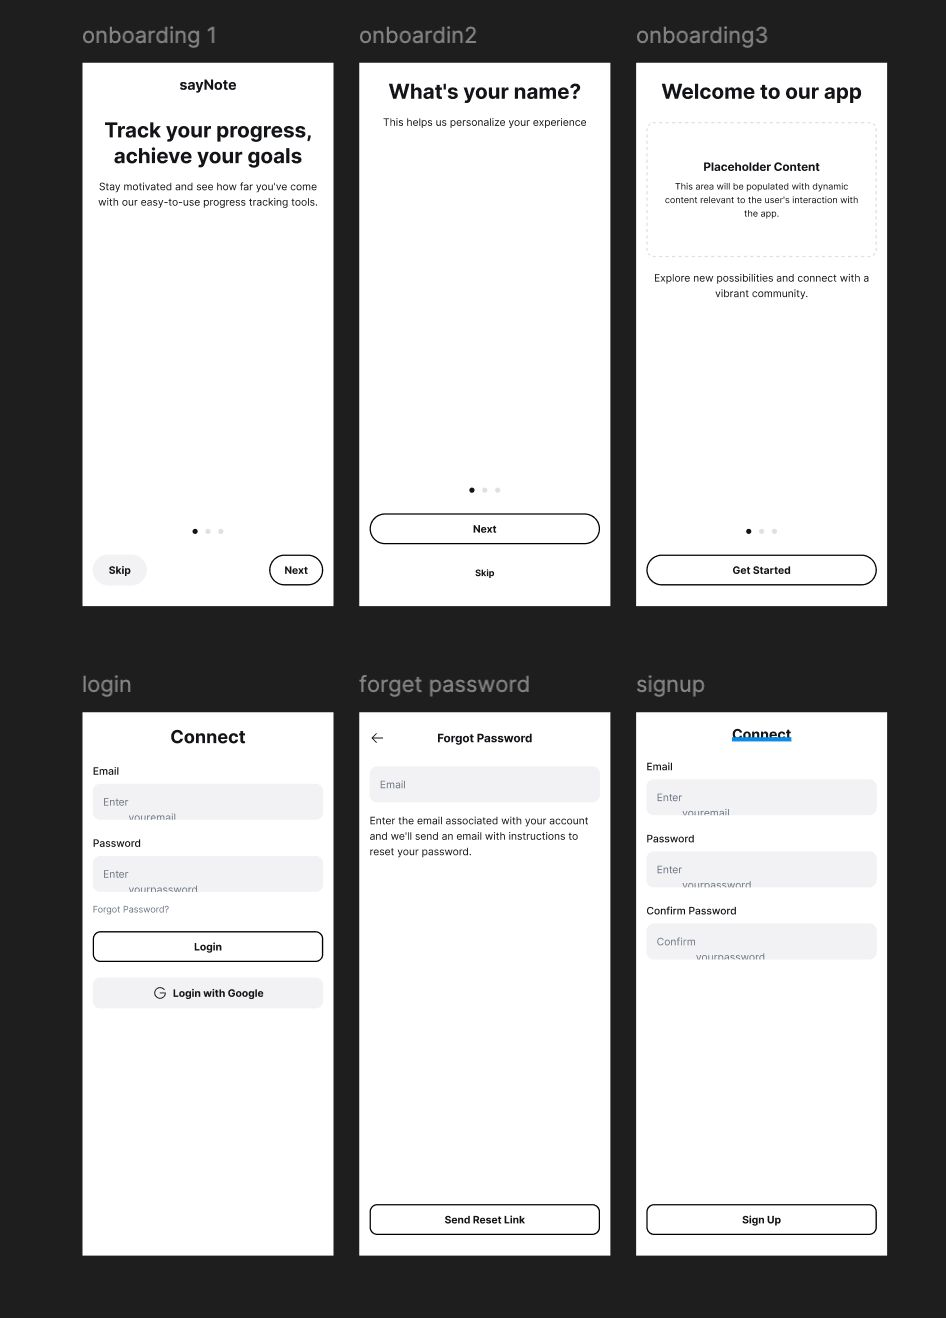
\includegraphics[width=0.9\textwidth]{assets/docs/mobile/wireframe_app-1.jpg}
        \caption{Wireframe de l'application mobile SayNote. \newline\textit{Ce schéma illustre la navigation et la disposition générale des écrans de authentification.}}
        \label{fig:wireframe_app_auth}
    \end{figure}
    
    \begin{figure}[H]
        \centering
        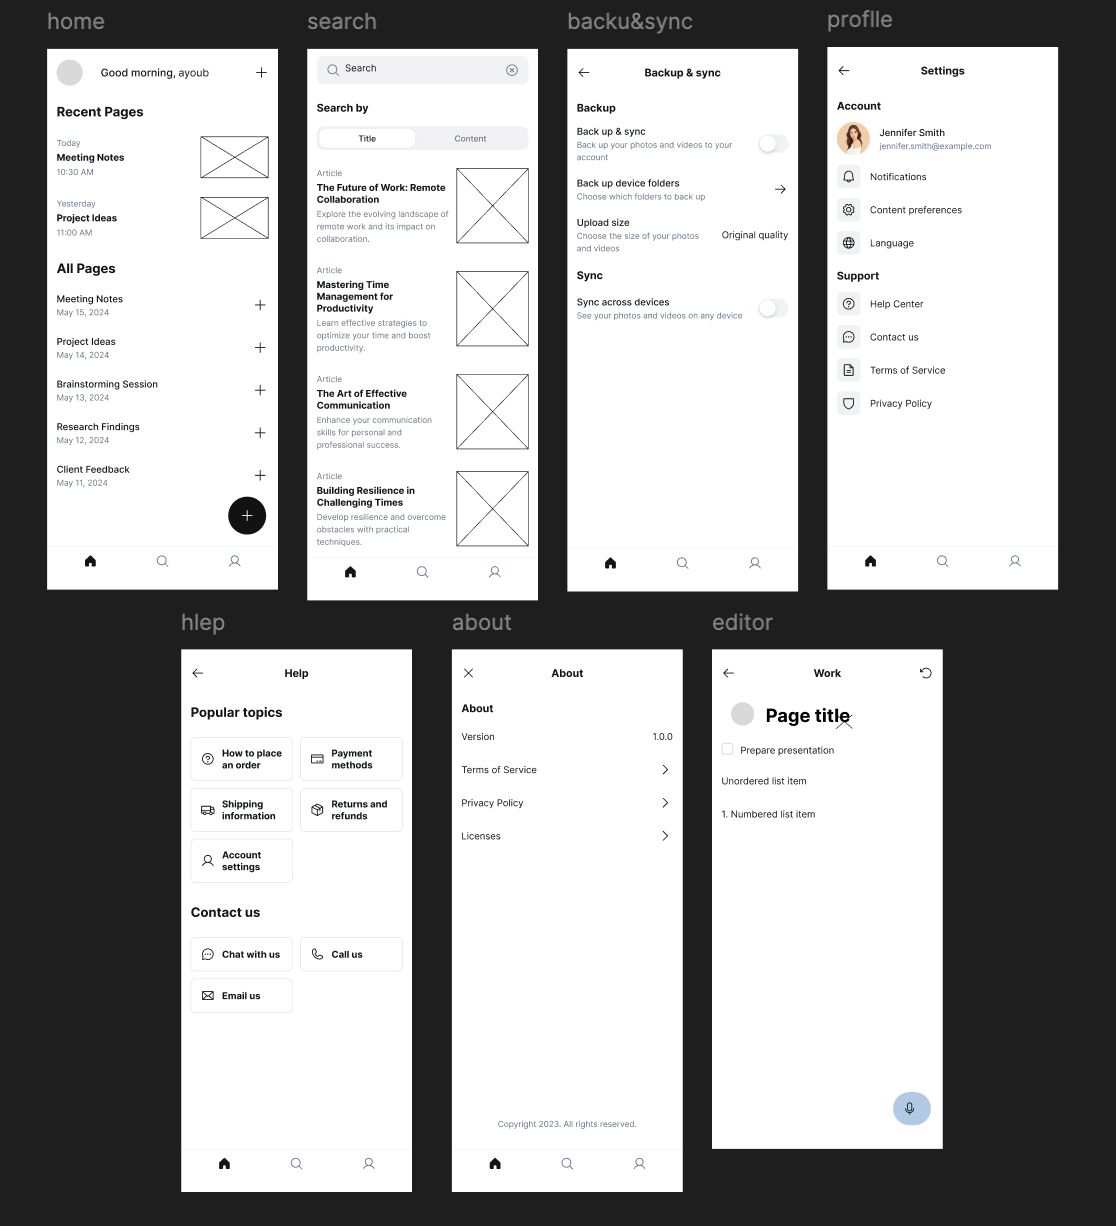
\includegraphics[width=0.9\textwidth]{assets/docs/mobile/wireframe_app-2.jpg}
        \caption{Wireframe de l'application mobile SayNote. \newline\textit{Ce schéma illustre la navigation et la disposition générale des écrans principaux.}}
        \label{fig:wireframe_app_main}
    \end{figure}
    
    
    \subsubsection{Synthèse du Design System}
    
    Une synthèse du design system a été réalisée pour garantir la cohérence visuelle et fonctionnelle de l'ensemble des interfaces.
    
        
    \paragraph{Scénarios d'utilisations}
    
    Pour chaque persona, nous avons développé des scénarios d'utilisation qui illustrent comment SayNote répondrait à leurs besoins spécifiques:
    
    \paragraph{Scénario 1: Yasmine en cours d'Algorithmique}
    
    Yasmine est en cours d'algorithmique, une matière dense où les concepts s'enchaînent rapidement.
    \begin{enumerate}
        \item Elle lance SayNote et commence à enregistrer l'audio du cours tout en tapant les points clés.
        \item Quand le professeur aborde un nouveau chapitre, elle utilise la commande vocale "Nouveau titre: Complexité des algorithmes de tri" pour structurer sa note en temps réel.
        \item Elle dit "Ajouter bloc de code" pour insérer rapidement un exemple de pseudo-code que le professeur écrit au tableau.
        \item Plus tard, en révisant, elle utilise la commande "Résumer les points clés de cette section" pour obtenir une synthèse générée par IA, ce qui lui fait gagner du temps.
        \item Elle crée une sous-page "Exercices sur les tris" directement liée à sa note de cours pour centraliser sa théorie et sa pratique.
    \end{enumerate}
    
    \paragraph{Scénario 2: Walid a une idée de campagne en voiture}
    
    Walid est en voiture entre deux rendez-vous lorsqu'une idée de campagne marketing lui vient à l'esprit.
    \begin{enumerate}
        \item Il active SayNote en mode mains libres et dit "Nouvelle idée: Campagne de fin d'année pour le client Z".
        \item Il dicte les concepts clés de la campagne: l'audience cible, le message principal et les canaux de diffusion.
        \item Il utilise la commande "Créer une liste de tâches: Actions pour l'équipe marketing" pour lister les premières étapes.
        \item Il enchaîne avec "Assigner la tâche 'étude de la concurrence' à Sarah" pour déléguer une action immédiatement.
        \item Arrivé au bureau, il ouvre la note sur son MacBook, déjà structurée, et la partage sur le canal Slack de son équipe pour discussion.
    \end{enumerate}
    
    \subsubsection{Conception du système d'information}
    
    \paragraph{Identification des acteurs}
    
    Le système SayNote interagit avec plusieurs types d'acteurs, chacun ayant des objectifs et des interactions spécifiques:
    
    \begin{itemize}
        \item \textbf{Utilisateur non authentifié:} Peut explorer la landing page, créer un compte ou se connecter.
        
        \item \textbf{Utilisateur authentifié:} Le principal acteur du système, qui peut créer, modifier, organiser et exporter des notes.
        
        \item \textbf{API Gemini:} Acteur système externe qui traite les commandes vocales et retourne des instructions structurées.
        
        \item \textbf{Service de stockage:} Acteur système responsable de la persistance et de la synchronisation des données.
    \end{itemize}
    
    \subsubsection{Diagramme de cas d'utilisation}
    
    Le diagramme de cas d'utilisation ci-dessous illustre les principales interactions entre les acteurs et le système SayNote:
    
    % Explication brève avant chaque figure
        \begin{figure}[htbp]
        \centering
        \includegraphics[width=0.9\textwidth]{assets/docs/SayNote_use_case.png}
        \caption{Diagramme de cas d'utilisation principal pour SayNote. \newline\textit{Ce diagramme UML met en évidence les interactions principales entre l'utilisateur et le système, servant de base à la conception fonctionnelle.}}
        \label{fig:use_case_diagram}
    \end{figure}
    
    Les principaux cas d'utilisation incluent:
    
    \begin{itemize}
        \item \textbf{Gestion du compte:} Inscription, connexion, modification du profil.
        
        \item \textbf{Gestion des notes:} Création, édition, suppression, création de sous-pages.
        
        \item \textbf{Interaction vocale:} Dictée de contenu, commandes de formatage, navigation par la voix.
        
        \item \textbf{Édition structurée:} Manipulation des blocs, formatage du texte, insertion d'éléments riches.
        
        \item \textbf{Recherche et filtrage:} Recherche textuelle, filtrage par date.
        
        \item \textbf{Exportation:} Export des notes vers différents formats.
    \end{itemize}
    
    \subsubsection{Diagrammes de séquence}
    
    Pour illustrer les interactions dynamiques entre l'utilisateur, l'application et les services externes, nous avons créé des diagrammes de séquence pour les processus clés.
    
    \paragraph{Séquence de commande vocale}
    
    Le diagramme suivant montre la séquence d'interactions lors de l'utilisation d'une commande vocale pour manipuler le contenu:
    
    % Explication brève avant chaque figure
        \begin{figure}[htbp]
        \centering
        \includegraphics[width=0.85\textwidth]{assets/docs/SayNote_sequence_voice.png}
        \caption{Diagramme de séquence pour le traitement d'une commande vocale. \newline\textit{Ce diagramme UML détaille le déroulement des interactions lors de l'utilisation d'une commande vocale.}}
        \label{fig:sequence_voice_command}
    \end{figure}
    
    \paragraph{Séquence de création et sauvegarde de note}
    
    Ce diagramme illustre le processus de création, d'édition et de sauvegarde d'une note:
    
    % Explication brève avant chaque figure
        \begin{figure}[htbp]
        \centering
        \includegraphics[width=0.85\textwidth]{assets/docs/SayNote_sequence_save.png}
        \caption{Diagramme de séquence pour la création et sauvegarde d'une note. \newline\textit{Ce diagramme UML montre le processus de création et de sauvegarde d'une note, mettant en évidence les interactions entre l'utilisateur et le système.}}
        \label{fig:sequence_save_note}
    \end{figure}
    
    \paragraph{Séquence d'authentification}
    
    Ce diagramme illustre le processus d'authentification des utilisateurs dans l'application:
    
    % Explication brève avant chaque figure
        \begin{figure}[htbp]
        \centering
        \includegraphics[width=0.85\textwidth]{assets/docs/SayNote_auth_sequence.png}
        \caption{Diagramme de séquence pour l'authentification. \newline\textit{Ce diagramme UML explicite les étapes de vérification et de validation lors de la connexion d'un utilisateur.}}
        \label{fig:sequence_auth}
    \end{figure}
    
    \subsubsection{Diagrammes de base de données}
    
    \paragraph{Diagramme entité-relation}
    
    Le modèle entité-relation ci-dessous représente la structure conceptuelle des données pour SayNote:
    
    % Explication brève avant chaque figure
        \begin{figure}[htbp]
        \centering
        \includegraphics[width=0.9\textwidth]{assets/docs/SayNote_er_diagram.png}
        \caption{Diagramme entité-relation pour SayNote. \newline\textit{Ce diagramme technique présente la structure conceptuelle de la base de données, essentielle pour la gestion des données.}}
        \label{fig:er_diagram}
    \end{figure}
    
    Les principales entités et leurs relations sont:
    
    \begin{itemize}
        \item \textbf{User:} Stocke les informations utilisateur (email, nom d'affichage, avatar).
        
        \item \textbf{Note:} L'entité centrale qui contient les métadonnées d'une note (titre, date de création/modification, propriétaire).
        
        \item \textbf{Block:} Représente un bloc individuel dans une note, avec son type, contenu et position.
        
        \item \textbf{Subpage:} Gère la relation hiérarchique entre les notes, permettant la création de sous-pages.
        
        \item \textbf{VoiceCommand:} Stocke les commandes vocales et leurs paramètres.
    \end{itemize}
    
    \paragraph{Diagramme de base de données}
    
    Le schéma logique de la base de données traduit le modèle entité-relation en une structure implémentable:
    
    % Explication brève avant chaque figure
        \begin{figure}[htbp]
        \centering
        \includegraphics[width=0.9\textwidth]{assets/docs/SayNote_db_schema.png}
        \caption{Schéma logique de la base de données pour SayNote. \newline\textit{Ce schéma technique traduit le modèle conceptuel en tables relationnelles pour l'implémentation.}}
        \label{fig:db_schema}
    \end{figure}
    
    Notre implémentation utilise une base de données PostgreSQL hébergée sur Supabase, avec les tables principales suivantes:
    
    \begin{itemize}
        \item \textbf{users:} id, email, display\_name, avatar\_url, created\_at, updated\_at
        
        \item \textbf{notes:} id, title, user\_id, created\_at, updated\_at, is\_archived
        
        \item \textbf{blocks:} id, note\_id, parent\_block\_id, type, content, position, created\_at, updated\_at
        
        \item \textbf{subpages:} id, parent\_note\_id, child\_note\_id, position, created\_at
        
        \item \textbf{voice\_commands:} id, user\_id, command\_text, intent\_type, parameters, created\_at
    \end{itemize}
    
    

% Chapter 3: Implementation et Developpement
\chapter{IMPLEMENTATION ET DEVELOPPEMENT}
% SayNote Implementation and Development Chapter
% Chapter 3 of the SayNote documentation

\section*{Introduction}
\addcontentsline{toc}{section}{Introduction}
Ce chapitre présente en détail l'implémentation technique de SayNote, en mettant l'accent sur l'architecture, les choix technologiques et les défis rencontrés lors du développement. Le lecteur découvrira comment les différentes composantes s'articulent pour offrir une expérience de prise de notes vocale innovante, performante et sécurisée.

Cette partie du mémoire est consacrée à l'implémentation et au développement de l'application SayNote. Nous allons détailler l'architecture technique, les technologies utilisées, et les différentes composantes de notre solution. SayNote est une application de prise de notes vocale qui combine une interface web responsive et une application mobile, toutes deux partageant une base de données commune et des fonctionnalités similaires.

Notre approche de développement a été guidée par les principes de modularité, de réutilisabilité et d'expérience utilisateur fluide. Nous avons adopté des technologies modernes pour garantir la performance, la sécurité et l'évolutivité de notre solution.

\section{Architecture globale}
L'architecture de SayNote est construite autour d'une approche multi-plateforme avec un backend commun. Cette architecture permet de maintenir une expérience utilisateur cohérente tout en optimisant le développement pour chaque plateforme.

\begin{figure}[H]
    \centering
    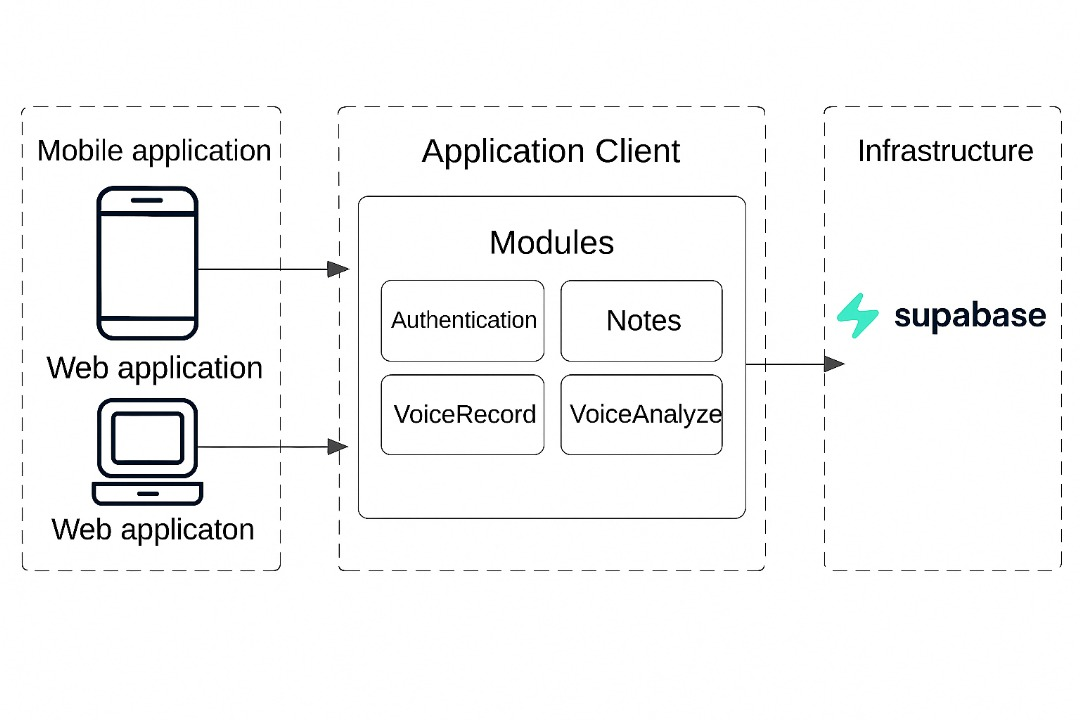
\includegraphics[width=0.8\textwidth]{assets/docs/golobal-diagrams/global-architecture.jpg}
    \caption{Architecture globale de SayNote}
    \label{fig:global-architecture}
\end{figure}

\subsection{Composants principaux}
\begin{itemize}
    \item \textbf{Application Web}: Développée avec Next.js\resref{res:nextjs} et React, offrant une interface responsive et optimisée pour les navigateurs desktop et mobiles.
    \item \textbf{Application Mobile}: Construite avec React Native\resref{res:reactnative} et Expo\resref{res:expo}, permettant un déploiement natif sur iOS et Android.
    \item \textbf{Backend}: Utilisant Supabase\resref{res:supabase} comme solution Backend-as-a-Service (BaaS) pour l'authentification, la base de données, et le stockage.
    \item \textbf{API Gemini}: Intégration de l'API Gemini de Google pour la reconnaissance vocale et le traitement des commandes.
\end{itemize}

\subsection{Flux de données}
Le flux de données dans SayNote suit un modèle client-serveur avec synchronisation en temps réel:
\begin{enumerate}
    \item L'utilisateur interagit avec l'application (web ou mobile)
    \item Les requêtes sont envoyées au backend Supabase\resref{res:supabase} via des API sécurisées
    \item Les données sont stockées dans une base de données PostgreSQL\resref{res:postgresql}
    \item Les mises à jour sont synchronisées en temps réel entre les appareils grâce aux abonnements Supabase\resref{res:supabase}
\end{enumerate}

\section{Environnement de developpement}
\subsection{Materiels}
Le developpement de SayNote a ete realise sur les equipements suivants:
\begin{itemize}
    \item MacBook Pro M1 (16GB RAM, 512GB SSD)
    \item iPhone 13 Pro (pour les tests iOS)
    \item Samsung Galaxy S21 (pour les tests Android)
    \item iPad Pro (pour les tests de la version tablette)
\end{itemize}

\subsection{Logiciels et outils de developpement}

\subsubsection{Visual Studio Code}
\begin{wrapfigure}{r}{0.3\textwidth}
    \centering
    
\includegraphics[width=0.25\textwidth]{assets/docs/vscode.png}
\end{wrapfigure}
Visual Studio Code est un editeur de code source leger mais puissant qui s'execute sur votre bureau et est disponible pour Windows, macOS et Linux. Il est fourni avec un support integre pour JavaScript, TypeScript\resref{res:typescript} et Node.js et dispose d'un riche ecosysteme d'extensions pour d'autres langages et environnements de developpement.

Visual Studio Code a ete notre IDE principal pour le developpement de SayNote. Nous avons utilise plusieurs extensions pour ameliorer notre productivite:

\begin{itemize}
    \item ESLint\resref{res:eslint}: Pour la verification du code JavaScript/TypeScript\resref{res:typescript}
    \item Prettier\resref{res:prettier}: Pour le formatage automatique du code
    \item React Developer Tools: Pour le debogage des composants React
    \item Tailwind CSS IntelliSense\resref{res:tailwind}: Pour l'autocompletion des classes Tailwind
    \item GitLens: Pour une meilleure integration avec Git
\end{itemize}

\subsubsection{GitHub}
\begin{wrapfigure}{r}{0.3\textwidth}
    \centering
    
\includegraphics[width=0.25\textwidth]{assets/docs/github.png}
\end{wrapfigure}
GitHub est une plateforme de developpement collaboratif basee sur Git, un systeme de controle de version distribue. Il est largement utilise par les developpeurs pour heberger, gerer et partager des projets de developpement de logiciels.

Sur GitHub, les developpeurs peuvent creer des depots pour stocker leur code source, collaborer avec d'autres developpeurs sur des projets, suivre et gerer les problemes, et faciliter le processus de developpement via des fonctionnalites comme les pull requests, les actions, et plus encore.

Pour SayNote, nous avons utilise GitHub pour:
\begin{itemize}
    \item Gestion du code source avec branches pour chaque fonctionnalite
    \item Organisation du travail d'equipe via les issues et les projets
    \item Integration continue avec GitHub Actions\resref{res:githubactions}
    \item Revue de code via les pull requests
    \item Documentation du projet dans le wiki et le README
\end{itemize}



\subsubsection{Zod}
\begin{wrapfigure}{r}{0.3\textwidth}
    \centering
    
\includegraphics[width=0.25\textwidth]{assets/docs/logo_zod.png}
\end{wrapfigure}
Zod est une bibliotheque de validation de schemas axee sur TypeScript\resref{res:typescript}. Elle offre une API puissante et expressive pour definir et valider des schemas de donnees. 

Avec Zod, nous pouvons facilement definir des regles de validation complexes pour differents types de donnees tels que les chaines de caracteres, les nombres, les tableaux, les objets, et bien d'autres. Il prend en charge des fonctionnalites avancees telles que la validation conditionnelle, les messages d'erreur personnalises et la composition de schemas.

Zod favorise le typage fort et l'inference de types, ce qui en fait un choix ideal pour les projets TypeScript\resref{res:typescript}. Il s'integre egalement parfaitement avec des frameworks et des bibliotheques populaires comme React et Express. 

Dans SayNote, nous utilisons Zod pour:
\begin{itemize}
    \item Valider les donnees des formulaires utilisateur
    \item Verifier l'integrite des donnees provenant de l'API
    \item Generer des types TypeScript\resref{res:typescript} a partir des schemas de validation
    \item Assurer la coherence des donnees entre le frontend et le backend
\end{itemize}

\subsubsection{Tests}
\begin{wrapfigure}{r}{0.3\textwidth}
    \centering
    
\includegraphics[width=0.25\textwidth]{assets/docs/jest.png}\\
    \vspace{0.5cm}
    
\includegraphics[width=0.25\textwidth]{assets/docs/cypress.png}
\end{wrapfigure}
Pour assurer la qualite et la fiabilite de notre application, nous avons mis en place une strategie de tests complete avec Jest\resref{res:jest} et Cypress\resref{res:cypress}.

\textbf{Jest\resref{res:jest}} est un framework de test JavaScript concu pour assurer la correction de n'importe quel code JavaScript. Jest\resref{res:jest} est complet et facile a configurer, et nous l'avons utilise pour les tests unitaires et d'integration.

\textbf{Cypress\resref{res:cypress}} est un framework de test end-to-end qui nous permet de tester notre application comme le ferait un utilisateur reel. Il offre une experience de test fiable, rapide et facile a comprendre.

Notre approche de test comprend:
\begin{itemize}
    \item Tests unitaires pour les fonctions et composants individuels
    \item Tests d'integration pour verifier les interactions entre composants
    \item Tests end-to-end pour simuler les parcours utilisateur complets
    \item Tests d'accessibilite pour garantir que l'application est utilisable par tous
\end{itemize}

\section{Outils de conception et design}

\subsection{Figma}
\begin{wrapfigure}{r}{0.3\textwidth}
    \centering
    
\includegraphics[width=0.25\textwidth]{assets/docs/figma.png}
\end{wrapfigure}
Figma est un outil de conception d'interface utilisateur base sur le cloud qui permet aux equipes de collaborer en temps reel. Il est devenu notre outil principal pour la conception de l'interface utilisateur et la creation de prototypes interactifs. Il nous a permis de:

\begin{itemize}
    \item Creer des wireframes et des maquettes haute fidelite
    \item Concevoir un systeme de design coherent avec des composants reutilisables
    \item Collaborer en temps reel sur les designs
    \item Tester les interactions via des prototypes cliquables
    \item Generer des specifications pour les developpeurs
\end{itemize}

L'interface intuitive de Figma et ses fonctionnalites avancees ont grandement facilite le processus de conception, permettant a notre equipe de travailler efficacement meme a distance.
\subsection{Adobe Illustrator}
\begin{wrapfigure}{r}{0.3\textwidth}
    \centering
    
\includegraphics[width=0.25\textwidth]{assets/docs/illustrator.png}
\end{wrapfigure}
Adobe Illustrator est un logiciel de creation graphique et de dessin vectoriel largement utilise dans l'industrie du design. Il offre un large eventail d'outils et de fonctionnalites qui permettent de creer des illustrations, des logos, des icones, des graphiques et d'autres elements visuels de haute qualite. 

Illustrator utilise des vecteurs pour creer des images, ce qui signifie que les dessins peuvent etre redimensionnes et modifies sans perte de qualite. Il prend en charge la creation de formes, le trace de courbes, l'application de couleurs et de degrades, la manipulation des calques et bien plus encore.

Nous avons utilise Adobe Illustrator pour creer les elements graphiques vectoriels de notre identite visuelle:

\begin{itemize}
    \item Logo SayNote et ses variantes
    \item Icones personnalisees
    \item Illustrations pour le site web et l'application
    \item Materiel marketing (bannieres, visuels pour reseaux sociaux)
\end{itemize}

% Explication brève avant chaque figure
\noindent
\textit{La figure suivante illustre la creation des elements graphiques avec Adobe Illustrator}
\begin{figure}[H]
\centering
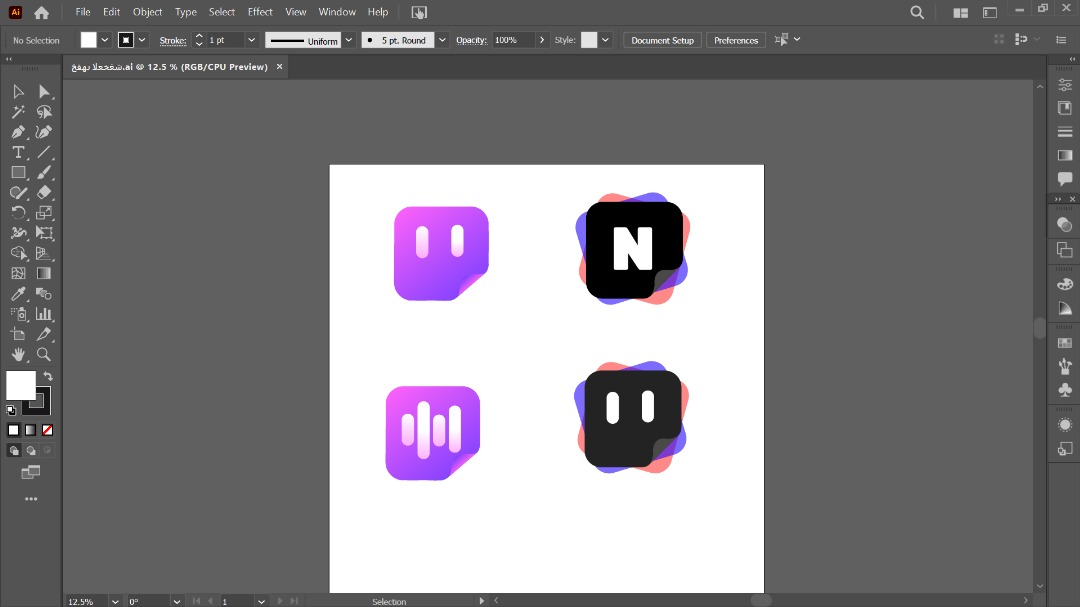
\includegraphics[width=0.8\textwidth]{assets/docs/working-ulistrator.jpg}
\caption{Creation des elements graphiques avec Adobe Illustrator}
\label{fig:illustrator-assets}
\end{figure}

\subsection{Adobe Photoshop}
\begin{wrapfigure}{r}{0.3\textwidth}
    \centering
    
\includegraphics[width=0.25\textwidth]{assets/docs/photoshop.png}
\end{wrapfigure}
Adobe Photoshop est un logiciel de retouche d'image et de creation graphique largement utilise dans le domaine de la conception, de la photographie et du multimedia. Il offre une gamme complete d'outils et de fonctionnalites avances pour manipuler et ameliorer les images.

Avec Photoshop, nous avons effectue des retouches precises, ajuste la luminosite et le contraste, corrige les couleurs, supprime des objets indesirables, et cree des compositions complexes pour notre application. Cet outil nous a ete particulierement utile pour:

\begin{itemize}
    \item Retoucher les captures d'ecran de l'application
    \item Creer des mockups realistes pour presentations
    \item Preparer des images optimisees pour le web et les applications mobiles
    \item Creer des elements graphiques complexes combines avec Illustrator
\end{itemize}

\section{Backend et services cloud}

\subsection{Supabase\resref{res:supabase}}
\begin{wrapfigure}{r}{0.3\textwidth}
    \centering
    
\includegraphics[width=0.25\textwidth]{assets/docs/logo_supabase.png}
\end{wrapfigure}
Supabase\resref{res:supabase} est une solution Backend-as-a-Service (BaaS) open-source qui offre une alternative a Firebase. Cette plateforme nous offre:

\begin{itemize}
    \item Une base de donnees PostgreSQL\resref{res:postgresql} performante et evolutive
    \item Un systeme d'authentification securise avec plusieurs methodes de connexion
    \item Des API RESTful et GraphQL generees automatiquement
    \item Des fonctionnalites de temps reel pour la synchronisation des donnees
    \item Un stockage de fichiers integre
\end{itemize}

Nous avons choisi Supabase\resref{res:supabase} pour sa flexibilite, sa scalabilite et sa compatibilite avec PostgreSQL\resref{res:postgresql}, ce qui nous permet de beneficier d'une base de donnees relationnelle complete sans avoir a gerer l'infrastructure sous-jacente. L'authentification integree et les fonctionnalites en temps reel ont egalement considerablement accelere notre developpement.

Avec Supabase\resref{res:supabase}, nous avons pu implementer rapidement des fonctionnalites essentielles comme la synchronisation des notes entre appareils, la gestion des utilisateurs et le stockage des fichiers multimedia associes aux notes.

% Explication brève avant chaque figure
\noindent
\textit{La figure suivante illustre les fonctionnalites principales de Supabase\resref{res:supabase} pour SayNote}
\begin{figure}[H]
\centering
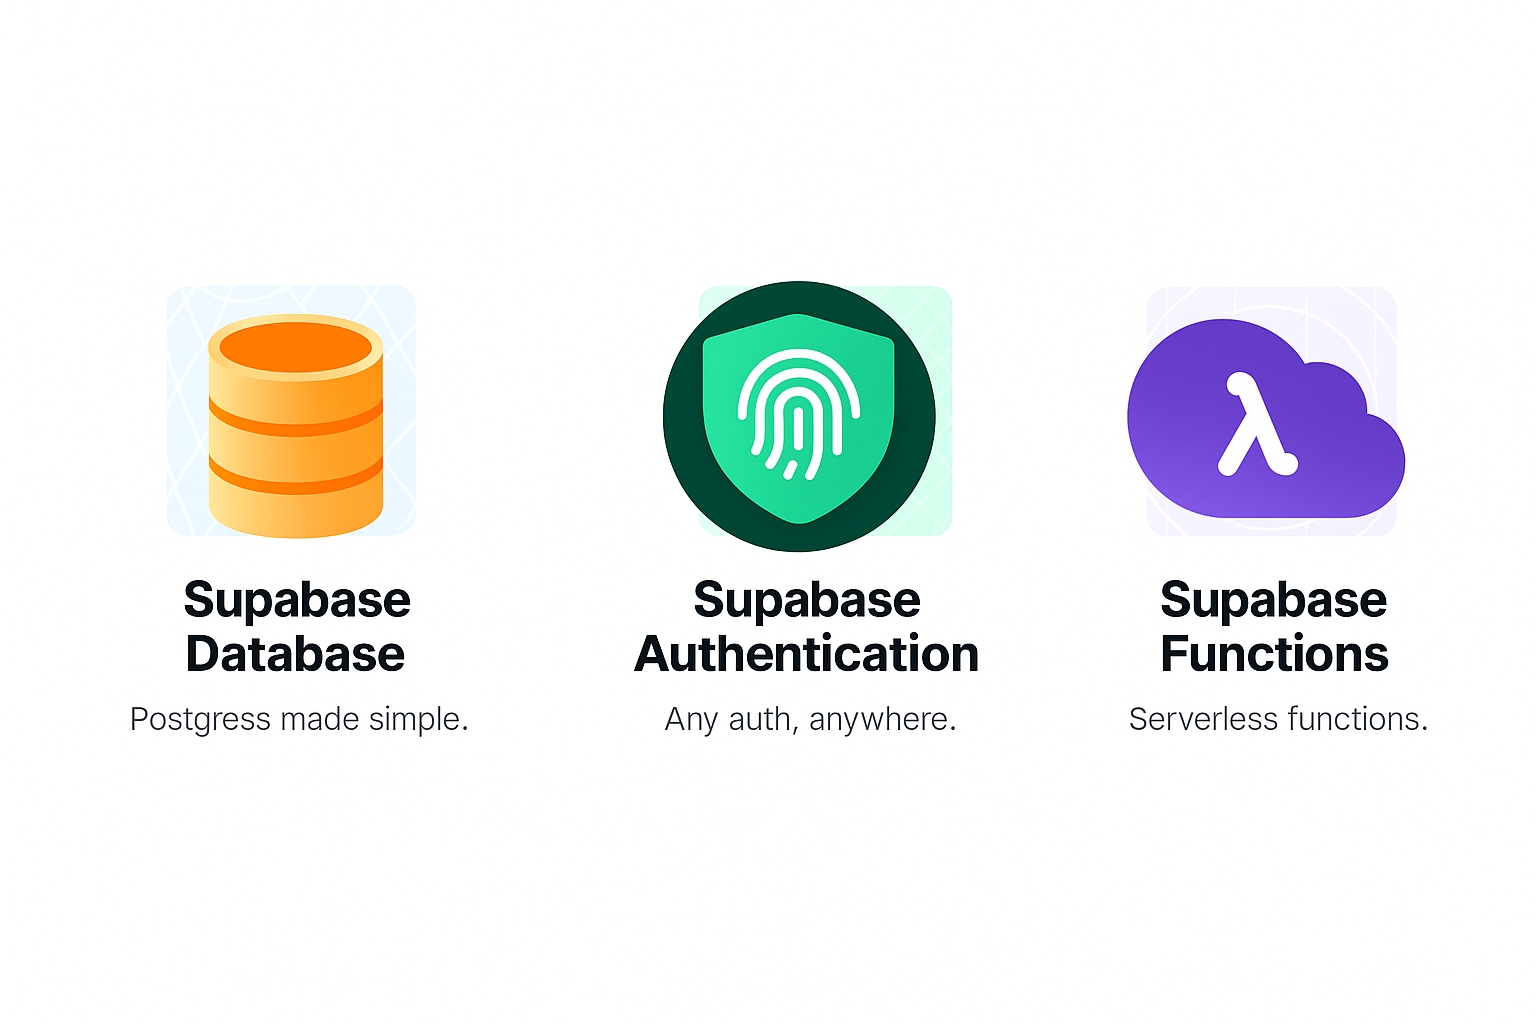
\includegraphics[width=0.8\textwidth]{assets/docs/golobal-diagrams/supabase-feature.png}
\caption{Fonctionnalites principales de Supabase\resref{res:supabase} pour SayNote}
\label{fig:supabase-feature}
\end{figure}


\subsection{Authentification avec Supabase\resref{res:supabase}}

Supabase\resref{res:supabase} fournit une solution d'authentification complète et facile à intégrer. Elle prend en charge une variété de méthodes d'authentification, y compris l'email et le mot de passe, les fournisseurs OAuth (comme Google, GitHub, etc.), et les liens magiques.

Pour SayNote, nous avons utilisé l'authentification par email et mot de passe de Supabase\resref{res:supabase} pour sécuriser l'accès des utilisateurs. Le processus est simple :
\begin{itemize}
    \item \textbf{Inscription (Sign Up):} Un nouvel utilisateur crée un compte avec son adresse email et un mot de passe. Supabase\resref{res:supabase} gère la création de l'utilisateur dans sa base de données d'authentification et envoie un email de confirmation.
    \item \textbf{Connexion (Sign In):} Un utilisateur existant se connecte avec ses identifiants. Supabase\resref{res:supabase} vérifie les informations et, en cas de succès, renvoie un JSON Web Token (JWT).
    \item \textbf{Gestion de session:} Le JWT est utilisé pour authentifier les requêtes API ultérieures, permettant à l'utilisateur d'accéder aux ressources protégées. Supabase\resref{res:supabase} gère automatiquement le rafraîchissement des tokens pour maintenir la session active.
\end{itemize}

Cette approche nous a permis de mettre en place un système d'authentification robuste et sécurisé rapidement, sans avoir à gérer la complexité de l'infrastructure sous-jacente.

\begin{figure}[H]
\centering
\end{figure}


\vspace{10em} 
\captionof{figure}{Composant d'authentification}
\label{fig:auth-component}
\begin{lstlisting}[breaklines=true]
// components/AuthForm.tsx
"use client";

import { useState } from "react";
import { supabase } from "@/lib/supabase";
import { Button } from "@/components/ui/Button";
import { Input } from "@/components/ui/Input";

export default function AuthForm({ mode = "login" }) {
  const [email, setEmail] = useState("");
  const [password, setPassword] = useState("");
  const [loading, setLoading] = useState(false);
  const [error, setError] = useState("");
  
  const handleSubmit = async (e) => {
    e.preventDefault();
    setLoading(true);
    setError("");
    
    try {
      if (mode === "login") {
        const { error } = await supabase.auth.signInWithPassword({
          email,
          password,
        });
        if (error) throw error;
      } else {
        const { error } = await supabase.auth.signUp({
          email,
          password,
        });
        if (error) throw error;
      }
    } catch (error) {
      setError(error.message);
    } finally {
      setLoading(false);
    }
  };
  
  return (
    <form onSubmit={handleSubmit} className="space-y-4">
      {error && <div className="p-3 bg-red-100 text-red-700 rounded">{error}</div>}
      
      <div>
        <label htmlFor="email" className="block text-sm font-medium">
          Email
        </label>
        <Input
          id="email"
          type="email"
          value={email}
          onChange={(e) => setEmail(e.target.value)}
          required
        />
      </div>
      
      <div>
        <label htmlFor="password" className="block text-sm font-medium">
          Mot de passe
        </label>
        <Input
          id="password"
          type="password"
          value={password}
          onChange={(e) => setPassword(e.target.value)}
          required
        />
      </div>
      
      <Button type="submit" primary disabled={loading}>
        {loading 
          ? "Chargement..." 
          : mode === "login" ? "Se connecter" : "S'inscrire"}
      </Button>
    </form>
  );
}
\end{lstlisting}


\section{Application mobile}
\subsection{Technologies et outils utilises}

\subsubsection{React Native\resref{res:reactnative}}
\begin{minipage}{0.7\textwidth}
React Native\resref{res:reactnative} est un framework de developpement d'applications mobiles cree par Facebook (Meta) qui permet de construire des applications natives pour Android et iOS a partir d'une base de code JavaScript/React commune. Il offre une approche "apprendre une fois, ecrire partout" pour le developpement mobile.

Les principales caracteristiques de React Native\resref{res:reactnative} qui ont guide notre choix pour SayNote sont:

\begin{itemize}
    \item \textbf{Composants natifs}: React Native\resref{res:reactnative} compile le code JavaScript en composants natifs, offrant des performances proches des applications natives
    \item \textbf{Partage de code}: Possibilite de partager une grande partie du code entre les plateformes iOS et Android
    \item \textbf{Hot Reloading}: Visualisation instantanee des modifications du code pendant le developpement
    \item \textbf{Communaute active}: Large ecosysteme de bibliotheques et support communautaire
    \item \textbf{Approche declarative}: Interface utilisateur construite de maniere declarative, similaire a React
\end{itemize}

React Native\resref{res:reactnative} nous a permis de developper l'application mobile SayNote pour iOS et Android a partir d'une seule base de code, tout en offrant une experience utilisateur native et performante sur chaque plateforme.
\end{minipage}%
\hfill
\begin{minipage}{0.25\textwidth}
\centering

\includegraphics[width=0.9\textwidth]{assets/docs/logo_reactnative.png}
\end{minipage}

\begin{codebox}{Configuration du projet React Native\resref{res:reactnative}}
\begin{lstlisting}
// app.json
{
  "expo": {
    "name": "SayNote",
    "slug": "SayNote",
    "version": "1.0.0",
    "orientation": "portrait",
    "icon": "./assets/icon.png",
    "userInterfaceStyle": "light",
    "splash": {
      "image": "./assets/splash.png",
      "resizeMode": "contain",
      "backgroundColor": "#ffffff"
    },
    "assetBundlePatterns": ["**/*"],
    "ios": {
      "supportsTablet": true,
      "bundleIdentifier": "com.SayNote.app"
    },
    "android": {
      "adaptiveIcon": {
        "foregroundImage": "./assets/adaptive-icon.png",
        "backgroundColor": "#ffffff"
      },
      "package": "com.SayNote.app"
    },
    "plugins": [
      [
        "expo-av",
        {
          "microphonePermission": "Autoriser SayNote a acceder a votre microphone."
        }
      ]
    ]
  }
}
\end{lstlisting}
\end{codebox}

\subsubsection{Expo\resref{res:expo}}
\begin{minipage}{0.7\textwidth}
Expo\resref{res:expo} est une plateforme et un ensemble d'outils construits autour de React Native\resref{res:reactnative} qui simplifient considerablement le developpement, le test et le deploiement d'applications mobiles. Il offre une approche "batteries included" pour React Native\resref{res:reactnative}.

Les avantages d'Expo\resref{res:expo} qui ont guide notre choix pour SayNote sont:

\begin{itemize}
    \item \textbf{Configuration simplifiee}: Pas besoin de configurer manuellement le SDK natif d'Android ou iOS
    \item \textbf{Modules preintegres}: Acces a des APIs natives courantes (camera, geolocalisation, etc.) via des modules preconfiguress
    \item \textbf{Expo\resref{res:expo} Go}: Application de test qui permet de visualiser les changements en temps reel sur des appareils physiques
    \item \textbf{EAS (Expo\resref{res:expo} Application Services)}: Services de build, deploiement et mise a jour des applications
    \item \textbf{Over-the-air updates}: Possibilite de deployer des mises a jour sans passer par les App Stores
\end{itemize}

Expo\resref{res:expo} nous a permis d'accelerer considerablement le developpement de l'application mobile SayNote, en simplifiant l'acces aux fonctionnalites natives et en offrant un flux de travail optimise du developpement au deploiement.
\end{minipage}%
\hfill
\begin{minipage}{0.25\textwidth}
\centering

\includegraphics[width=0.9\textwidth]{assets/docs/logo_expo.png}
\end{minipage}
\vspace{20em} 
\subsection{Interfaces principales}

\subsubsection{Authentification}
% Explication brève avant chaque figure
\noindent
\textit{La figure suivante illustre un aspect clé de l'architecture ou de l'implémentation technique du système.}
\begin{figure}[H]
    \centering
    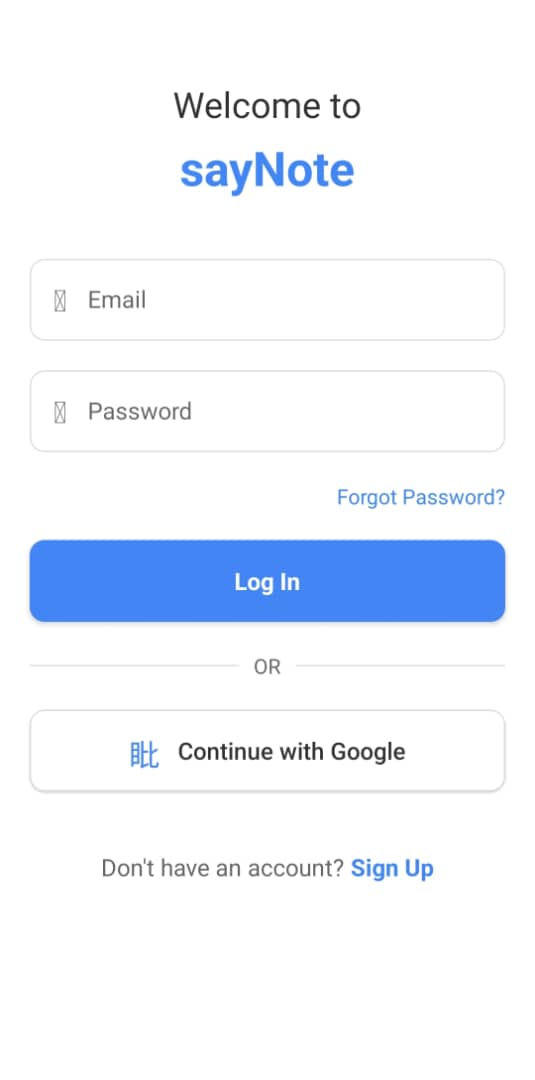
\includegraphics[width=0.4\textwidth]{assets/docs/mobile/login-page.jpeg}
    \hfill
    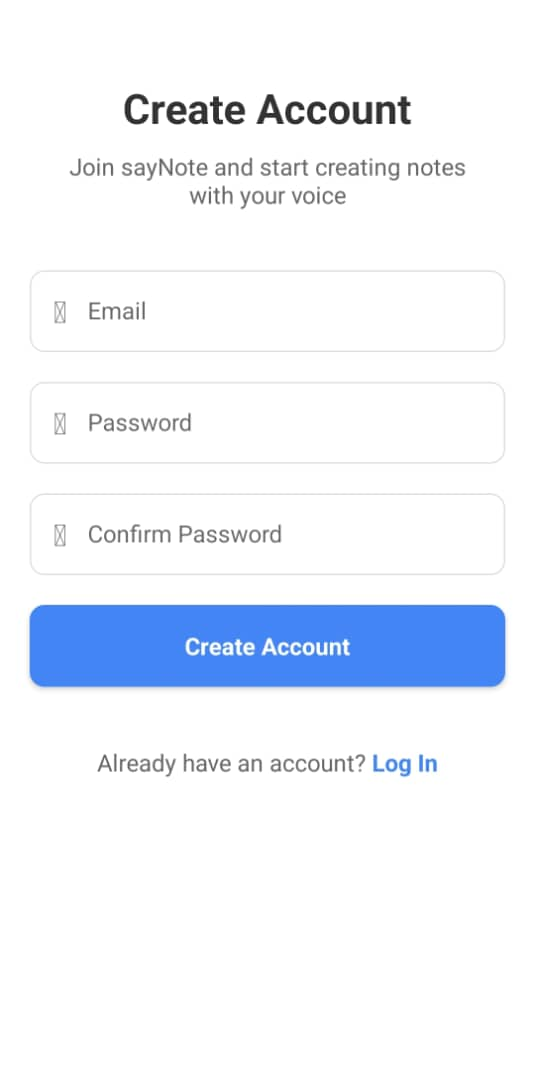
\includegraphics[width=0.4\textwidth]{assets/docs/mobile/create-account-page.jpeg}
    \caption{Écrans de connexion et de création de compte}
    \label{fig:mobile-auth}
\end{figure}

% Explication brève avant chaque figure
\noindent
\textit{La figure suivante illustre un aspect clé de l'architecture ou de l'implémentation technique du système.}
\begin{figure}[H]
    \centering
    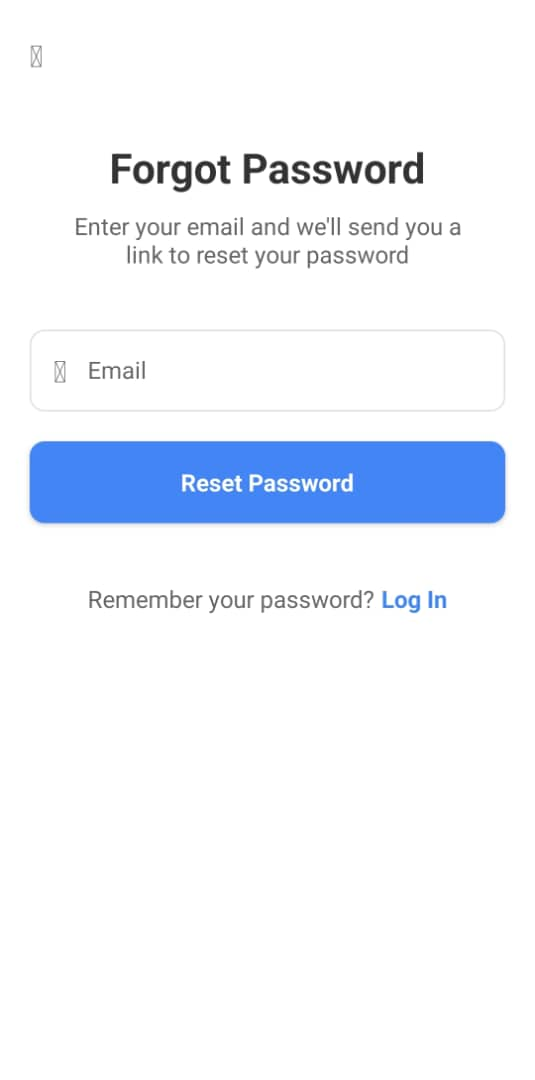
\includegraphics[width=0.4\textwidth]{assets/docs/mobile/forget-password-page.jpeg}
    \caption{Écran de réinitialisation du mot de passe}
    \label{fig:mobile-forgot-password}
\end{figure}

\subsubsection{Navigation et recherche}
% Explication brève avant chaque figure
\noindent
\textit{La figure suivante illustre un aspect clé de l'architecture ou de l'implémentation technique du système.}
\begin{figure}[H]
    \centering
    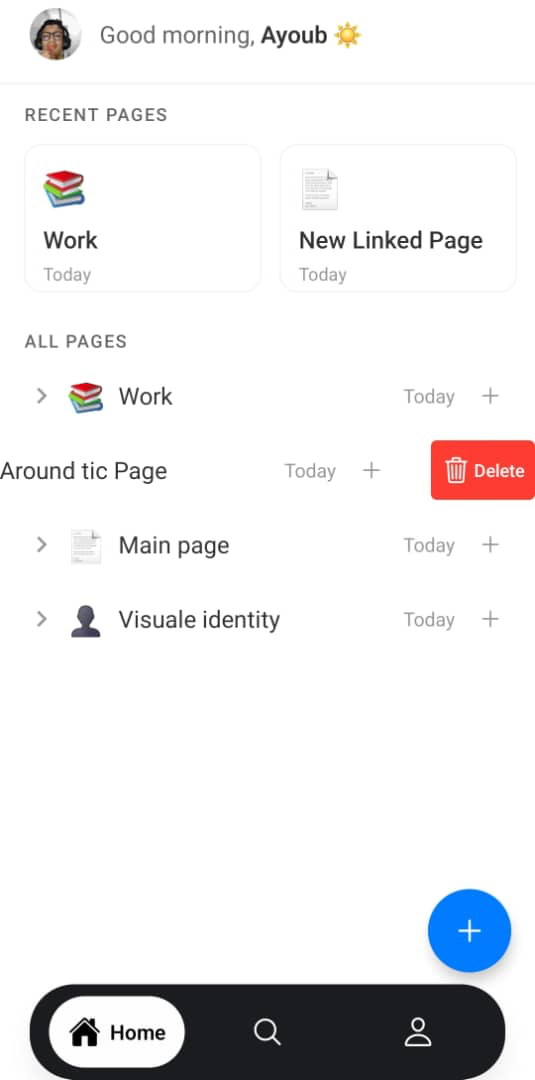
\includegraphics[width=0.4\textwidth]{assets/docs/mobile/home-screen.png}
    \hfill
    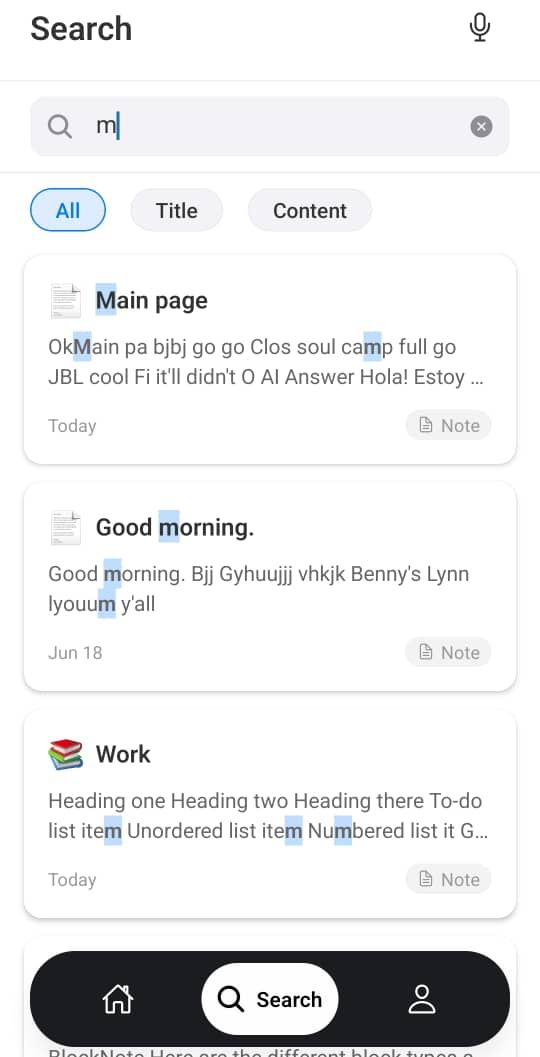
\includegraphics[width=0.4\textwidth]{assets/docs/mobile/search-screeen.png}
    \caption{Écrans d'accueil et de recherche}
    \label{fig:mobile-home-search}
\end{figure}

\subsubsection{Gestion des notes}
% Explication brève avant chaque figure
\noindent
\textit{La figure suivante illustre un aspect clé de l'architecture ou de l'implémentation technique du système.}
\begin{figure}[H]
    \centering
    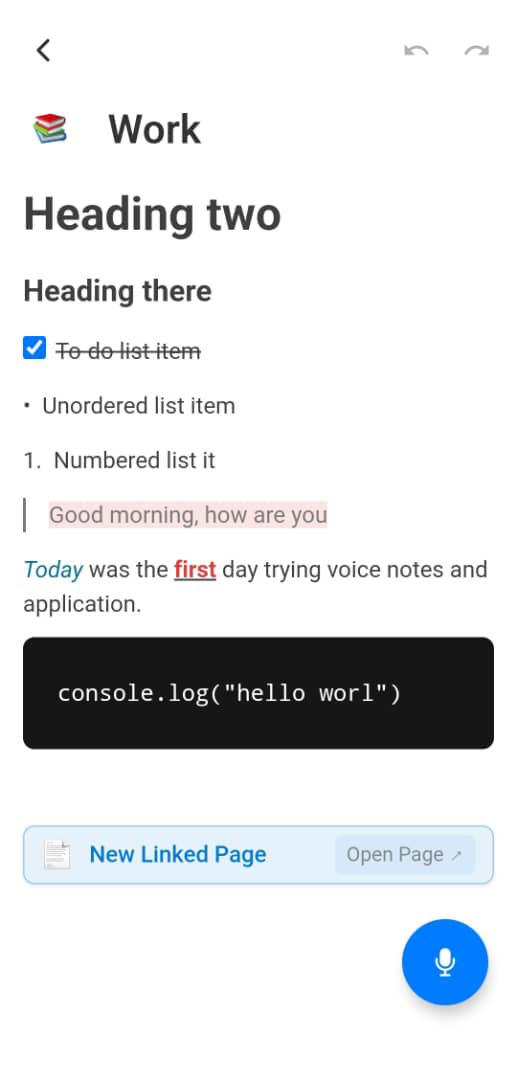
\includegraphics[width=0.4\textwidth]{assets/docs/mobile/note-page.png}
    \hfill
    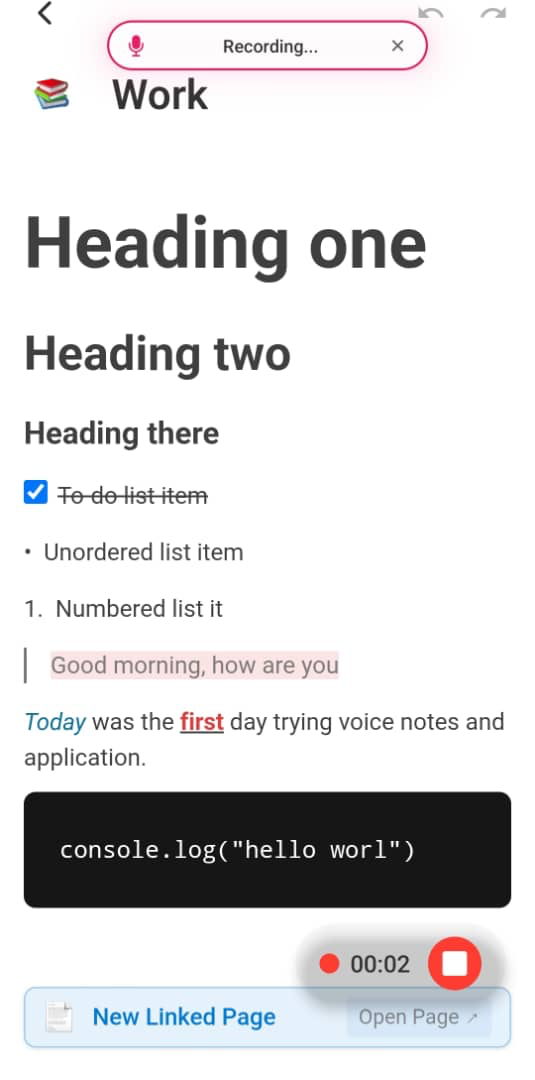
\includegraphics[width=0.4\textwidth]{assets/docs/mobile/note-page-recording.png}
    \caption{Éditeur de notes et enregistrement vocal}
    \label{fig:mobile-editor}
\end{figure}

\subsubsection{Profil utilisateur}
% Explication brève avant chaque figure
\noindent
\textit{La figure suivante illustre  un aspect clé de l'architecture ou de l'implémentation technique du système.}
\begin{figure}[H]
    \centering
    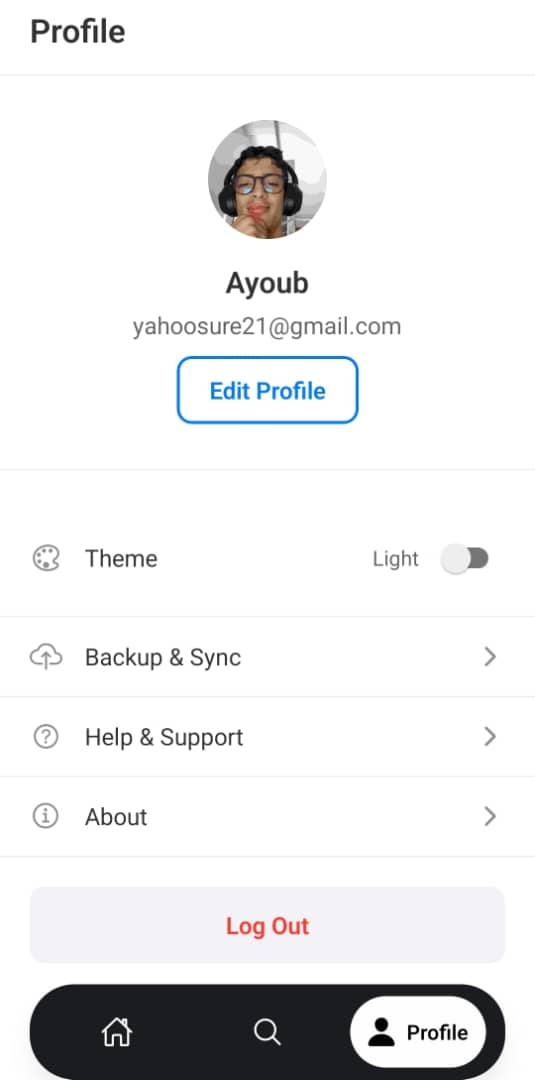
\includegraphics[width=0.4\textwidth]{assets/docs/mobile/profile-screen.png}
    \caption{Écran de profil utilisateur}
    \label{fig:mobile-profile}
\end{figure}

\section{Application web}

\subsection{Technologies et outils utilisés}

\subsubsection{Next.js\resref{res:nextjs}}
Next.js\resref{res:nextjs} est un framework open-source basé sur React, conçu pour le développement d'applications web modernes. Il permet de créer des applications rendues côté serveur (SSR), des sites statiques (SSG), et des applications web monopages (SPA) avec une expérience de développement optimisée.

Pour SayNote, nous avons choisi Next.js pour ses avantages clés:
\begin{itemize}
    \item \textbf{Rendu côté serveur et statique}: Améliore les performances et le SEO.
    \item \textbf{Routing basé sur le système de fichiers}: Simplifie la navigation et l'organisation des pages.
    \item \textbf{Optimisation des images}: Composants d'image intégrés pour un chargement plus rapide.
    \item \textbf{API Routes}: Permet de créer facilement des points de terminaison d'API.
\end{itemize}

\subsubsection{TypeScript}
\begin{wrapfigure}{r}{0.3\textwidth}
    \centering
    
\includegraphics[width=0.25\textwidth]{assets/docs/typescript.png}
\end{wrapfigure}
TypeScript\resref{res:typescript} est un sur-ensemble de JavaScript qui ajoute des types statiques. Il est developpe et maintenu par Microsoft.

Les avantages de TypeScript\resref{res:typescript} que nous avons exploites dans SayNote:
\begin{itemize}
    \item Langage type qui permet de detecter les erreurs lors de la compilation
    \item Compilation en differentes versions ECMAScript a partir de la version 3
    \item Support de la programmation orientee objet
    \item Amelioration de la lisibilite et de la maintenance du code
\end{itemize}

\subsection{Interface de l'Application Web}
Cette section présente les différentes interfaces de l'application web SayNote, illustrant le parcours de l'utilisateur, de l'authentification à la gestion des notes.

\subsubsection{Authentification}
\noindent
\textit{La figure suivante illustre un aspect clé de l'architecture ou de l'implémentation technique du système.}
\begin{figure}[H]
    \centering
    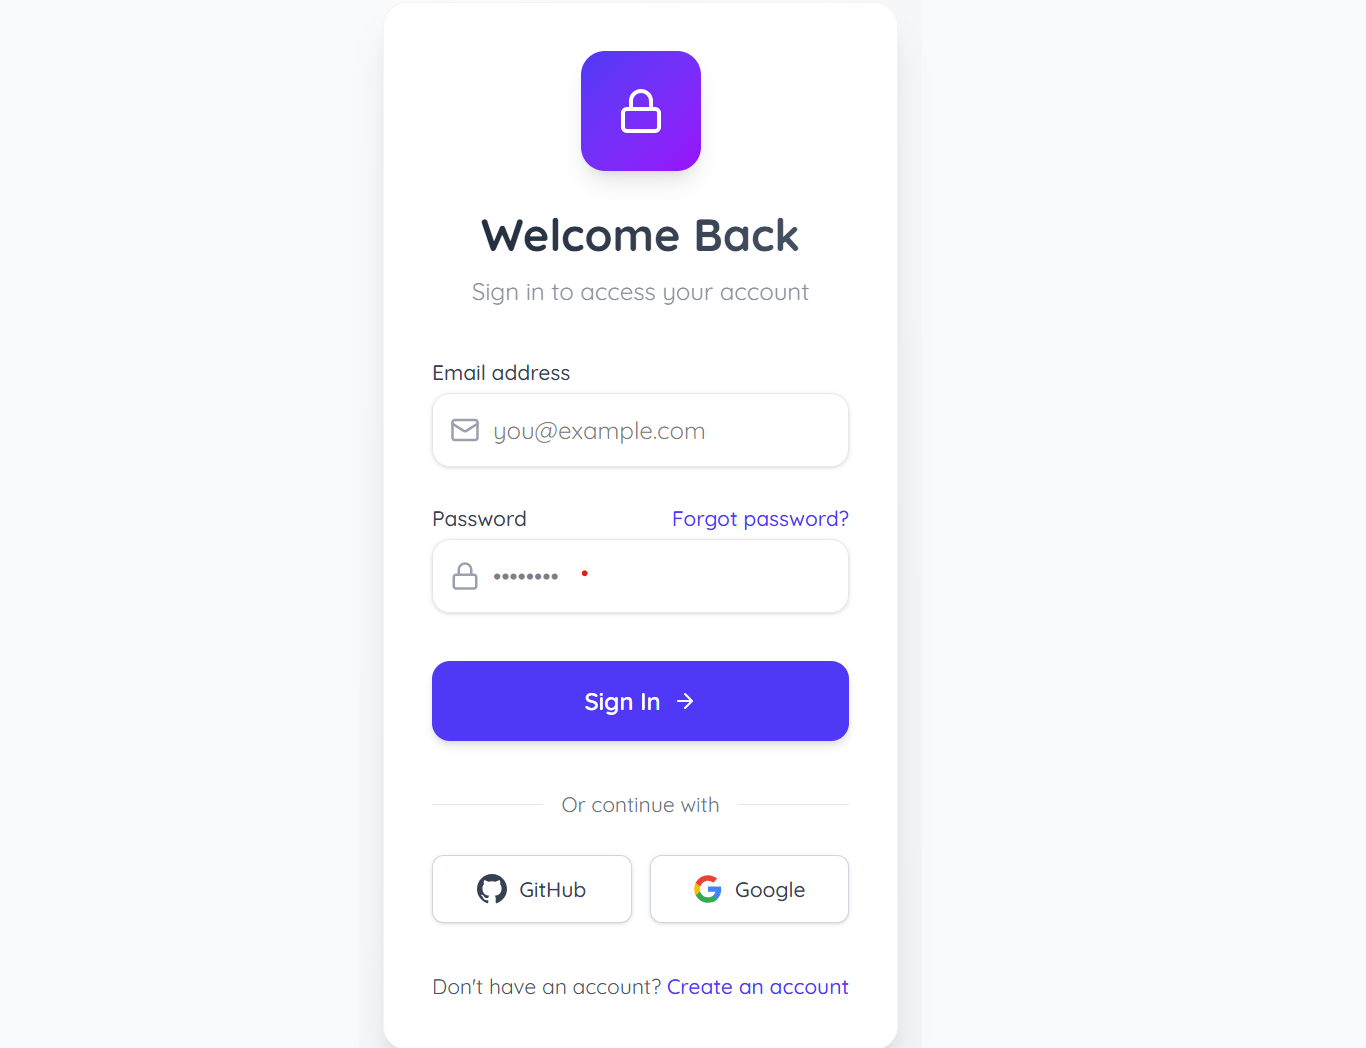
\includegraphics[width=0.45\textwidth]{assets/docs/web/login-page.png}
    \hfill
    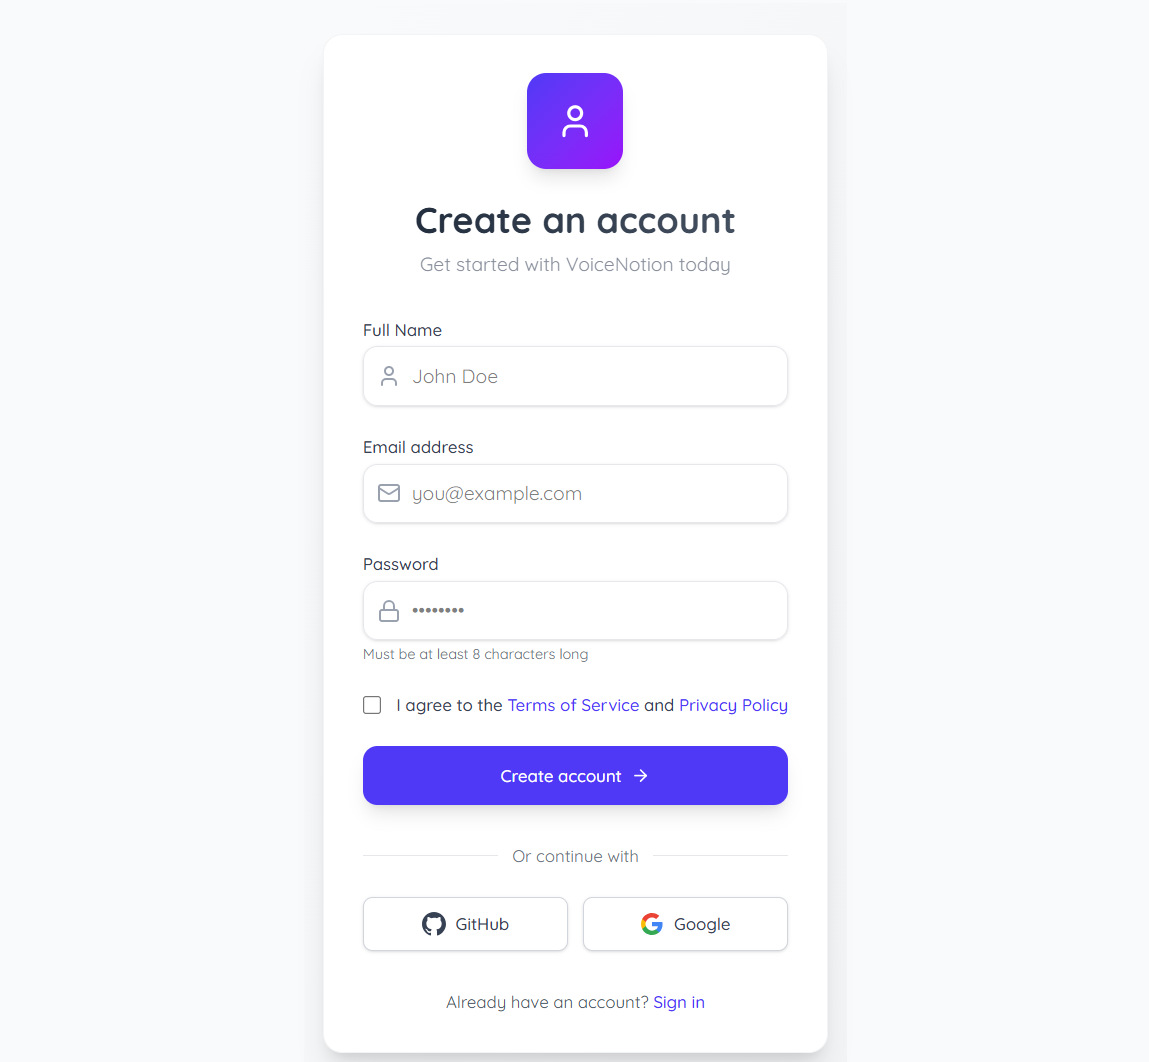
\includegraphics[width=0.45\textwidth]{assets/docs/web/singup.png}
    \caption{Pages de connexion et d'inscription.}
    \label{fig:web-auth}
\end{figure}

\noindent
\textit{La figure suivante illustre un aspect clé de l'architecture ou de l'implémentation technique du système.}
\begin{figure}[H]
    \centering
    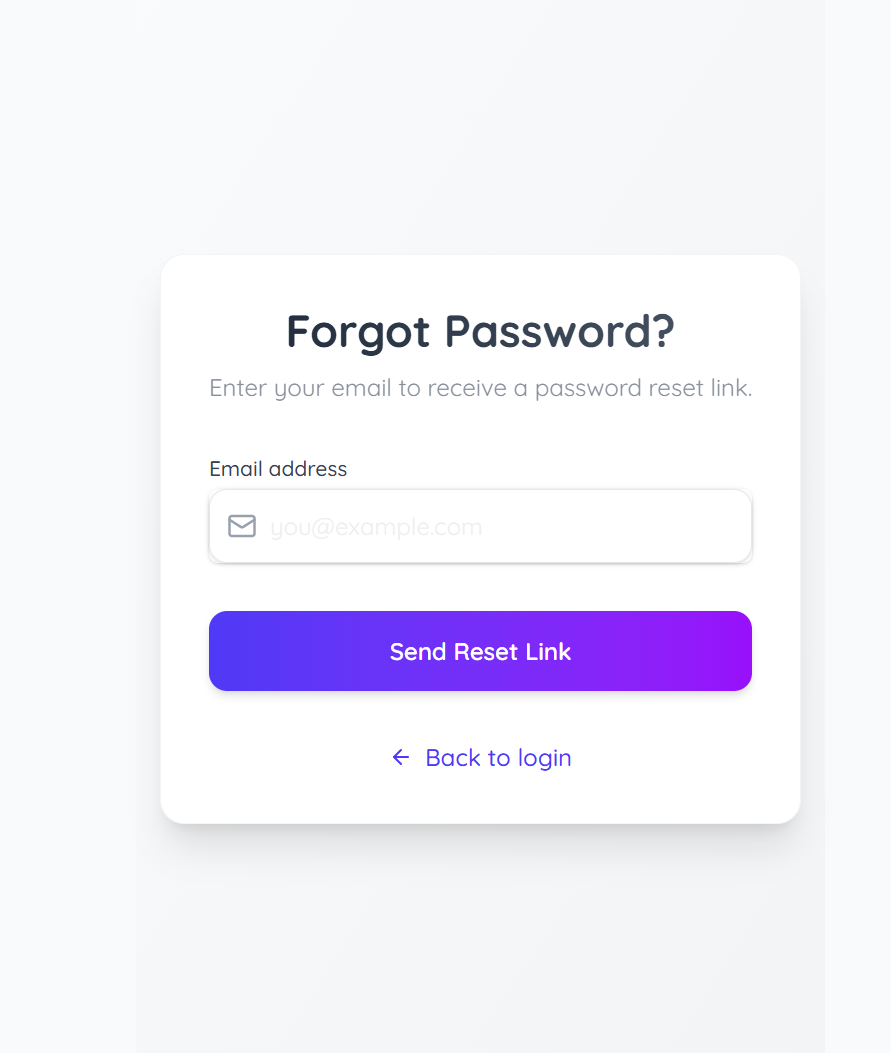
\includegraphics[width=0.45\textwidth]{assets/docs/web/resend-pass.png}
    \hfill
    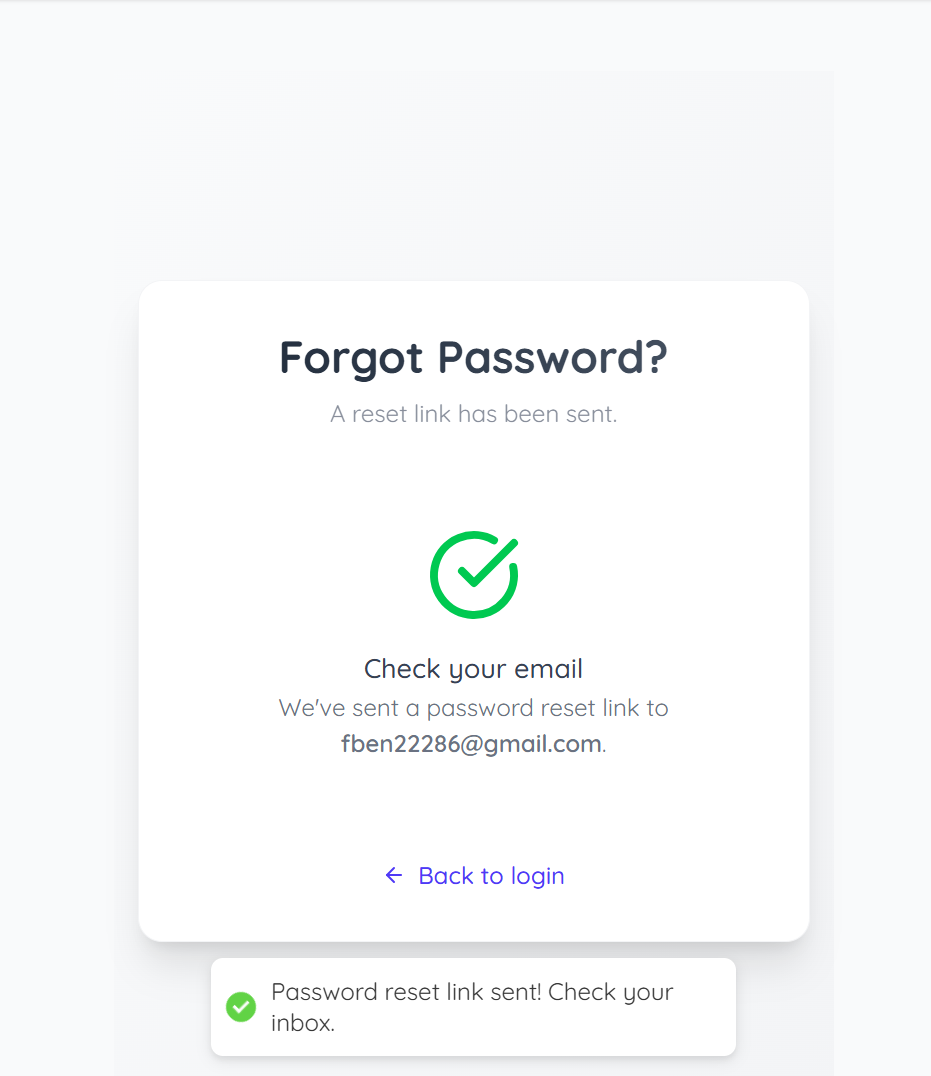
\includegraphics[width=0.45\textwidth]{assets/docs/web/resend-succsus.png}
    \caption{Processus de réinitialisation du mot de passe.}
    \label{fig:web-reset-pass}
\end{figure}

\subsubsection{Tableau de Bord et Paramètres}
\noindent
\textit{La figure suivante illustre un aspect clé de l'architecture ou de l'implémentation technique du système.}
\begin{figure}[H]
    \centering
    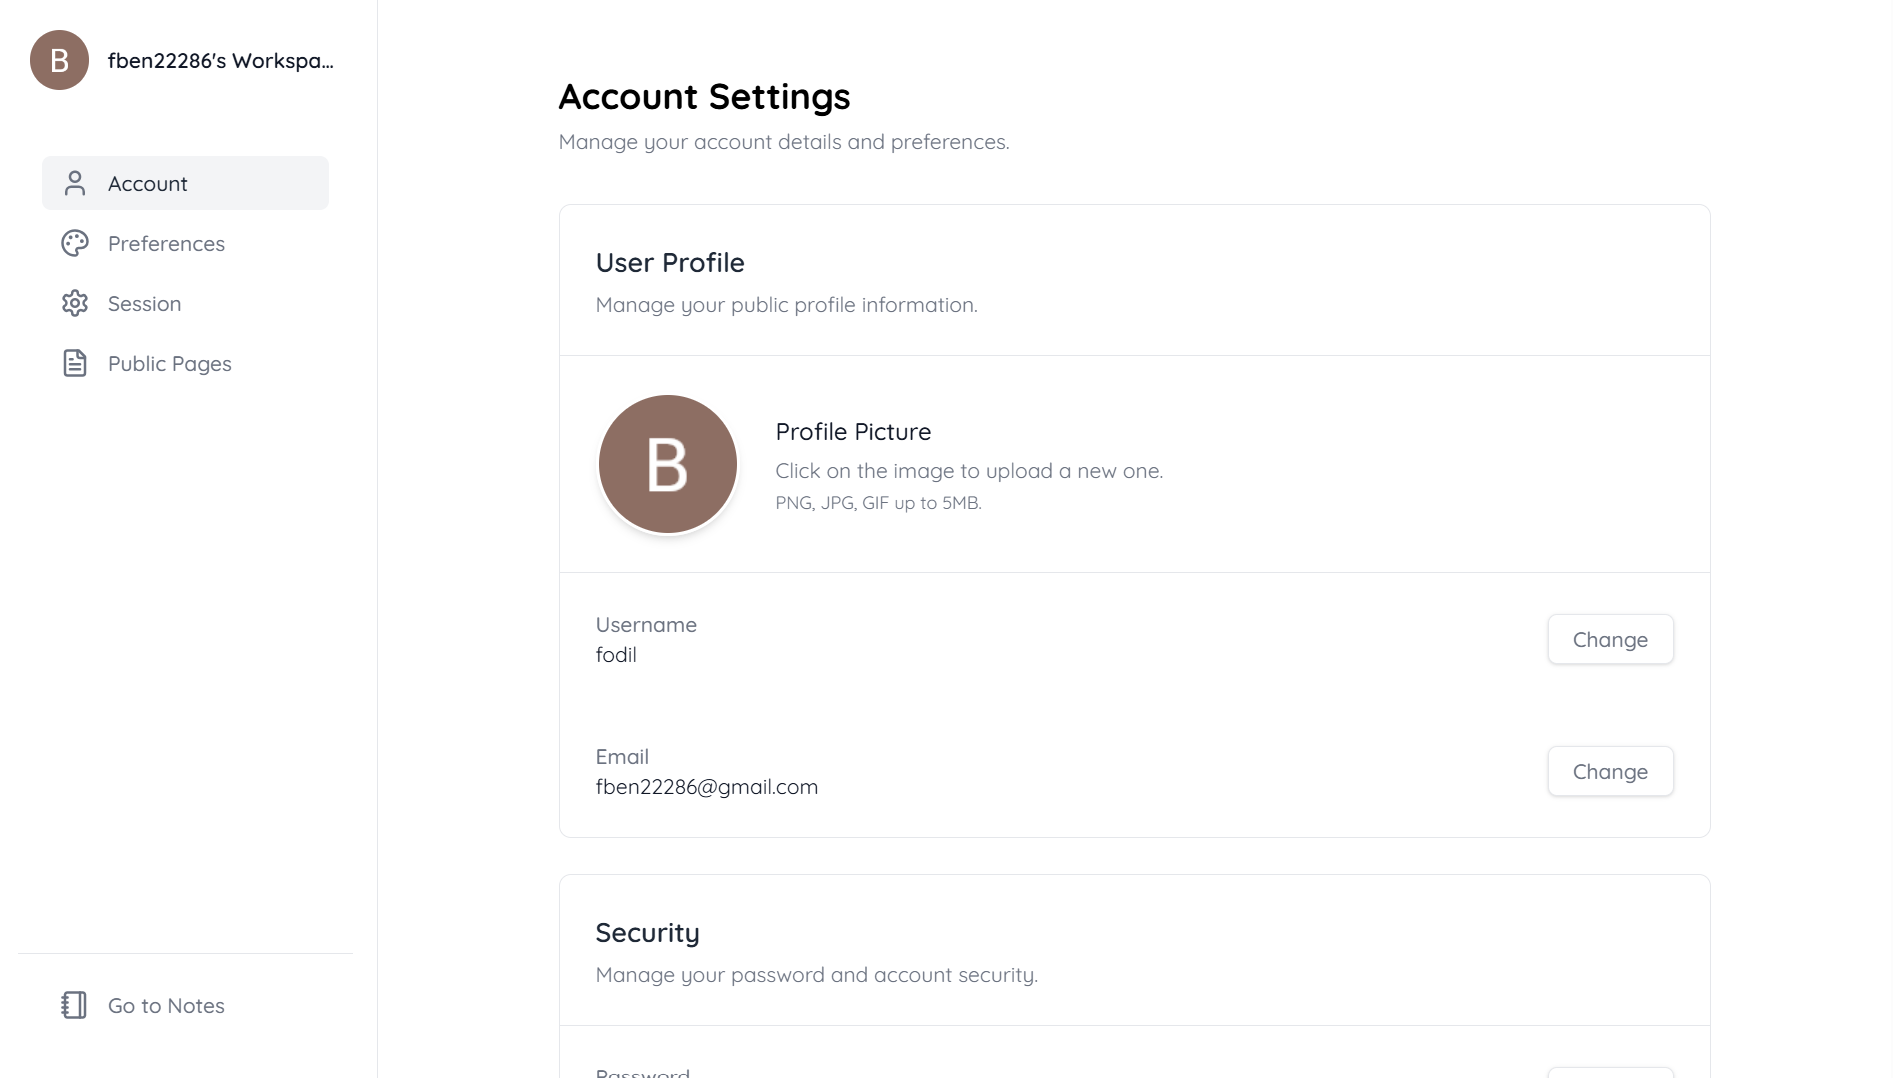
\includegraphics[width=0.8\textwidth]{assets/docs/web/dashboard-page.png}
    \caption{Vue principale du tableau de bord de l'utilisateur.}
    \label{fig:web-dashboard}
\end{figure}

\noindent
\textit{La figure suivante illustre un aspect clé de l'architecture ou de l'implémentation technique du système.}
\begin{figure}[H]
    \centering
    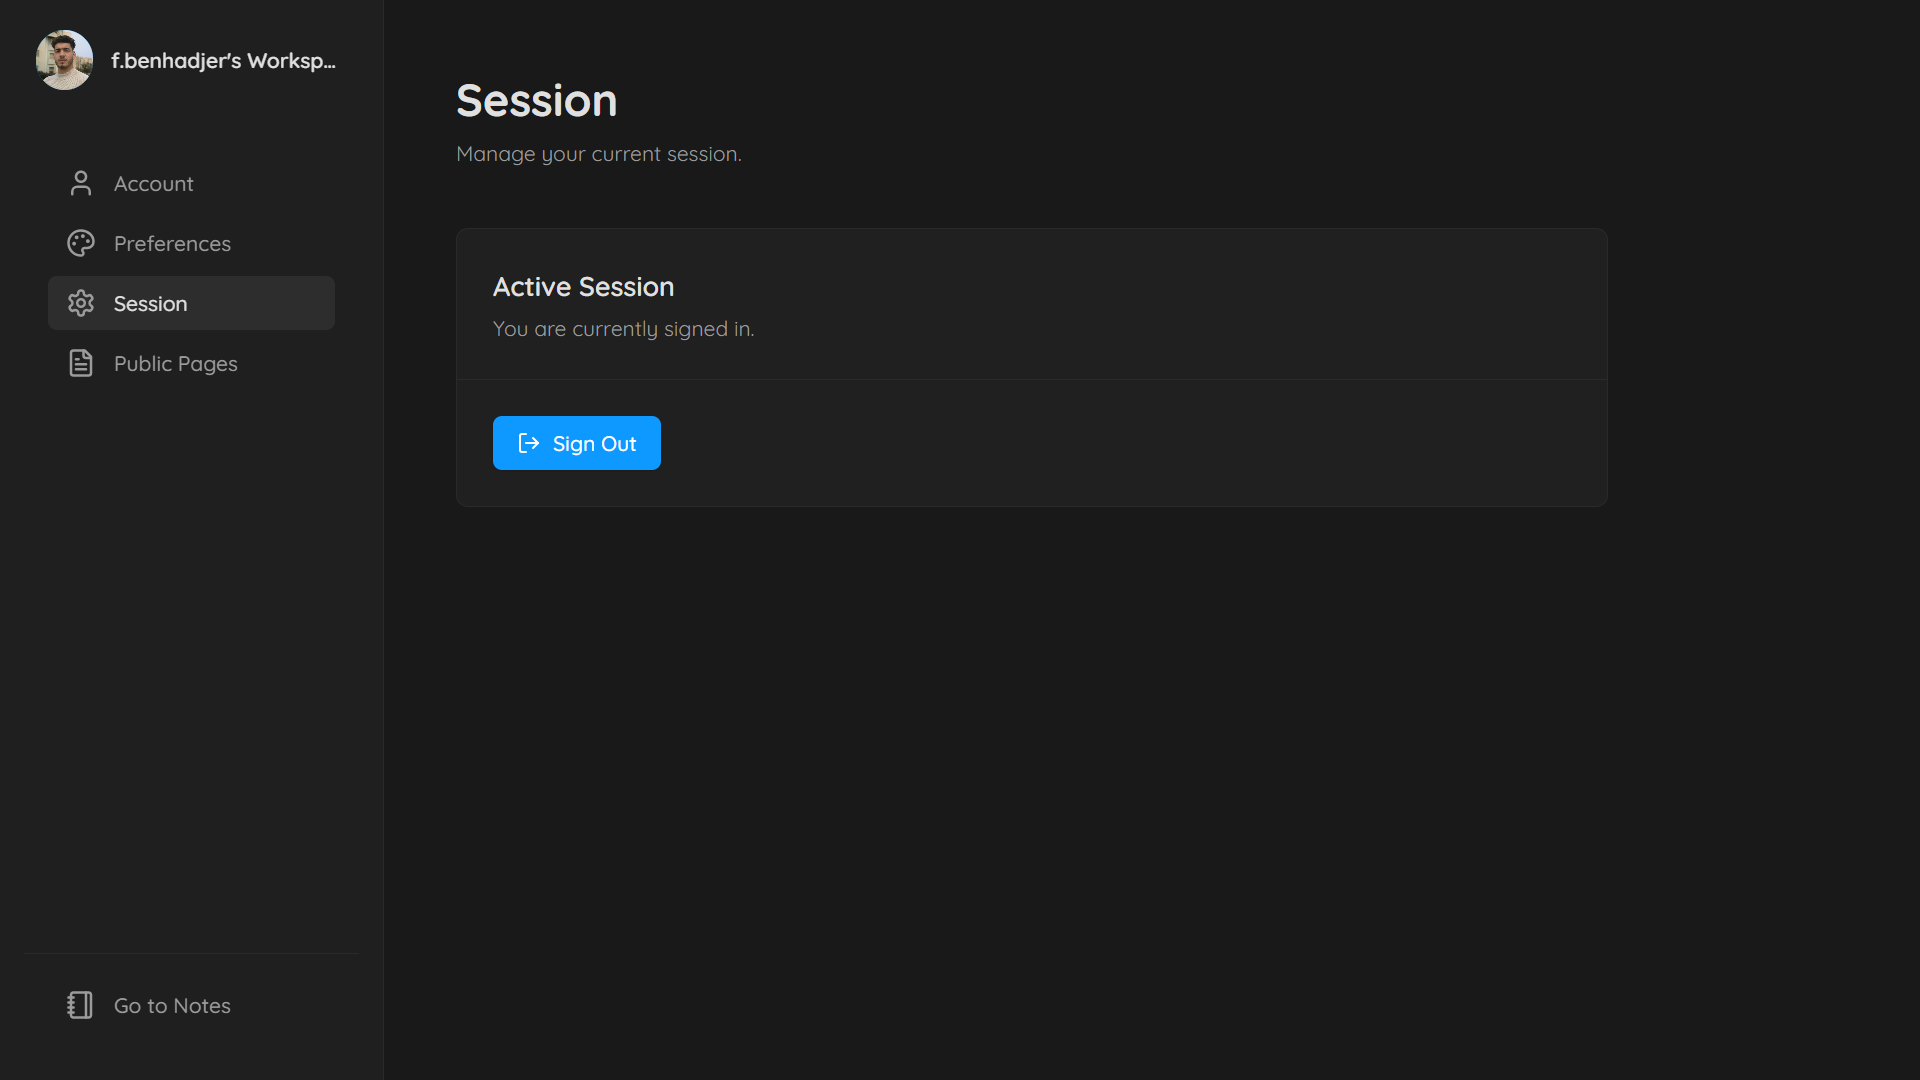
\includegraphics[width=0.45\textwidth]{assets/docs/web/dashboard-appearence-section.png}
    \hfill
    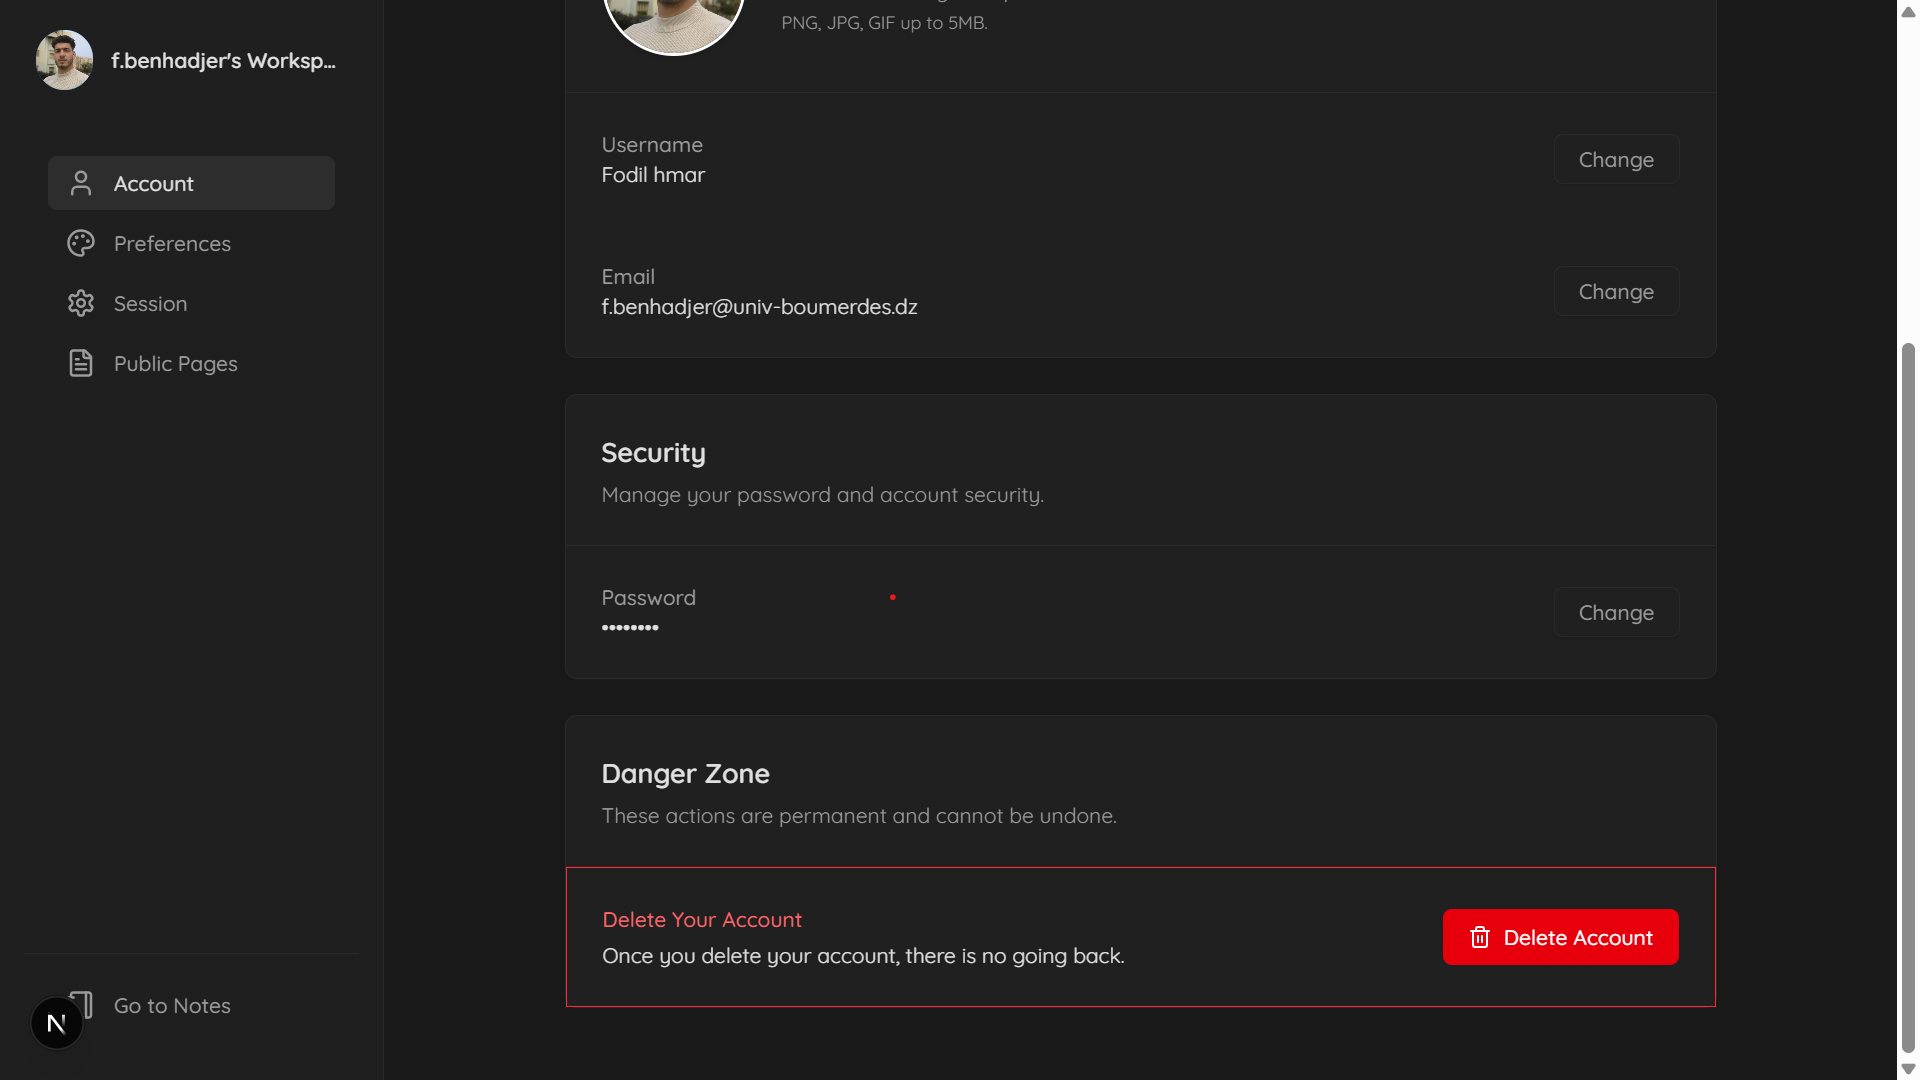
\includegraphics[width=0.45\textwidth]{assets/docs/web/dashboard-page-security-section.png}
    \caption{Sections des paramètres : Apparence et Sécurité.}
    \label{fig:web-settings}
\end{figure}

\subsubsection{Gestion des Notes}
\noindent
\textit{La figure suivante illustre un aspect clé de l'architecture ou de l'implémentation technique du système.}
\begin{figure}[H]
    \centering
    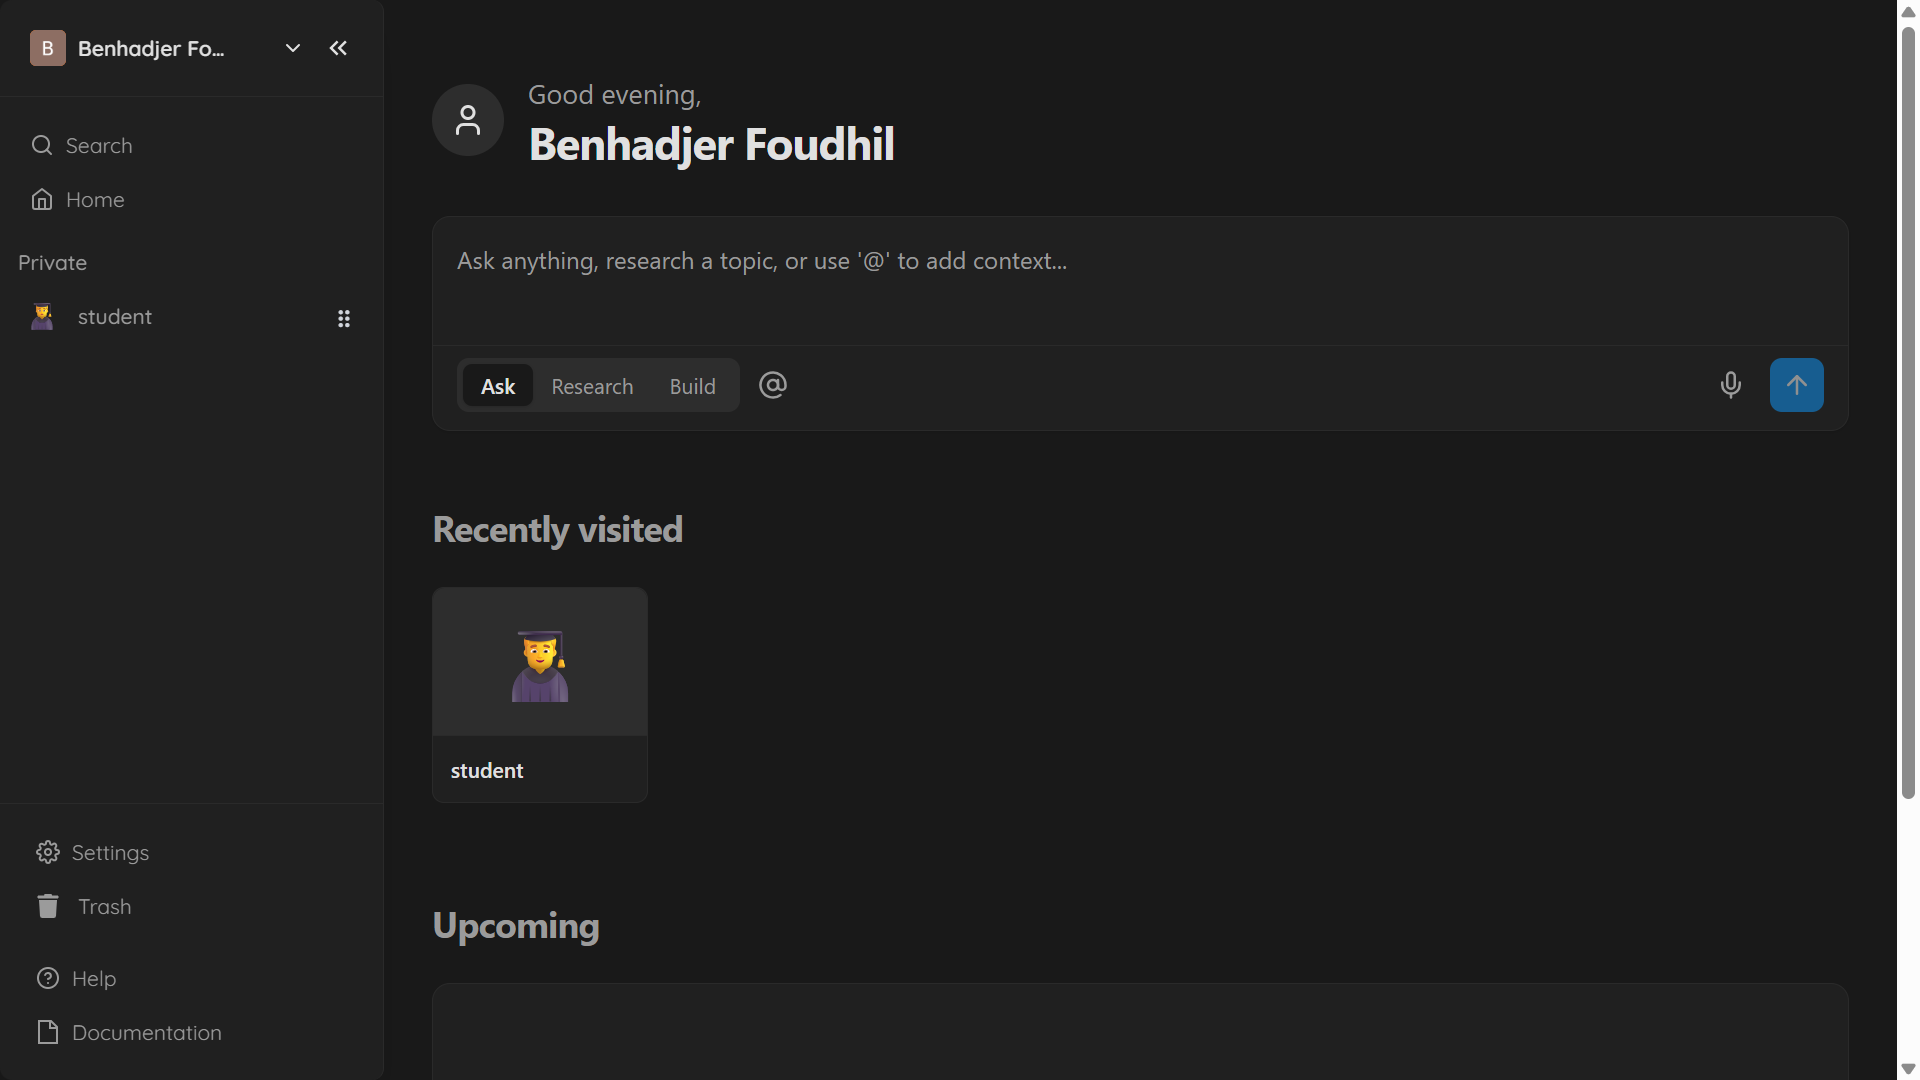
\includegraphics[width=0.45\textwidth]{assets/docs/web/note-homepage.png}
    \hfill
    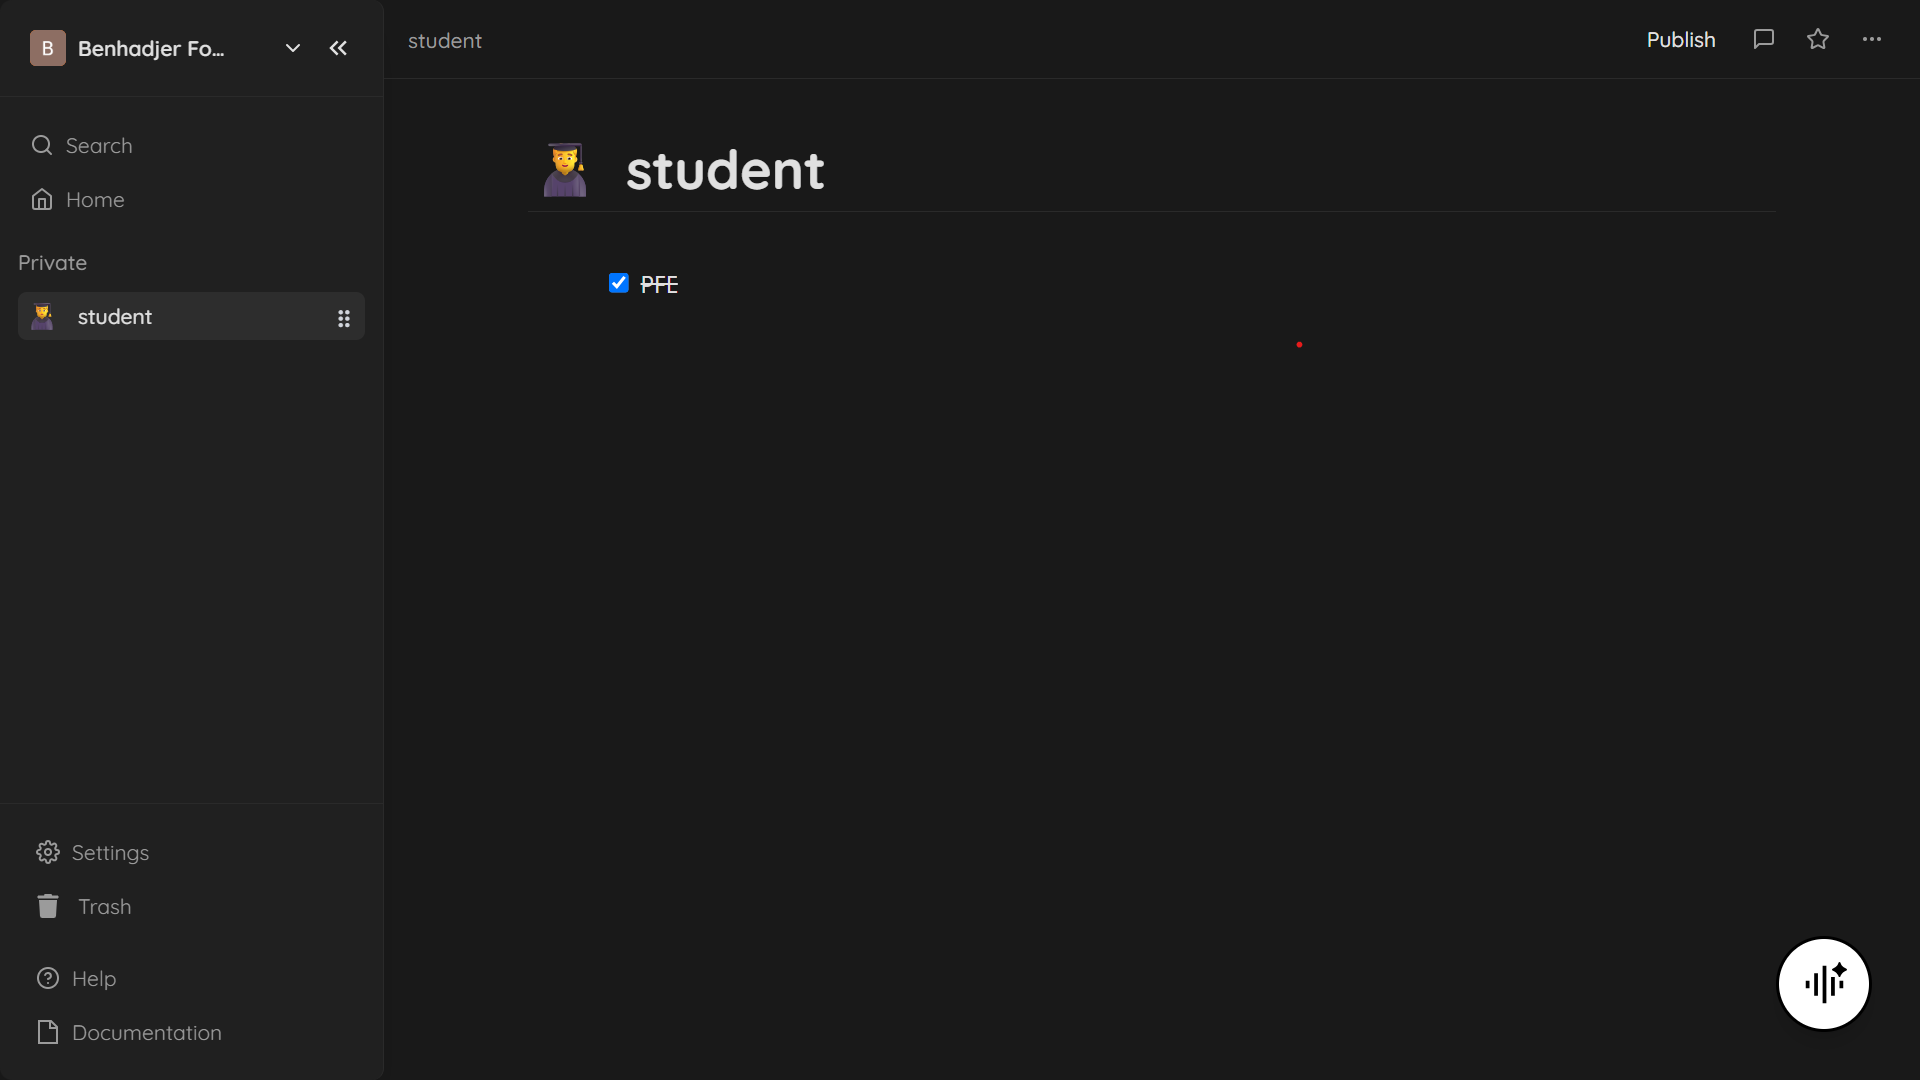
\includegraphics[width=0.45\textwidth]{assets/docs/web/note-page-dark.png}
    \caption{Page d'accueil des notes et éditeur de notes en mode sombre.}
    \label{fig:web-notes}
\end{figure}

\noindent
\textit{La figure suivante illustre un aspect clé de l'architecture ou de l'implémentation technique du système.}
\begin{figure}[H]
    \centering
    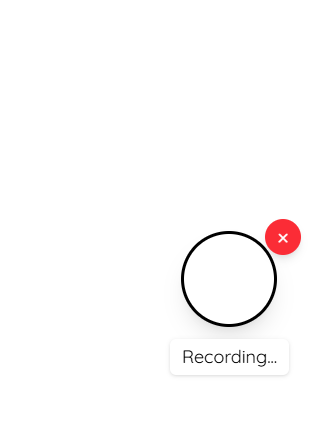
\includegraphics[width=0.45\textwidth]{assets/docs/web/on-record.png}
    \hfill
    
\includegraphics[width=0.45\textwidth]{assets/docs/web/sidebar-search.png}
    \caption{Indicateur d'enregistrement et recherche dans la barre latérale.}
    \label{fig:web-record-search}
\end{figure}

\subsubsection{Publication et Partage}
\noindent
\textit{La figure suivante illustre un aspect clé de l'architecture ou de l'implémentation technique du système.}
\begin{figure}[H]
    \centering
    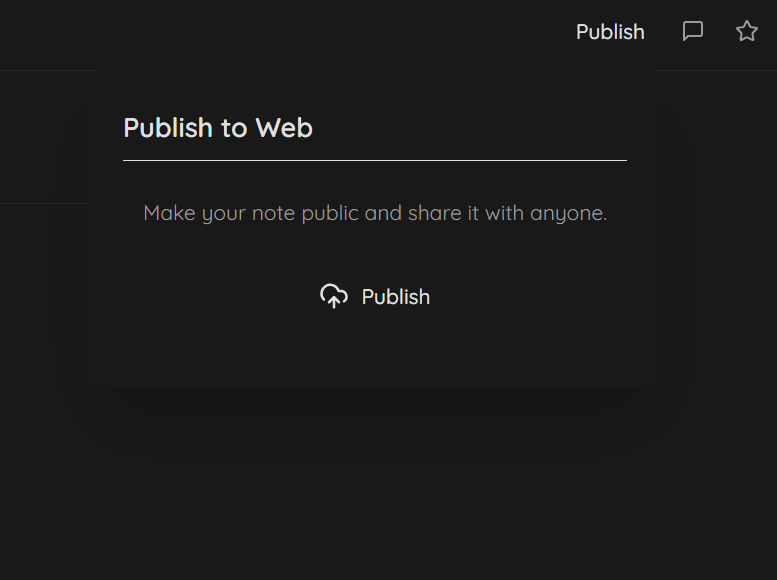
\includegraphics[width=0.45\textwidth]{assets/docs/web/publish-seciton.png}
    \hfill
    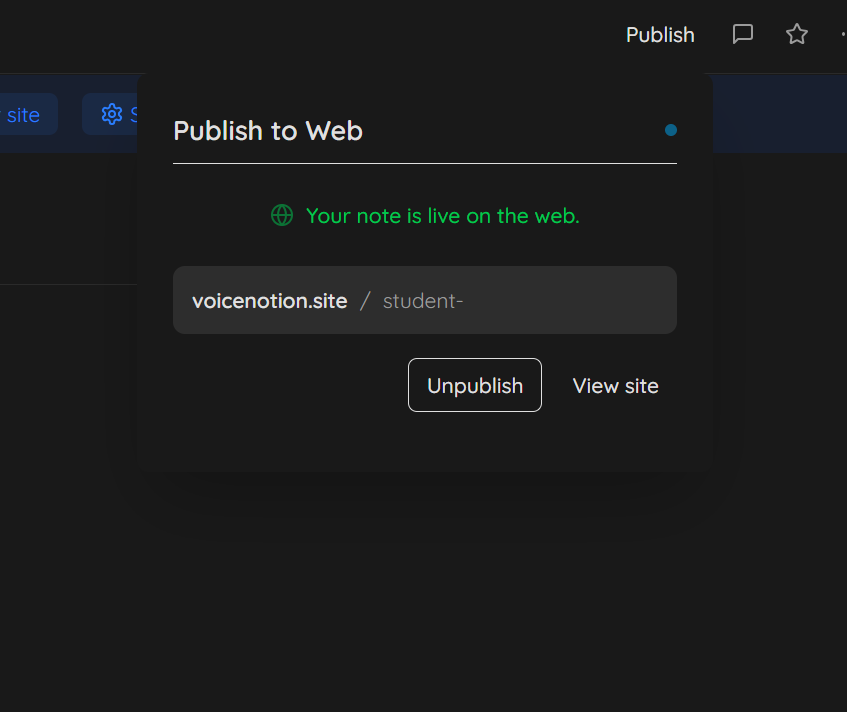
\includegraphics[width=0.45\textwidth]{assets/docs/web/unpublish.png}
    \caption{Options de publication et d'annulation de la publication d'une note.}
    \label{fig:web-publish}
\end{figure}

\noindent
\textit{La figure suivante illustre un aspect clé de l'architecture ou de l'implémentation technique du système.}
\begin{figure}[H]
    \centering
    \includegraphics[width=0.8\textwidth]{assets/docs/web/dashboard-public-page-dark.png}
    \caption{Exemple d'une note publiée accessible publiquement.}
    \label{fig:web-public-note}
\end{figure}




\section{Integration de la reconnaissance vocale}
\subsection{Gemini API}
\begin{minipage}{0.7\textwidth}
L'API Gemini de Google est un modele d'IA multimodal avance qui nous permet d'integrer des capacites de traitement du langage naturel et de comprehension contextuelle dans SayNote. 

Cette API est au coeur de notre fonctionnalite de reconnaissance vocale et nous l'utilisons pour deux fonctions principales:
\begin{itemize}
    \item \textbf{Transcription de la parole en texte (Speech-to-Text)}: Conversion precise de l'audio vocal en texte ecrit
    \item \textbf{Analyse d'intention}: Comprehension et interpretation des commandes vocales pour executer les actions appropriees dans l'application
\end{itemize}

Gemini nous offre plusieurs avantages cles:
\begin{itemize}
    \item \textbf{Comprehension contextuelle}: Capacite a comprendre le contexte des commandes vocales
    \item \textbf{Support multilingue}: Prise en charge de multiples langues pour une utilisation internationale
    \item \textbf{Adaptabilite}: Possibilite d'affiner le modele pour notre cas d'utilisation specifique
    \item \textbf{Integration simple}: API REST facile a integrer dans nos applications web et mobile
\end{itemize}

Grace a Gemini, SayNote peut offrir une experience de dictee vocale naturelle et intuitive, permettant aux utilisateurs de creer et de modifier du contenu a l'aide de commandes vocales complexes.
\end{minipage}%
\hfill
\begin{minipage}{0.25\textwidth}
\centering
\includegraphics[width=0.9\textwidth]{assets/docs/gemini.png}
\end{minipage}

% Explication brève avant chaque figure
\noindent
\textit{La figure suivante illustre le diagramme de l'API Gemini dons SayNote}
\begin{figure}[H]
\centering
\includegraphics[width=0.6\textwidth]{assets/docs/golobal-diagrams/gemini-api-diagram.png}
\caption{Integration de l'API Gemini dans SayNote}
\label{fig:gemini-api}
\end{figure}

\subsection{Flux de traitement des commandes vocales}
Le traitement des commandes vocales dans SayNote suit un flux bien defini:
\begin{enumerate}
    \item Capture de l'audio via le microphone de l'appareil
    \item Conversion de l'audio en texte via l'API Gemini
    \item Analyse de l'intention de la commande (egalement via Gemini)
    \item Execution de l'action correspondante dans l'editeur
    \item Retour visuel et auditif a l'utilisateur
\end{enumerate}

% Explication brève avant chaque figure
\noindent
\textit{La figure suivante illustre le flux de traitement des commandes vocales dans SayNote}
\begin{figure}[H]
\centering
\includegraphics[width=0.6\textwidth]{assets/docs/golobal-diagrams/flux-des-commende-vocal.png}
\caption{Flux de traitement des commandes vocales}
\label{fig:voice-commands-flow}
\end{figure}


\section{Tests et assurance qualite}
\subsection{Strategie de test}
Notre strategie de test pour SayNote comprend plusieurs niveaux:
\begin{itemize}
    \item \textbf{Tests unitaires}: Verification du comportement des composants individuels
    \item \textbf{Tests d'integration}: Validation des interactions entre les differentes parties du systeme
    \item \textbf{Tests end-to-end}: Simulation des parcours utilisateur complets
    \item \textbf{Tests de performance}: Evaluation des temps de reponse et de la consommation de ressources
    \item \textbf{Tests d'accessibilite}: Verification de la conformite aux standards WCAG
\end{itemize}

\subsection{Outils de test}
\begin{itemize}
    \item \textbf{Jest\resref{res:jest}}: Framework de test pour les tests unitaires et d'integration
    \item \textbf{React Testing Library\resref{res:reacttestinglibrary}}: Bibliotheque pour tester les composants React
    \item \textbf{Cypress\resref{res:cypress}}: Outil pour les tests end-to-end de l'application web
    \item \textbf{Detox\resref{res:detox}}: Framework pour les tests end-to-end de l'application mobile
    \item \textbf{Lighthouse\resref{res:lighthouse}}: Outil pour evaluer les performances et l'accessibilite
\end{itemize}

\section{Deploiement et integration continue}
\subsection{Pipeline CI/CD}
Nous avons mis en place un pipeline d'integration continue et de deploiement continu (CI/CD) pour automatiser le processus de build, test et deploiement:

\begin{itemize}
    \item \textbf{GitHub Actions\resref{res:githubactions}}: Automatisation des workflows de CI/CD
    \item \textbf{ESLint et Prettier}: Verification de la qualite du code
    \item \textbf{Tests automatises}: Execution des tests a chaque pull request
    \item \textbf{Preview Deployments}: Deploiement de versions de previsualisation pour chaque branche
\end{itemize}

\subsection{Environnements de deploiement}
\begin{itemize}
    \item \textbf{Developpement}: Environnement local pour les developpeurs
    \item \textbf{Staging}: Environnement de preproduction pour les tests
    \item \textbf{Production}: Environnement final accessible aux utilisateurs
\end{itemize}

\subsection{Plateformes de deploiement}


% --- Deployment ---
\subsubsection{Déploiement Web et Mobile}
Pour assurer une mise en ligne simple et fiable, nous avons opté pour deux solutions de déploiement complémentaires :

\begin{minipage}{0.7\textwidth}
\textbf{Netlify\resref{res:netlify}} : le frontend web (Next.js\resref{res:nextjs}) est automatiquement buildé et publié sur Netlify\resref{res:netlify} à chaque push dans la branche \texttt{main}. Netlify\resref{res:netlify} prend en charge le CDN, le SSL/TLS et le déploiement progressif (rollback en un clic). Des variables d’environnement sécurisées y sont définies pour la connexion à Supabase\resref{res:supabase}.
\end{minipage}%
\hfill
\begin{minipage}{0.25\textwidth}
\centering
\includegraphics[width=0.9\textwidth]{assets/docs/logo_netlify.png}
\end{minipage}

\vspace{0.5cm}

\begin{minipage}{0.7\textwidth}
\textbf{Expo\resref{res:expo}} : l’application mobile React Native\resref{res:reactnative} est distribuée via la plateforme Expo\resref{res:expo}. Grâce à EAS~Build nous générons des APK/IPA signés et, via EAS~Update, nous poussons des OTA updates sans passer par les stores. Les testeurs utilisent Expo\resref{res:expo}~Go pour les versions de pré-production.
\end{minipage}%
\hfill
\begin{minipage}{0.25\textwidth}
\centering
\includegraphics[width=0.9\textwidth]{assets/docs/logo_expo.png}
\end{minipage}

Cette combinaison nous permet un cycle CI/CD unifié : GitHub Actions\resref{res:githubactions} déclenche la génération Netlify\resref{res:netlify} et les builds Expo\resref{res:expo} EAS, garantissant que chaque modification validée est rapidement disponible sur le web et sur mobile.

\section{Securite et protection des donnees}
\subsection{Authentification et autorisation}
La securite de SayNote repose sur plusieurs mecanismes:
\begin{itemize}
    \item \textbf{Authentification multi-facteurs}: Pour une securite renforcee des comptes
    \item \textbf{JWT (JSON Web Tokens)}: Pour la gestion des sessions
    \item \textbf{Controle d'acces base sur les roles}: Pour limiter les actions selon le profil utilisateur
\end{itemize}

\subsection{Protection des donnees}
\begin{itemize}
    \item \textbf{Chiffrement des donnees}: En transit (HTTPS) et au repos
    \item \textbf{Anonymisation}: Des donnees utilisees pour l'analyse et l'amelioration du service
    \item \textbf{Sauvegarde reguliere}: Pour prevenir la perte de donnees
\end{itemize}

\subsection{Conformite RGPD}
SayNote est concu dans le respect du Reglement General sur la Protection des Donnees:
\begin{itemize}
    \item \textbf{Consentement explicite}: Pour la collecte et l'utilisation des donnees
    \item \textbf{Droit a l'oubli}: Possibilite de supprimer toutes les donnees utilisateur
    \item \textbf{Portabilite des donnees}: Export des notes dans des formats standards
\end{itemize}

\section{Defis techniques et solutions}
\subsection{Defis rencontres}
Durant le developpement de SayNote, nous avons rencontre plusieurs defis techniques:
\begin{itemize}
    \item \textbf{Precision de la reconnaissance vocale}: Particulierement dans des environnements bruyants
    \item \textbf{Synchronisation en temps reel}: Entre les differents appareils d'un utilisateur
    \item \textbf{Performance de l'editeur}: Avec des documents volumineux
    \item \textbf{Fonctionnement hors ligne}: Gestion des conflits lors de la reconnexion
\end{itemize}

\subsection{Solutions implementees}
\begin{itemize}
    \item \textbf{Filtrage audio}: Algorithmes de reduction du bruit pour ameliorer la reconnaissance vocale
    \item \textbf{Systeme de replication}: Base sur CRDT (Yjs\resref{res:crdt}) pour la synchronisation
    \item \textbf{Virtualisation}: Rendu optimise des longs documents pour maintenir la performance
    \item \textbf{Queue de synchronisation}: Pour gerer les modifications hors ligne et les synchroniser lors de la reconnexion
\end{itemize}



\section*{Conclusion}
\addcontentsline{toc}{section}{Conclusion}
L'implémentation de SayNote a nécessité l'intégration de nombreuses technologies modernes et la résolution de défis techniques complexes. L'architecture choisie nous a permis de créer une application performante, sécurisée et évolutive, disponible sur le web et sur mobile. La combinaison de React, Next.js\resref{res:nextjs}, React Native\resref{res:reactnative} et Supabase\resref{res:supabase} nous a fourni une base solide, tandis que l'intégration de l'API Gemini a rendu possible la fonctionnalité centrale de reconnaissance vocale.

En résumé, ce chapitre a détaillé l'ensemble des choix techniques, des architectures et des solutions mises en œuvre pour concrétiser SayNote. L'intégration harmonieuse des différentes technologies et la résolution des défis techniques témoignent de la robustesse et de la modernité de l'application. Ces fondations solides ouvrent la voie à de futures évolutions, comme l'amélioration continue de la précision de la reconnaissance vocale, l'ajout de nouvelles fonctionnalités collaboratives, et l'optimisation des performances sur tous les appareils.

\chapter{IDENTITE VISUELLE}
% \chapter{CHAPITRE 4 : SAYNOTE – VISUAL IDENTITY}

% --- Introduction non numérotée ---
\begin{center}
\textbf{\large Introduction du Chapitre}
\end{center}

\noindent
Ce chapitre présente la démarche de création et les choix fondamentaux de l'identité visuelle pour SayNote. Il met en avant l'importance du branding, des couleurs, de la typographie et des supports graphiques pour garantir une expérience utilisateur cohérente et mémorable, tout en valorisant la marque sur tous les supports.

\section{Introduction}
Dans ce chapitre nous parlerons de notre identité visuelle. (Couleurs, typographie, charte graphique, design commercial, ...).

\section{Logo}
\subsection{Name selection}
\begin{tcolorbox}[colback=SayNoteLightGray!10!white, title=Origine du nom]
Le nom \textbf{Saynote} a été soigneusement choisi pour refléter la mission principale de l'application : permettre aux utilisateurs de capturer instantanément leurs idées à l’aide de leur voix. Simple, intuitif et signifiant, « Saynote » incarne l’intersection entre la parole et la productivité. C’est plus qu’un nom, c’est une expérience en un mot.
\end{tcolorbox}

\textbf{Décomposition du nom~:} \textit{Saynote = Say + Note}
\begin{itemize}
    \item \textbf{Say}~: Interaction vocale, rapidité, facilité, communication naturelle.
    \item \textbf{Note}~: Capture structurée d’idées, rappels, tâches.
\end{itemize}

\noindent
Ensemble, Saynote devient une commande, un comportement et une marque : il suffit de «~dire sa note~».

\textbf{Message et sens~:}
\begin{itemize}
    \item Vous n’avez plus besoin de taper. Il suffit de parler : votre voix devient une note.
    \item Un seul geste, un seul outil, un seul résultat. Dites-le, sauvegardez-le : terminé.
\end{itemize}

\subsection{Logo selection}
Le logo SayNote combine une onde vocale stylisée et la forme d’un bloc-notes, symbolisant la fusion entre la saisie vocale et l’organisation des idées. Le dégradé bleu doux évoque le calme et la clarté, tandis que les coins arrondis et le détail du coin replié ajoutent une touche conviviale et moderne.

\begin{itemize}
    \item \textbf{Simplicité} : Formes minimales, reconnaissance immédiate.
    \item \textbf{Clarté} : Chaque élément a un but précis : outil de prise de notes avec intégration vocale.
    \item \textbf{Esthétique propre} : Courbes douces, contours nets, adaptable sur fond clair ou sombre.
    \item \textbf{Symbolisme} : Rapidité, simplicité, innovation, focus.
    \item \textbf{Adaptabilité} : Le logo reste lisible et impactant à toutes tailles.
\end{itemize}

\subsection{Design methodology}
% Explication brève avant chaque figure
\noindent
\textit{La figure suivante illustre un élément clé de l'identité visuelle ou de la communication de la marque.}
\begin{figure}[H]
    \centering
    \includegraphics[width=0.25\textwidth]{docs/visual-indentity/pictures/logo.png}
    \caption{Logo principal SayNote. \newline\textit{Ce logo fusionne la notion de voix et de prise de notes, représentant la mission centrale de l'application.}}
\end{figure}

% Explication brève avant chaque figure
\noindent
\textit{La figure suivante illustre un élément clé de l'identité visuelle ou de la communication de la marque.}
\begin{figure}[H]
    \centering
    \includegraphics[width=0.7\textwidth]{docs/visual-indentity/pictures/logo-varaition-blue.jpg}
    \caption{Variante bleu du logo. \newline\textit{Cette version met en avant la modernité et la fraîcheur de la marque.}}
\end{figure}

% Explication brève avant chaque figure
\noindent
\textit{La figure suivante illustre un élément clé de l'identité visuelle ou de la communication de la marque.}
\begin{figure}[H]
    \centering
    \includegraphics[width=0.7\textwidth]{docs/visual-indentity/pictures/logo-variation-black-and-white.jpg}
    \caption{Logo noir et blanc. \newline\textit{Cette variante assure la lisibilité et l'adaptabilité sur différents supports.}}
\end{figure}

\section{Typographie}
Les polices sans empattement constituent un élément clé de l’identité visuelle de SayNote. Ce choix traduit notre volonté d’offrir une esthétique moderne, épurée et conviviale.

\textbf{a) Police pour les titres}
La police principale d’affichage se distingue par un design géométrique et affirmé, apportant clarté et structure aux titres et messages clés. Ses lignes minimalistes et proportions équilibrées la rendent idéale pour les titres, slogans et zones nécessitant un fort impact visuel.

\textbf{b) Police de contenu}
La police de texte principale est chaleureuse, accueillante et hautement lisible sur tous supports. Ses formes arrondies et son flux harmonieux insufflent une sensation de calme et de proximité à la marque. Elle garantit une excellente lisibilité, même en petite taille, et s’adapte parfaitement aux textes courants, éléments d’interface et contenus étendus.

Ensemble, ces deux polices créent un équilibre harmonieux entre structure et douceur, parfaitement aligné avec l’identité vocale, claire et joyeuse de SayNote.

% Explication brève avant chaque figure
\noindent
\textit{La figure suivante illustre un élément clé de l'identité visuelle ou de la communication de la marque.}
\begin{figure}[H]
    \centering
    \includegraphics[width=0.7\textwidth]{docs/visual-indentity/pictures/primary-font.png}
    \caption{Police principale SayNote : structure et impact pour les titres. \newline\textit{Cette police renforce la clarté et la hiérarchie visuelle des contenus.}}
\end{figure}
% Explication brève avant chaque figure
\noindent
\textit{La figure suivante illustre un élément clé de l'identité visuelle ou de la communication de la marque.}
\begin{figure}[H]
    \centering
    \includegraphics[width=0.7\textwidth]{docs/visual-indentity/pictures/secondery-font.png}
    \caption{Police de contenu SayNote : lisibilité, chaleur et modernité. \newline\textit{Ce choix garantit une lecture agréable et une identité chaleureuse.}}
\end{figure}

\textbf{Titres~:}
Police sans-serif, géométrique, épaisse, pour la clarté et la structure.

\textbf{Corps de texte~:}
Police sans-serif, arrondie et chaleureuse, pour la lisibilité et l’accessibilité.

L’association des deux polices crée un équilibre entre structure et douceur, fidèle à l’esprit SayNote.

\section{Palette de couleurs}
\subsection{Bleu principal — \#4385F6}
Ce bleu vibrant représente la clarté, la confiance et un design intelligent. Il évoque le calme du ciel et la fiabilité des outils numériques modernes. Élément central de l’identité SayNote, il symbolise la concentration, la productivité et la confiance, en parfaite adéquation avec notre objectif d’une expérience vocale sans distraction.

\subsection{Bleus profonds — \#1E6DE0, \#0043A5, \#002E72}
Ces nuances plus sombres complètent la couleur principale en ajoutant profondeur et contraste. Elles reflètent la structure et la clarté de l’interface SayNote, renforçant la stabilité, la précision et une sensation de contrôle calme.

\subsection{Accent clair — \#CFE3FF}
Cet accent pastel doux apporte une touche de légèreté et de joie à l’ensemble de la marque. Il confère une qualité rafraîchissante et aérée à l’interface tout en améliorant la hiérarchie visuelle et l’accessibilité. Il soutient notre ton de clarté et de sérénité, équilibrant les bleus plus soutenus.

% Explication brève avant chaque figure
\noindent
\textit{La figure suivante illustre un élément clé de l'identité visuelle ou de la communication de la marque.}
\begin{figure}[H]
    \centering
    \includegraphics[width=0.6\textwidth]{docs/visual-indentity/pictures/color-palette.png}
    \caption{Palette de couleurs SayNote : harmonie, clarté et confiance.}
\end{figure}

En combinant ces couleurs, SayNote propose un système visuel harmonieux et émotionnellement aligné, reflétant nos valeurs fondamentales : clarté, confiance, inclusivité et productivité sereine.

\section{Stationery \& Visual Imagination}
\subsection{Design}
La papeterie SayNote comprend une gamme complète de supports imprimés, conçus pour refléter l'identité visuelle de la marque et renforcer la cohérence graphique dans toutes les communications professionnelles.

\subsubsection*{Carte de visite}
La carte de visite SayNote reprend les codes graphiques de la marque : couleurs, typographie et logo. Elle offre une présentation professionnelle et mémorable lors des échanges.
% Explication brève avant chaque figure
\noindent
\textit{La figure suivante illustre un élément clé de l'identité visuelle ou de la communication de la marque.}
\begin{figure}[H]
    \centering
    \includegraphics[width=0.5\textwidth]{docs/visual-indentity/pictures/card.jpg}
    \caption{Carte de visite SayNote : design épuré et impactant. \newline\textit{Un support professionnel qui véhicule l'identité de la marque.}}
\end{figure}

\subsection{Poster}
\subsubsection*{a) Concept du design}
Le concept du poster repose sur l'attraction visuelle, l'expression de l'identité de la marque et la mise en avant des fonctionnalités clés de SayNote. La composition soigneusement pensée allie des images frappantes, des couleurs vibrantes de la marque et un texte concis et percutant pour assurer lisibilité et impact. Les posters finaux sont conçus au format A3.

\subsubsection*{b) Versions}
Deux versions de posters ont été réalisées pour répondre à différents usages et publics. La première met l’accent sur la productivité vocale de SayNote, tandis que la seconde valorise la clarté et la fluidité apportées par l’IA et le design. Les deux affiches conservent une cohérence visuelle tout en ciblant des besoins et contextes variés.

\subsubsection*{c) Développement du contenu}
Le contenu a été élaboré pour délivrer un message convaincant : titres accrocheurs, valeurs essentielles et un appel à l’action clair (téléchargement de l’application ou visite du site). Les visuels et le texte reflètent le ton de la marque : calme, clarté, soutien et modernité.

% Explication brève avant chaque figure
\noindent
\textit{La figure suivante illustre un élément clé de l'identité visuelle ou de la communication de la marque.}
\begin{figure}[H]
    \centering
    \includegraphics[width=0.8\textwidth]{docs/visual-indentity/pictures/poster2.jpg}
    \caption{Poster SayNote : version "Productivité Vocale" – met en avant la rapidité et la simplicité de la prise de notes par la voix. \newline\textit{Ce poster valorise l'usage vocal et la modernité de l'application.}}
\end{figure}
% Explication brève avant chaque figure
\noindent
\textit{La figure suivante illustre un élément clé de l'identité visuelle ou de la communication de la marque.}
\begin{figure}[H]
    \centering
    \includegraphics[width=0.8\textwidth]{docs/visual-indentity/pictures/poster.jpg}
    \caption{Poster SayNote : version "Clarté et Innovation" – valorise la fluidité, la technologie et le design moderne de l’application.}
\end{figure}

\subsection{Banner}
\subsubsection*{a) Concept du design}
La bannière SayNote est conçue pour renforcer la présence visuelle de la marque lors d’événements ou dans des espaces digitaux. Elle s’appuie sur une composition graphique forte, des couleurs distinctives et des éléments identitaires pour attirer l’attention et transmettre les valeurs du projet.

\subsubsection*{b) Développement du contenu}
Les messages mis en avant sur la bannière sont pensés pour promouvoir la crédibilité, la modernité et la cohérence de la marque, tout en assurant une lisibilité optimale à distance. Les éléments graphiques sont harmonisés avec l’ensemble de la papeterie et des supports visuels.

\subsubsection*{c) Éléments visuels}
% Explication brève avant chaque figure
\noindent
\textit{La figure suivante illustre un élément clé de l'identité visuelle ou de la communication de la marque.}
\begin{figure}[H]
    \centering
    \includegraphics[width=0.8\textwidth]{docs/visual-indentity/pictures/big-banner.jpg}
    \caption{Bannière principale SayNote : composition graphique forte et identité affirmée. \newline\textit{La bannière incarne la présence visuelle de la marque lors d'événements et en ligne.}}
\end{figure}
% Explication brève avant chaque figure
\noindent
\textit{La figure suivante illustre un élément clé de l'identité visuelle ou de la communication de la marque.}
\begin{figure}[H]
    \centering
    \includegraphics[width=0.8\textwidth]{docs/visual-indentity/pictures/big-banner-directly .jpg}
    \caption{Variante directe de la bannière SayNote : adaptation pour différents contextes visuels. \newline\textit{Cette déclinaison assure la flexibilité de la marque sur divers supports.}}
\end{figure}

\subsection{Flyer (Brochure)}
\subsubsection*{a) Concept du design}
Le flyer SayNote reprend l’ensemble de l’identité visuelle de la marque pour offrir un support de communication synthétique, élégant et professionnel. Il met en avant la cohérence graphique et la qualité des supports imprimés.

\subsubsection*{b) Développement du contenu}
Le contenu du flyer est pensé pour présenter les atouts de la marque et renforcer la reconnaissance auprès du public cible. La sélection d’images illustre la diversité et la qualité des supports :

% Explication brève avant chaque figure
\noindent
\textit{La figure suivante illustre un élément clé de l'identité visuelle ou de la communication de la marque.}
\begin{figure}[H]
    \centering
    \includegraphics[width=0.7\textwidth]{docs/visual-indentity/pictures/pappiers.jpg}
    \caption{Aperçu général de la papeterie SayNote : enveloppes, blocs-notes et feuilles personnalisées.}
\end{figure}
% Explication brève avant chaque figure
\noindent
\textit{La figure suivante illustre un élément clé de l'identité visuelle ou de la communication de la marque.}
\begin{figure}[H]
    \centering
    \includegraphics[width=0.7\textwidth]{docs/visual-indentity/pictures/pappier.jpg}
    \caption{Papier à en-tête SayNote : design épuré et professionnel. \newline\textit{Un élément essentiel de la papeterie qui renforce la cohérence de l'identité graphique.}}
\end{figure}
% Explication brève avant chaque figure
\noindent
\textit{La figure suivante illustre un élément clé de l'identité visuelle ou de la communication de la marque.}
\begin{figure}[H]
    \centering
    \includegraphics[width=0.7\textwidth]{docs/visual-indentity/pictures/pappier-back.jpg}
    \caption{Verso du papier à en-tête SayNote : souci du détail et harmonie visuelle. \newline\textit{Le verso complète l'expérience de marque jusque dans les moindres détails.}}
\end{figure}



\section{Conclusion}
La création d'une identité de marque est un processus dynamique et itératif qui nécessite une planification minutieuse, de la créativité et une attention aux détails. C'est un voyage continu de perfectionnement et de renforcement de l'identité de la marque afin d'assurer cohérence et pertinence dans un marché en constante évolution. Grâce à un positionnement stratégique, un design visuel, des messages convaincants et une expérience de marque cohérente, les organisations peuvent se différencier de leurs concurrents, établir un lien émotionnel fort avec leur public et favoriser la fidélité à la marque. En investissant du temps et des efforts dans le processus de création de l'identité de marque, les entreprises peuvent poser des bases solides pour un succès à long terme, leur permettant de communiquer efficacement leurs valeurs, de tenir leurs promesses et de laisser une impression durable dans l'esprit des consommateurs. En fin de compte, une identité de marque bien définie devient un atout puissant qui aide les entreprises à prospérer et à avoir un impact significatif dans leurs secteurs respectifs.

% --- Conclusion non numérotée ---
\vspace{1cm}
\begin{center}
\end{center}



% End of document
\end{document} 